%!TEX encoding = UTF-8 Unicode
\documentclass[
    fontsize=12pt,
    headings=small,
    parskip=half,           % Ersetzt manuelles setzten von parskip/parindent.
    bibliography=totoc,
    numbers=noenddot,       % Entfernt den letzten Punkt der Kapitelnummern.
    open=any               % Kapitel kann auf jeder Seite beginnen.
   %,final                   % Entfernt alle todonotes und den Entwurfstempel.
    ]{scrreprt}

% ===================================Praeambel==================================

% Kodierung, Sprache, Patches {{{
\usepackage[T1]{fontenc}    % Ausgabekodierung; ermoeglicht Akzente und Umlaute
                            %  sowie korrekte Silbentrennung.
\usepackage[utf8]{inputenc} % Erlaub die direkte Eingabe spezieller Zeichen.
                            %  Utf8 muss die Eingabekodierung des Editors sein.
\usepackage[ngerman]{babel} % Deutsche Sprachanpassungen (z.B. Ueberschriften).
\usepackage{microtype}      % Optimale Randausrichtung und Skalierung.
\usepackage[
    autostyle,
    ]{csquotes}             % Korrekte Anfuehrungszeichen in der Literaturliste.
\usepackage{fixltx2e}       % Patches fuer LaTeX2e.
\usepackage{scrhack}        % Verhindert Warnungen mit aelteren Paketen.
\usepackage[
  newcommands
]{ragged2e}                 % Verbesserte \ragged...Befehle
\PassOptionsToPackage{
  hyphens
}{url}                      % Sorgt für URL-Umbrueche in Fusszeilen u. Literatur
% }}}

% Schriftarten {{{
\usepackage{mathptmx}       % Times; modifies the default serif and math fonts
\usepackage[scaled=.92]{helvet}% modifies the sans serif font
\usepackage{courier}        % modifies the monospace font
% }}}

% Biblatex {{{
\usepackage[
    style=alphabetic,
    backend=bibtex,
    %backref=true
    ]{biblatex}             % Biblatex mit alphabetischem Style und biber.
\bibliography{literature}      % Dateiname der bib-Datei.
%\addbibresource{literature.bib}
\DeclareFieldFormat*{title}{
    \mkbibemph{#1}}         % Make titles italics
% }}}

% Dokument- und Texteinstellungen {{{
\usepackage[
    a4paper,
    margin=2.54cm,
    marginparwidth=2.0cm,
    footskip=1.0cm
    ]{geometry}             % Ersetzt 'a4wide'.
\clubpenalty=10000          % Keine Einzelzeile am Beginn eines Paragraphen
                            %  (Schusterjungen).
\widowpenalty=10000         % Keine Einzelzeile am Ende eines Paragraphen
\displaywidowpenalty=10000  %  (Hurenkinder).
\usepackage{floatrow}       % Zentriert alle Floats.
\usepackage{ifdraft}        % Ermoeglicht \ifoptionfinal{true}{false}
\pagestyle{plain}           % keine Kopfzeilen
% \sloppy                    % großzügige Formatierungsweise
\deffootnote{1em}{1em}{
  \thefootnotemark.\ }      % Verbessert Layout mehrzeiliger Fußnoten

\makeatletter
\AtBeginDocument{%
    \hypersetup{%
        pdftitle = {Masterarbeit Datenschutzfreundliche Speicherung},
        pdfauthor  = \@author,
    }
}
\makeatother
% }}}

% Weitere Pakete {{{
\usepackage{graphicx}       % Einfuegen von Graphiken.
\usepackage{tabu}           % Einfuegen von Tabellen.
\usepackage{multirow}       % Tabellenzeilen zusammenfassen.
\usepackage{multicol}       % Tabellenspalten zusammenfassen.
\usepackage{booktabs}       % Schönere Tabellen (\toprule\midrule\bottomrule).
\usepackage[nocut]{thmbox}  % Theorembox bspw. fuer Angreifermodell.
\usepackage{amsmath}        % Erweiterte Handhabung mathematischer Formeln.
\usepackage{amssymb}        % Erweiterte mathematische Symbole.
\usepackage{rotating}
\usepackage[
    printonlyused
    ]{acronym}              % Abkuerzungsverzeichnis.
\usepackage[
    colorinlistoftodos,
    textsize=tiny,          % Notizen und TODOs - mit der todonotes.sty von
    \ifoptionfinal{disable}{}%  Benjamin Kellermann ist das Package "changebar"
    ]{todonotes}            %  bereits integriert.
\usepackage[
    breaklinks,
    hidelinks,
    pdfdisplaydoctitle,
    pdfpagemode = {UseOutlines},
    pdfpagelabels,
    ]{hyperref}             % Sprungmarken im PDF. Laed das URL Paket.
\urlstyle{rm}           % Entfernt die Formattierung von URLs.
%\usepackage{breakurl}
%\def\UrlBreaks{\do\/\do-}
\usepackage{listings}       % Spezielle Umgebung für...
    \lstset{                %  ...Quelltextformatierung.
        language=C,
        breaklines=true,
        breakatwhitespace=true,
        frame=L,
        captionpos=b,
        xleftmargin=6ex,
        tabsize=4,
        numbers=left,
        numberstyle=\ttfamily\footnotesize,
        basicstyle=\ttfamily\footnotesize,
        keywordstyle=\bfseries\color{green!50!black},
        commentstyle=\itshape\color{magenta!90!black},
        identifierstyle=\ttfamily,
        stringstyle=\color{orange!90!black},
        showstringspaces=false,
        }
        
%===============================================================================


\usepackage{color}
\usepackage[most]{tcolorbox}
\definecolor{tbc-foreground}{rgb}{1,1,1}
\definecolor{tbc-background}{rgb}{0,0,.5}

% Command for comments on questions or notes for supervisors
\newcommand{\tbc}[1]{
  \begin{tcolorbox}[
     enhanced jigsaw, % needed to really the frame off!
     colback=tbc-background, 
     coltext=tbc-foreground, 
     sharp corners, % no rounded corners
     boxrule=0pt % frame off 
  ]
    #1
  \end{tcolorbox}
}

% ===================================Dokument===================================

\title{Datenschutzfreundliche Speicherung\\unternehmensinterner Überwachungsdaten mittels\\Pseudonymisierung und kryptographischer\\Schwellwertschemata}
\author{Tom Petersen}
% \date{01.01.2015} % falls ein bestimmter Tag eingesetzt werden soll, einfach
                    %  diese Zeile aktivieren

\begin{document}

% ================================Deckblatt-Muster==============================
\newpage
\thispagestyle{empty}
% \addcontentsline{toc}{chapter}{Muster des Deckblatts}
\begin{titlepage}% {{{

\includegraphics[width=6.8cm]{./img/up-uhh-logo-u-2010-u-farbe-u-rgb.pdf}
\begin{center}\Large
	% Universität Hamburg \par
	% Fachbereich Informatik
	\vfill
	Masterarbeit
	\vfill
	\makeatletter
	{\Large\textsf{\textbf{\@title}}\par}
	\makeatother
	\vfill
	vorgelegt von
	\par\bigskip
	\makeatletter
	{\@author} \par
	\makeatother
	geb. am 13. Dezember 1990 in Hannover\par
	Matrikelnummer 3659640 \par
	Studiengang Informatik
	\vfill
	\makeatletter
	eingereicht am {\@date}
	\makeatother
	\vfill
	Betreuer: Dipl.-Inf. Ephraim Zimmer\par
	Erstgutachter: Prof. Dr. Hannes Federrath \par
	Zweitgutachter: Prof. Dr. Mathias Fischer\par
\end{center}
\ifoptionfinal{}{
	\begin{tikzpicture}[remember picture, overlay]
	    \node[draw, red, font=\ttfamily\bfseries\Huge, xshift=50mm, yshift=228mm,
	        rotate=340, text centered, text width=8cm, very thick, rounded
	        corners=4mm] at (current page.south) {Entwurf vom \today};
	\end{tikzpicture}}
\end{titlepage}% }}}

% ================================Content==============================



\chapter*{Aufgabenstellung}

Die technologiegestützte Bekämpfung von Insider-Angriffen im Unternehmenskontext basiert aktuell häufig auf der Analyse des Nutzerverhaltens einzelner Mitarbeiter und der Erkennung von Abweichungen zum erwarteten Normalverhalten. Diese sogenannte Anomalieerkennung benötigt umfassende Überwachungsdaten aller digitalen Endgeräte und Datenkommunikationssysteme zur Erstellung und eindeutigen Zuordnung von Nutzerprofilen. Dabei entsteht ein Konflikt mit dem Datenschutz der Mitarbeiter, da die Erhebung, Verarbeitung und Speicherung von Überwachungsdaten einen schweren Eingriff in die Privatsphäre und die informationelle Selbstbestimmung der Mitarbeiter darstellt. Um diesen Konflikt zu lösen, können auf der einen Seite Datenschutztechniken eingesetzt werden, die den unmittelbaren Personenbezug gesammelter Daten entfernen. Auf der anderen Seite kann mithílfe von Kryptographie die Rückgewinnung des Personenbezugs im Verdachtsfall und unter der Voraussetzung einer mehrseitigen Kollaboration ermöglicht werden.

Das Ziel der Masterarbeit ist die konzepzionelle Erarbeitung einer solchen datenschutzfreundlichen und mehrseitig sicheren Erhebung, Verarbeitung und Speicherung von Überwachungsdaten sowie die prototypische Implementierung auf Basis eines Security Information Event Management Systems. Dabei sollen insbesondere die folgenden Punkte bearbeitet werden:

\begin{itemize}
  \item Wie ist der aktuelle Stand sowohl der Technik als auch der Wissenschaft im Bereich der Pseudonymisierung und der kryptographischen Schwellwertschemata?
  \item An welcher Stelle des konzipierten Systems können die Überwachungsdaten entsprechend des Datenschutzes und der späteren möglicherweise erforderlichen Rückgewinnung des Personenbezugs verarbeitet werden und welche Auswirkungen können entstehen?
  \item Wie und an welcher Stelle muss das Schlüsselmanagement der benötigten kryptographischen Funktionen erfolgen?
  \item Welche Alternativen gibt es neben der Pseudonymisierung und den kryptographischen Schwellwertschemata zur Lösung des genannten Zielkonflikts und wie können diese in das Konzept und die prototypische Implementierung integriert werden?
\end{itemize}

\listoftodos

\chapter*{Zusammenfassung}

%- Insiderangriffe
%- Zielkonflikt: Anomalieerkennung vs. Arbeitnehemrdatenschutz
%- Zusammenspiel von Pseudonymen und kryptogrpahischen SChwellwerrtschema (Suchproblem)
%- Ausprägungen/Eigenschaften
%- abstrakter Systementwurf und Implementierung/Evaluation eines (erweiterbaren) Prototypen (basierend auf SIEM-system)
%- Implementierung Schwellwertschema



In dieser Arbeit wird ein Ansatz zur Speicherung von Überwachungsdaten erarbeitet, der dazu genutzt werden kann, die anomaliebasierte Erkennung von Insiderangriffen datenschutzgerecht zu gestalten. Dabei kommt eine Kombination von Pseudonymisierung und kryptographischem Schwellwertschema zum Einsatz. Dies ermöglicht die Speicherung und Verarbeitung pseudonymisierter Daten, wobei der Pseudonymhalter erst durch Kooperation einer bestimmten Anzahl von Benutzern wieder aufgedeckt werden kann.

Es werden Eigenschaften der Pseudonymisierung insbesondere in Bezug auf notwendige regelmäßige Pseudonymwechsel betrachtet und Grundlagen sowie Erweiterungen kryptographischer Schwellwertschemata für den Anwendungsfall evaluiert. Außerdem werden Lösungen für das durch die Kombination beider Verfahren entstehende Problem der Suche nach bereits bestehenden Pseudonymen betrachtet.

Weiterhin wird ein System entworfen und auch prototypisch implementiert und evaluiert, das in Kombination mit einem SIEM-System die Umsetzbarkeit des Ansatzes zeigt. Hierzu wird aufgrund mangelnder Alternativen eine (eventuell auch in anderen Bereichen nutzbare) kryptographische Bibliothek entwickelt, die das genutzte Schwellwertschema umsetzt.

Insgesamt ermöglicht der Ansatz dieser Arbeit eine Vermittlung zwischen der Notwendigkeit Daten über Angestellte für die Anomalierkennung zu speichern und dem Arbeitnehmerdatenschutz, der die bedingungslose Speicherung und Verarbeitung dieser Daten verbietet.

\tableofcontents

\chapter{Einführung}

\label{cha_introduction}

%- Innentäter

Liest man von erfolgreichen Angriffen auf Unternehmensnetzwerke, so ist die implizite Annahme von externen, unternehmensfremden Angreifern weit verbreitet. Doch häufig sind die Angreifer bereits im Unternehmensnetzwerk selbst ansässig. Es handelt sich um (ehemalige) Mitarbeiter oder Personen mit legitimem Zugriff auf das Netzwerk, wie Geschäftspartnern oder Kunden. Hierbei spricht man von Insider-Angriffen, die ganz unterschiedlich ausfallen können:
\begin{itemize}
  \item Mitarbeiter, die die Kundendatenbank des Unternehmens kopieren, um diese als Einstellungsgrund für den nächsten Arbeitgeber zu nutzen;
  \item Mitarbeiter, die aus Verärgerung über ihre bevorstehende Kündigung Projekte durch Datenlöschung sabotieren;
  \item Mitarbeiter, die einem Konkurrenten Details über das Angebot der eigenen Firma zu einer Ausschreibung liefern, an der der Konkurrent ebenfalls Interesse besitzt;
  \item ...
\end{itemize}
Bei dieser Art von Angriffen handelt es sich keineswegs nur um zu vernachlässigende Einzelfälle:
In dem \textit{IBM Cyber Security Intelligence Report} von 2015 werden 55 \% der Angriffe als aus dem internen Netz stammend angegeben \cite{ibm2015}.\footnote{
  Zu beachten ist allerdings, dass nicht nur mit Absicht ausgeführte Angriffe hierunter erfasst wurden, sondern auch unbeabsichtigte wie das versehentliche Veröffentlichen schützenswerter Kundendaten.
}
Auch der Branchenverband bitkom führt in seiner \textit{Spezialstudie Wirtschaftsschutz} aus dem Jahr 2016 nach einer Befragung von über 1000 Unternehmen aus, dass etwa 60\% der erfolgten Handlungen aus den Bereichen Datendiebstahl, Industriespionage oder Sabotage durch (ehemalige) Mitarbeiter erfolgten \cite{bitkom2016}.

Auch wenn die genauen Zahlen aufgrund von unterschiedlichen Annahmen und der in diesem Bereich nicht zu vernachlässigenden Dunkelziffer mit Vorsicht zu betrachten sind,\footnote{
	Insbesondere die Angst vor Imageschäden, die auch in der \textit{Spezialstudie Wirtschaftsschutz} erwähnt wird, könnte ein Grund für das Geheimhalten von Vorfällen sein.
} so geben sie doch Hinweise darauf, dass Angriffe von Innentätern weit verbreitet sind und ein hohes Schadenspotenzial aufweisen können. Die Erkennung und Verhinderung solcher Angriffe sollte daher ein wichtiger Teil des IT-Sicherheitskonzepts eines Unternehmens sein.

%- Lösung: Anomalieerkennung (zB QRadar, etc.)

Geht es darum, Insider-Angriffe zu erkennen oder zu verhindern, so sind viele bestehende Lösungen im Netzwerksicherheitsbereich nicht geeignet. Verbreitete Zugriffskontrollmechanismen, Firewalllösungen oder Intrusion-Detection/Prevention-Systeme konzentrieren sich oftmals lediglich auf die Erkennung oder Verhinderung externer Angriffe. Angriffe, die von legitimen Benutzern eines Netzwerks ausgeführt werden, wobei sie erlaubte Handlungen tätigen, sind jedoch auf diese Weise oftmals nicht adäquat zu behandeln.

Ein Ansatz, der diese Art von Angriffen entdecken kann, ist die sogenannte Anomalieerkennung. Dabei werden statistische Verfahren oder Verfahren aus dem Bereich des maschinellen Lernens benutzt, um Verhalten eines Nutzers, das vom erwarteten Verhalten abweicht, zu erkennen. 
  %Lösungen dieser Art sind beispielsweise in den SIEM-Systemen splunk oder IBM QRadar enthalten.
Für diese Verfahren werden allerdings umfangreiche Daten über die Tätigkeiten und das Verhalten von Mitarbeitern benötigt.

%- Überwachungsskandale, Datenschutzgrundlagen

Die Erhebung, Speicherung und Verarbeitung dieser Daten greift jedoch stark in das Recht auf informationelle Selbstbestimmung der Mitarbeiter ein. Aus den erfassten Daten können sich vielfältige Informationen über einen Arbeitnehmer gewinnen lassen: Beispielsweise können Daten aus elektronischen Türschlössern Bewegungsprofile ermöglichen oder Metadaten elektronischer Kommunikation Rückschlüsse auf persönliche Beziehungen erlauben.\\
Im Jahr 2017 wurde durch das Bundesarbeitsgericht ein Urteil gefällt, das die pauschale Überwachung der Rechnertätigkeit von Mitarbeitern verbietet.\footnote{
  BAG Erfurt, Az: 2 AZR 681/16.
} Nach Bundesdatenschutzgesetz ist das Verwenden personenbezogener Daten für die Aufdeckung von Straftaten erst bei gegebenem Anfangsverdacht erlaubt. Hierauf bezogen sich die Richter des Bundesarbeitsgerichts in ihrem Urteil. Geklagt hatte ein Arbeitnehmer, dem aufgrund von privater Nutzung eines dienstlichen Computers gekündigt wurde. Sein Arbeitgeber hatte die Nutzung durch einen Keylogger überwacht. 

%- Schwerpunkt: Speicherung nicht Anomalieerkennung
%- Ansatz
%- Warum Schwellwertschema

Es gilt also, den Bedarf nach Überwachungsdaten zum Zweck der Anomalieerkennung dem Recht auf informationelle Selbstbestimmung des Arbeitnehmers gegenüberzustellen. 
Ein Ansatz, der diesen Konflikt beheben kann, ist die Entfernung des direkten Pesonenbezugs der Daten durch die Verwendung von Pseudonymen. Die Anomalieerkennung kann mit den pseudonymisierten Daten normal arbeiten und im Fall des Verdachts auf einen erfolgten Angriff anstelle von Überwachungsdaten, die Mitarbeiternamen im Klartext enthalten, nun pseudonymisierte Daten ausgeben. % Dieses Vorgehen wurde bereits in einigen Forschungsarbeiten eingesetzt...
Nachdem die Anomalie überprüft wurde und ein Insider-Angriff für wahrscheinlich gehalten wird, muss der Halter des Pseudonyms aufgedeckt werden. Die Nutzung eines kryptographischen Schwellwertschemas kann diese Aufdeckung vor Missbrauch durch Einzelne technisch schützen.\\
Das Schwellwertschema ermöglicht die Aufdeckung eines Pseudonyms erst durch Kooperation mehrerer Beteiligter -- denkbar wären beispielsweise je nach Unternehmensform und -größe Personen der Arbeitgeberseite, der Datenschutzbeauftragte oder Mitglieder des Betriebsrats, so dass die Interessen aller Beteiligten gewahrt werden können. Hierbei spricht man auch vom Mehraugenprinzip. Auf der anderen Seite verhindert ein Schwellwertschema auch die Blockadehaltung Einzelner, da für die Aufdeckung nicht alle Beteiligten zustimmen müssen, sondern nur ein im Vorwege bestimmter Anteil.

In dieser Arbeit soll ein System entworfen und prototypisch implementiert werden, das diese Art der datenschutzfreundlichen Speicherung umsetzt.\footnote{
  Die Betrachtung der anschließend auf den gespeicherten Daten ausführbaren Anomalieerkennung wird in dieser Arbeit nicht behandelt. 
} Hierfür sind detaillierte Betrachtungen der beteiligten Komponenten und ihres Zusammenspiels notwendig. Die Umsetzung soll auf Basis eines Security-Information-Event-Management-Systems (SIEM-System) geschehen. Hierbei handelt es sich um Systeme, die dem Sammeln und der Analyse von Ereignissen in Netzwerken dienen, die insbesondere Sicherheitsaspekte betreffen.

%- Aufbau der Arbeit
Diese Arbeit ist dabei wie folgt aufgebaut:
In Kapitel \ref{cha_basics} werden Grundlagen für die in dieser Arbeit verwendeten Verfahren dargestellt.  
Kapitel \ref{cha_overview} stellt das zu entwickelnde System auf einer abstrakten Ebene dar. Es werden Anforderungen an ein solches System herausgearbeitet und darauf basierend eine verfahrensunabhängige Architektur entwickelt.
Die zu verwendenden Verfahren werden in Kapitel \ref{cha_state} betrachtet, dabei werden mögliche Alternativen dargestellt und bewertet sowie Entscheidungen für den umzusetzenden Prototyp getroffen.
Das anschließende \ref{cha_implementation}. Kapitel befasst sich mit der Implementation des Prototyp und seiner Evaluation. 
In Kapitel \ref{cha_alternatives} werden ergänzende Datenschutztechniken und ihre Integration in den Prototyp betrachtet.

\section*{Related work}
\label{related_work}

%\cite{salem2008survey}, A Survey of Insider Attack Detection Research, 2008, 195
%Übersicht über verschiedene Arten der Insider-Erkennung (Host-based and network-based), 
%we also believe that any technologies developed to detect insider attack have to include strong privacy-preserving guarantees,
%How might a system alert a supervisor of a possible attack without disclosing
%an employee’s true identity unless and until an attack has been validated?

Im Bereich der Erkennung von Insiderangriffen fand bereits einige Forschungsarbeit statt. In \cite{salem2008survey} bieten die Autoren einen Überblick über Forschungsergebnisse basierend auf unterschiedlichen Verfahren aus der Statistik und aus dem Bereich des maschinellen Lernens sowohl auf Host- als auch auf Netzwerkebene. Hier wird auch die Frage nach Erhalt der Privatsphäre eines Nutzers als Feld weiterer notwendiger Forschung dargestellt:

\begin{quotation}
\glqq Hence, we also believe that any technologies developed
to detect insider attack have to include strong privacy-preserving guarantees
to avoid making false claims that could harm the reputation of individuals
whenever errors occur. [...] 
How might a system alert a supervisor of a possible attack without disclosing
an employee’s true identity unless and until an attack has been validated?\grqq{}
\cite{salem2008survey}
\end{quotation}

%\cite{sobirey1997pseudonymous}, Pseudonymous Audit for Privacy Enhanced Intrusion Detection, 1997, 64
%Zwei Ansätze zur pseudonymen Intrusion Detection (IDA, AID), basieren auf symmetrischer Verschlüsselung (Erwähnung von 4-Augen-Prinzip durch Teilung des Schlüssels), Pseudonymisierung geschieht jeweils bereits im Betriebssystem-Kernel

%\cite{buschkes1999privacy}, Privacy enhanced intrusion detection, 1999, 23
%Architekturansatz unter Pseudonymnutzung, benötigt TTP für die Generierung und Aufdeckung von Pseudonymen, praktische Umsetzung mithilfe von Kerberos oder MIXen

%\cite{lundin1999privacy, lundin2000anomaly}, Privacy vs. Intrusion Detection Analysis, 1999, 35
%Anomalieerkennung unter Nutzung von Pseudonymisierung, Experimente mit Firewalldaten, Pseudonymaufdeckung als durch organisatorische Maßnahmen zu regelnder Prozess

%\cite{biskup2000threshold, biskup2001pseudonymization} On pseudonymization of audit data for intrusion detection, Threshold-based identity recovery for privacy enhanced applications, 2000, 44
%Pseudonymisierungsansatz, der Shares (Shamir's Secret Sharing) als Pseudonyme nutzt. Bei Überschreitung eines Schwellwerts kann so ein Verursacher, der in genug Verdachtsfällen auffiel, ermittelt werden.

Mit dieser Fragestellung beschäftigen sich weitere Veröffentlichungen im Bereich der Intrusion-Detection-Systeme. Oftmals wird -- wie in dieser Arbeit auch -- Pseudonymisierung als Verfahren zum Erhalt der Privatsphäre genutzt.\\
In \cite{sobirey1997pseudonymous} werden zwei Ansätze zur \textit{Privacy Enhanced Intrusion Detection} vorgestellt. Die Pseudonymisierung wird jeweils bereits im Betriebssystem-Kernel vorgenommen und mithilfe symmetrischer Verschlüsselung erreicht. Auch die Nutzung des Mehraugenprinzips wird bei der Pseudonymaufdeckung bereits erwähnt. Die Autoren nennen hierzu die Aufteilung des symmetrischen Schlüssels auf mehrere Parteien als Ansatz.\\
In \cite{buschkes1999privacy} stellt der Autor einen Architekturansatz für Intrusion-Detection-Systeme vor, der ebenfalls auf der Nutzung von Pseudonymen beruht. Es werden zwei Ansätze basierend auf Kerberos-Tickets bzw. auf dem Mix-Konzept vorgestellt. Für die Generierung bzw. Aufdeckung eines Pseudonyms wird eine \textit{Trusted Third Party} benötigt.\\
In \cite{lundin2000anomaly} wird von den Autoren ein System zur Anomalieerkennung auf Basis von Pseudonymen entwickelt und anhand von Logdaten einer Firewall überprüft. Das Aufdecken von Pseudonymen wird hier als durch organisatorische Maßnahmen zu regelnder Prozess verstanden.\\
In \cite{biskup2000threshold} und \cite{biskup2001pseudonymization} nutzen die Verfasser Shamir's Secret Sharing zur Erzeugung von Pseudonymen. Jeder Share bildet ein Pseudonym. Hierdurch wird sichergestellt, dass ein Pseudonym erst aufgedeckt werden kann, wenn eine einen Schwellwert übertreffende Anzahl von Warnmeldungen zu einem Nutzer im System eingetroffen ist.


%\cite{park2007ppids}, PPIDS : Privacy Preserving Intrusion Detection System, 2007, 7
%Rule-based pattern matching auf HIDS unter Nutzung von homomorpher Verschlüsselung ohne TTP, nur für bestimmte Situationen und relativ hoher Performanzoverhead

%\cite{niksefat2013zids}, ZIDS: A Privacy-Preserving Intrusion Detection System Using Secure Two-Party Computation Protocols, 2013, 11
%Client-Server Lösung zur Privacy-Preserving Intrusion Detection mit Geheimhaltungsgarantien für Clients (im Bezug auf zur Erkennung notwendige Daten) und Server (im Bezug auf Signaturen von Zero-Day-Exploits)

Neben den Pseudonym-basierten Lösungen gibt es weitere auf anderen Verfahren basierende Forschungsergebnisse zur datenschutzgerechten Erkennung von Angriffen. In \cite{park2007ppids} beispielsweise werden von den Autoren die Eigenschaften homomorpher Verschlüsselung zur privatsphäreerhaltenden Angriffserkennung eingesetzt. \cite{niksefat2013zids} verwendet eine Art der Mehrparteienberechnung, um mehrseitigen Datenschutz insbesondere im Hinblick auf Zero-Day-Lücken in einem Intrusion-Detection-System zu garantieren.

In \cite{niksefat2017privacy} bieten die Autoren einen Überblick über weitere existierende Lösungen im Bereich der \textit{Privacy Enhanced Intrusion Detection}.

%\cite{niksefat2017privacy}, Privacy issues in intrusion detection systems: A taxonomy, survey and future directions, 2017, 0
%Survey über existierende Lösungen im Bereich der Privacy preserving intrusion detection, für Kapitel Alternative Datenschutztechniken auch Übersicht über Privacy preserving techniques in IDS.







\endinput

%
% ALTES AUS DEM EXPOSE
%


% Drei-Projekt erwähnen? Oder nur allgemeine Informationen entnehmen?

%- Insiderangriffe 

%- SIEM-Systeme in aktueller Form keine adäquate Lösung

%- Datenschutzrecht Arbeitnehmer

%- Mögliche Lösung: Pseudonymisierung und Schwellwertschemata mit verteilten Schlüsseln

%- Spannungsfeld Aufdeckbarkeit und Datenschutz

\todo{
Wo passen Abschnitte zu folgenden Stichworten hin?
- Verschiedene Datenarten: Identifizierend, Traffic, nicht relevant, ...
- Grundlegende Definition Insiderangriff
}

Liest man von erfolgreichen Angriffen auf Unternehmensnetzwerke, so ist die implizite Annahme von außenstehenden, unternehmensfremden Angreifern weit verbreitet. Doch häufig sind die Angreifer bereits im Netzwerk ansässig. Es handelt sich um (ehemalige) Mitarbeiter oder Personen mit legitimem Zugriff auf das Netzwerk, wie Geschäftspartnern oder Kunden. 

Hierbei handelt es sich keineswegs um Einzelfälle:
In dem \textit{IBM Cyber Security Intelligence Report} von 2015 werden 55\% der Angriffe als aus dem internen Netz stammend angegeben \cite{ibm2015}\footnote{
  Zu beachten ist allerdings, dass nicht nur mit Absicht ausgeführte Angriffe hierunter erfasst wurden, sondern auch unbeabsichtigte wie das versehentliche Veröffentlichen schützenswerter Kundendaten.
}.
Auch der Branchenverband bitkom führt in seiner \textit{Spezialstudie Wirtschaftsschutz} aus dem Jahr 2016 nach einer Befragung von über 1000 Unternehmen aus, dass etwa 60\% der erfolgten Handlungen aus dem Bereich Datendiebstahl, Industriespionage oder Sabotage durch (ehemalige) Mitarbeiter erfolgten \cite{bitkom2016}.

\todo{Schadenshöhe (siehe Antrag)?}

Auch wenn die genauen Zahlen aufgrund von unterschiedlichen Annahmen und der in diesem Bereich nicht zu vernachlässigenden Dunkelziffer\footnote{
	Insbesondere die Angst vor Imageschäden, die auch in der \textit{Spezialstudie Wirtschaftsschutz} erwähnt wird, könnte ein Grund für das Geheimhalten von Vorfällen sein.
} mit Vorsicht zu betrachten sind, so geben sie doch Hinweise darauf, dass Angriffe von Innentätern weit verbreitet sind und ein hohes Schadenspotenzial aufweisen. Die Erkennung und Verhinderung solcher Angriffe sollte daher ein wichtiger Teil des IT-Sicherheitskonzepts eines Unternehmens sein.

Zur Erkennung von Angriffen in Netzwerken können SIEM-Systeme eingesetzt werden (siehe Abschnitt \ref{cha_siem}). Diese sind jedoch in erster Linie auf das Erkennen von externen Angriffen ausgelegt und in ihrer derzeitigen Form kaum sinnvoll für das Erkennen von Innentätern zu nutzen. \todo{EZ: Warum nicht? Einige werben damit, Innentaeter erkennen zu koennen, z.B. IBM QRadar} \\
Hierfür würden zusätzliche Datenquellen und Erkennungslogiken nötig sein.\todo{EZ: Warum? Welche?} 
Zusätzlich spielen auch  datenschutzrechtliche Bedenken im Bezug auf das Sammeln von großen Datenmengen über Mitarbeiter des eigenen Unternehmens hier eine entscheidende Rolle. Details hierzu sind im folgenden Kapitel \ref{cha_employee_privacy} zu finden.

Ein Ansatz, der diese Bedenken ausräumen oder zumindest lindern könnte, ist die Nutzung von Pseudonymen bei der Datenerfassung (siehe Abschnitt \ref{cha_pseudonym}). Anstatt direkt identifizierende Merkmale eines Arbeitnehmers abzuspeichern, werden diese Merkmale durch ein Pseudonym ersetzt. Eine Liste dieser Ersetzungen wird verschlüsselt abgelegt. Im Fall eines Angriffs durch einen Innentäter kann die Liste entschlüsselt werden und relevante Ereignisse de-pseudonymisiert, also ihrem ursprünglichen Verursacher wieder zweifelsfrei zugeordnet, werden.\\
Um die Entschlüsselung nicht einzelnen (möglicherweise bösartig agierenden) Personen zu ermöglichen, können sogenannte Schwellwertschemata eingesetzt werden (siehe Abschnitt \ref{cha_threshold}). Durch sie wird die Entschlüsselung erst durch die Kooperation mehrerer Parteien möglich gemacht.

Bei diesem Ansatz muss jedoch auch beachtet werden, dass durch den Einsatz von Pseudonymen die Erkennung von Angriffen erschwert werden könnte. Beispielsweise könnte das Ändern von Pseudonymen in regelmäßigen Zeitintervallen und die dadurch entstehende Nicht-Verkettbarkeit von Ereignissen dafür sorgen, dass langfristig angelegte Angriffe nicht aufgedeckt werden.

\section*{Ziele der Arbeit}

%- OSSIM: wo ansetzen? Agent, Client, dazwischen (eigene Komponente) Performancemessungen

%- Schlüsselmanagement (Clientseitig erzeugen, wie verteilen, etc.)

%- Welche kryptographischen Schwellwertschemata? Performancemessungen

%- Welche Funktionen? (Reine Verschlüsselung, Pseudonymisierung mit Mappingtabelle, ... -> erweiterbar)


In dieser Arbeit soll es darum gehen, prototypisch ein solches Szenario auf Basis eines Open-Source-SIEM-Systems umzusetzen.\todo{EZ: Was genau ist das Szenario? Liegt dein Fokus nun auf den zusaetzlichen Datenquellen und Erkennungslogiken oder auf den datenschutzrechtlichen Bedenken?} 
Hierbei müssen einige Fragen betrachtet werden:

\begin{itemize}
\item An welcher Stelle des Systems kann eingegriffen werden, um die erfassten Daten zu verändern, und welche Auswirkungen hat dies?
\item Wie erfolgt die angesprochene Pseudonymisierung technisch?
\item Welche kryptographischen Schwellwertschemata können genutzt werden? Gibt es bereits quelloffene Implementierungen? Was muss selbst entwickelt werden? Wie erfolgt das Schlüsselmanagement?
\item Können neben der Pseudonymisierung noch weitere Funktionen zur Veränderung von Daten sinnvoll sein und wie könnten diese umgesetzt werden?
\end{itemize}

Gerade die letzte Frage sorgt dafür, dass zusätzliche Anforderungen an den zu entwickelnden Prototypen gestellt werden. Es sollte möglich sein, abhängig von den eingehenden Daten die entsprechend gewünschten Funktionen konfigurieren und den Prototypen in eventuell aufbauenden Arbeiten auch um zusätzliche Funktionen ergänzen zu können.


\chapter{Grundlagen}

\label{cha_basics}

\todo{Nach Einleitung nochmal umschreiben}

Dieses Kapitel widmet sich den Grundlagen der in dieser Arbeit verwendeten Konzepte, Verfahren und Systeme. Zu Beginn werden für den Verlauf der Arbeit notwendige Definitionen gegeben. Anschließend werden die juristischen Hintergründe des Arbeitnehmerdatenschutzes erläutert, die den rechtlichen Rahmen für das Thema dieser Arbeit bilden. 

Es folgen Erläuterungen zu SIEM-Systemen, in die - wie bereits in der Einleitung erläutert - die prototypische Umsetzung der datenschutzfreundlichen Speicherung erfolgen soll, sowie zu den zu verwendenden Datenschutztechniken Pseudonymisierung, kryptographische Schwellwertschemata und Searchable Encryption.

\section{Definitionen und Notationen}

\label{sec_basics_definitions}

%- Insider-Angriff
%- Datenarten
%- Syslog?

\subsection{Mathematische Notationen}

\(p,q\)

\(\mathbb{Z}_p\)

\(\mathbb{Z}_p^*\)

\section{Arbeitnehmerdatenschutz}

\label{sec_basics_employee_privacy}

\todo{Gesetzestexte als "`Quellen"` in Fußnoten?}

Der Begriff des Arbeitnehmerdatenschutzes\footnote{
  In manchen Veröffentlichungen wird der Arbeitnehmerdatenschutz auch als Mitarbeiterdatenschutz, Beschäftigtendatenschutz, Personaldatenschutz oder Betriebsdatenschutz bezeichnet.
}
beschreibt die Rechte von Arbeitnehmern im Beschäftigungsverhältnis im Bezug auf den Umgang mit personenbezogenen Daten. In diesem Abschnitt soll ein kompakter Überblick über aktuell geltende und in nächster Zeit in Kraft tretende gesetzliche Regelungen im Bezug hierauf gegeben werden, wobei der Fokus auf zum Thema der Arbeit passenden Regelungen liegt.

Zu Beginn soll kurz auf das Recht auf informationelle Selbstbestimmung eingegangen werden, das die Grundlage für alle folgenden Betrachtungen zum Arbeitnehmerdatenschutz bildet.

\subsection{Das Recht auf informationelle Selbstbestimmung}

Im sogenannten Volkszählungsurteil aus dem Jahr 1983 wurde das Recht auf informationelle Selbstbestimmung als Grundrecht anerkannt \cite{TODO}. 
Es handelt sich um eine Ausprägung des allgemeinen Persönlichkeitsrechts\footnote{
  Das allgemeine Persönlichkeitsrecht beschreibt den Schutz der Persönlichkeit einer Person vor Eingriffen in ihren Lebens- und Freiheitsbereich.
} nach Artikel 2, Absatz 1 in Verbindung mit Artikel 1, Absatz 1 des Grundgesetzes. Es beschreibt das Recht des Einzelnen, selber über den Umgang mit seinen personenbezogenen Daten entscheiden zu können. 

%    \todo{Nötig?}
%    \begin{quotation}
%    Die Würde des Menschen ist unantastbar. Sie zu achten und zu schützen ist Verpflichtung aller staatlichen Gewalt.
%    
%    \textit{-- Artikel 1, Absatz 1, GG}
%    
%    Jeder hat das Recht auf die freie Entfaltung seiner Persönlichkeit, soweit er nicht die Rechte anderer verletzt und nicht gegen die verfassungsmäßige Ordnung oder das Sittengesetz verstößt. 
%        
%    \textit{-- Artikel 2, Absatz 1, GG} 
%    \end{quotation}
    
Mit dem vermehrten Aufkommen automatisierter Datenverarbeitung stellten die Richter des Bundesverfassungsgerichts damals die besondere Schutzbedürftigkeit der Selbstbestimmung des Einzelnen im Bezug auf die Offenbarung von Lebenssachverhalten heraus. Sie betonten die Notwendigkeit dieser Selbstbestimmung als Voraussetzung für eine freie Entfaltung der Persönlichkeit und auch für die Ausübung bestimmter Grundrechte wie der Versammlungsfreiheit. Damit sei das Recht auf informationelle Selbstbestimmung auch \glqq eine elementare Funktionsbedingung eines auf Handlungs- und Mitwirkungsfähigkeit seiner Bürger begründeten freiheitlichen demokratischen Gemeinwesens\grqq{} \cite{TODO} .
    
Einschränkungen dieses Rechts sind dem Urteil nach möglich, jedoch in Gesetzen festzuhalten. Hierbei müssen das Geheimhaltungsinteresse des Betroffenen und das öffentliche Informationsinteresse verarbeitender Stellen gegeneinander abgewogen werden.

Auch wenn sich das Urteil des Bundesverfassungsgerichts nur auf die Rechte des Betroffenen gegenüber staatlichen Akteuren bezieht, so bildet die Intention des Rechts auf informationelle Selbstbestimmung doch die Grundlage für das heutige Bundesdatenschutzgesetz und auch die Datenschutzgrundverordnung der EU, die auch für nicht-staatliche Akteure Gültigkeit besitzen.

Zusätzlich findet sich das Recht auf informationelle Selbstbestimmung auch in der Grundrechtecharta der EU: \glqq Jede Person hat das Recht auf Schutz der sie betreffenden personenbezogenen Daten.\grqq{}\todo{Quelle}\footnote{
  Artikel 8, Absatz 1
}

\subsection{Datenschutz im Beschäftigungsverhältnis}

Eine besondere Situtation ergibt sich im Unternehmenskontext. Hier muss das Recht des Arbeitnehmers auf informationelle Selbstbestimmung gegenüber dem berechtigten Interesse des Arbeitgebers an der Aufklärung von Straftaten im Beschäftigungsverhältnis abgewogen werden. 

Im zur Zeit gültigen Bundesdatenschutzgesetz (BDSG) wird in § 4 die Erhebung, Verarbeitung und Nutzung personenbezogener Daten nur als zulässig angesehen, falls der Betroffene einwilligt oder ein Gesetz dieses erlaubt. Personenbezogene Daten werden in § 3 hierbei als \glqq Einzelangaben über [...] Verhältnisse einer bestimmten oder bestimmbaren natürlichen Person\grqq{} \todo{Quelle} definiert.

§ 32 beschreibt die Datenerhebung, -verarbeitung und -nutzung für Zwecke des Beschäftigungsverhältnisses:
\begin{quotation}
Personenbezogene Daten eines Beschäftigten dürfen für Zwecke des Beschäftigungsverhältnisses erhoben, verarbeitet oder genutzt werden, wenn dies für die Entscheidung über die Begründung eines Beschäftigungsverhältnisses oder nach Begründung des Beschäftigungsverhältnisses für dessen Durchführung oder Beendigung erforderlich ist.\\
Zur Aufdeckung von Straftaten dürfen personenbezogene Daten eines Beschäftigten nur dann erhoben, verarbeitet oder genutzt werden, wenn zu dokumentierende tatsächliche Anhaltspunkte den Verdacht begründen, dass der Betroffene im Beschäftigungsverhältnis eine Straftat begangen hat, die Erhebung, Verarbeitung oder Nutzung zur Aufdeckung erforderlich ist und das schutzwürdige Interesse des Beschäftigten an dem Ausschluss der Erhebung, Verarbeitung oder Nutzung nicht überwiegt, insbesondere Art und Ausmaß im Hinblick auf den Anlass nicht unverhältnismäßig sind.\footnote{
  § 32, Absatz 1, Bundesdatenschutzgesetz
}
\end{quotation}

Während sich der erste Satz auf den Umgang mit personenbezogenen Daten in einem normalen Beschäftigungsverhältnis befasst und bezogen auf das Thema dieser Arbeit beispielsweise den Rahmen für erforderliche Datenverarbeitung zur Aufdeckung von Vertragsbrüchen unterhalb der Straftatgrenze darstellt, behandelt der zweite Satz den Straftatfall. Hier sind insbesondere der notwendige Anfangsverdacht als Voraussetzung und die Verhältnismäßigkeit der Datennutzung zu beachten. 

Weiterhin insbesondere im Rahmen dieser Arbeit entscheidend ist die Ausrichtung des BDSG auf personenbezogene Daten, die wie bereits definiert einer bestimmbaren Person zugeordnet können werden müssen. Das in dieser Arbeit angestrebte System wird durch Pseudonymisierung und erst durch Kollaboration ermöglichte De-Pseudonymisierung den direkten Personenbezug verhindern und erst im durch mehrere Instanzen bestätigten Straftatverdacht ermöglichen\footnote{
  Der Autor maßt sich an dieser Stelle allerdings keine Beurteilung über die tatsächliche rechtliche Bewertung dieser Lösung an.
}.

2018 tritt die EU-Verordnung 2016/679, besser bekannt als Datenschutzgrundverordnung, in Kraft. In Deutschland wird das bestehende BDSG durch das Datenschutz-Anpassungs- und Umsetzungsgesetz grundlegend überarbeitet und an die Verordnung angepasst, um diese zu ergänzen. Hier finden sich in § 26 die Bestimmungen zur Datenverarbeitung für Zwecke des Beschäftigungsverhältnisses. Der zitierte Absatz aus dem BDSG ist dort in ähnlicher Form zu finden, wird also auch weiterhin seine Gültigkeit behalten. 

\tbc{Wie sollten Gesetzestexte zitiert werden?}

\todo{Beispiele für Überwachungsskandale}











\endinput

\begin{itemize}
  \item  Recht auf informationelle Selbstbestimmung als Ausprägung des Allgemeinen Persönlichkeitsrechts
  \item Besondere Rechtslage im Beschäftigungsverhältnis (aktuelle Rechtsprechung und Ausblick...)
  \item  (Antibeispiele: Lidl,  Bahn, Überwachungsaffäre der Deutschen Telekom)
  \item \textit{Eine heimliche Überwachung von Mitarbeitern ist im Regelfall unzulässig, wie das Bundesarbeitsgericht jüngst entschieden hat (Urteil vom 27. Juli 2017, 2 AZR 681/16). }
\end{itemize}


  
  \subsection*{Recht auf informationelle Selbstbestimmung}
    
    Das RaiS ist eine Ausprägung des allgemeinen Persönlichkeitsrechts (Schutz der Persönlichkeit einer Person vor Eingriffen in ihren Lebens- und Freiheitsbereich) nach Artikel 2, Absatz 1 in Verbindung mit Artikel 1, Absatz 1 des Grundgesetzes.
    
    \begin{quotation}
    Die Würde des Menschen ist unantastbar. Sie zu achten und zu schützen ist Verpflichtung aller staatlichen Gewalt.
    
    \textit{-- Artikel 1, Absatz 1, GG}
    
    Jeder hat das Recht auf die freie Entfaltung seiner Persönlichkeit, soweit er nicht die Rechte anderer verletzt und nicht gegen die verfassungsmäßige Ordnung oder das Sittengesetz verstößt. 
        
    \textit{-- Artikel 2, Absatz 1, GG} 
    \end{quotation}
    
    Es wurde im Volkszählungsurteil als Grundrecht anerkannt.
    
    \begin{quotation}
    TBD siehe pdf markiert
    
    \textit{-- Volkszählungsurteil}
    \end{quotation}
    
    Dieses Urteil enthält auch erforderliche Grundsätze bei der Datenverarbeitung wie Datensparsamkeit, Zweckgebundenheit, ... (richtet sich jedoch nur an staatliche Eingriffe)
    
    Einschränkungen sind möglich, jedoch in Gesetzen festzuhalten (Abwägung zwischen Geheimhaltungsinteresse des Betroffenen und dem öffentlichen Informationsinteresse verarbeitender Stellen).
    
    Das RiaS bildet die Grundlage für Gesetze wie das BDSG, die LDSG (diese jedoch nur für öffentlich-rechtliche Einrichtungen relevant) oder DSGVO der EU.
    
  \subsection*{Art.8, EU-Grundrechtecharta}
      
      \textbf{Schutz personenbezogener Daten}
      
      (1) Jede Person hat das Recht auf Schutz der sie betreffenden personenbezogenen Daten. 
      
      (2) Diese Daten dürfen nur nach Treu und Glauben für festgelegte Zwecke und mit Einwilligung 
      der betroffenen Person oder auf einer sonstigen gesetzlich geregelten legitimen Grundlage verarbeitet werden. Jede Person hat das Recht, Auskunft über die sie betreffenden erhobenen Daten zu erhalten und die Berichtigung der Daten zu erwirken. 
      
      (3) Die Einhaltung dieser Vorschriften wird von einer unabhängigen Stelle überwacht. 
  
  \subsection*{§32, Bundesdatenschutzgesetz}
  
  Ursprünglich:
   
  https://dejure.org/gesetze/BDSG/32.html
  
  \begin{quotation}
  
  \textbf{Datenerhebung, -verarbeitung und -nutzung für Zwecke des Beschäftigungsverhältnisses}
  
  (1) Personenbezogene Daten eines Beschäftigten dürfen für Zwecke des Beschäftigungsverhältnisses erhoben, verarbeitet oder genutzt werden, wenn dies für die Entscheidung über die Begründung eines Beschäftigungsverhältnisses oder nach Begründung des Beschäftigungsverhältnisses für dessen Durchführung oder Beendigung erforderlich ist. \\
  \textbf{Zur Aufdeckung von Straftaten dürfen personenbezogene Daten eines Beschäftigten nur dann erhoben, verarbeitet oder genutzt werden, wenn zu dokumentierende tatsächliche Anhaltspunkte den Verdacht begründen, dass der Betroffene im Beschäftigungsverhältnis eine Straftat begangen hat, die Erhebung, Verarbeitung oder Nutzung zur Aufdeckung erforderlich ist und das schutzwürdige Interesse des Beschäftigten an dem Ausschluss der Erhebung, Verarbeitung oder Nutzung nicht überwiegt, insbesondere Art und Ausmaß im Hinblick auf den Anlass nicht unverhältnismäßig sind.}
  
  (2) Absatz 1 ist auch anzuwenden, wenn personenbezogene Daten erhoben, verarbeitet oder genutzt werden, ohne dass sie automatisiert verarbeitet oder in oder aus einer nicht automatisierten Datei verarbeitet, genutzt oder für die Verarbeitung oder Nutzung in einer solchen Datei erhoben werden.
  
  (3) Die Beteiligungsrechte der Interessenvertretungen der Beschäftigten bleiben unberührt.
  
  \end{quotation}
  
  Mögliche Erweiterung durch Entwurf:

  Deutscher Bundestag: Gesetzentwurf der Bundesregierung: Entwurf eines Gesetzes zur Regelung des Beschäftigtendatenschutzes, BT-Drs. 17/4230 vom 15. Dezember 2010
  
  http://dip21.bundestag.de/dip21/btd/17/042/1704230.pdf
  
  http://www.arbeitnehmerdatenschutz.de/
  
  Bisher scheinbar keine Abstimmung, da auf die EU DSGVO gewartet wurde.
  
  \subsection*{§26, BDSG(neu) - Datenschutz-Anpassungs- und Umsetzungsgesetz} 

    Tritt Mai 2018 in Kraft.
    
    \begin{quotation}
      \textbf{Datenverarbeitung für Zwecke des Beschäftigungsverhältnisses}
    
        (1) Personenbezogene Daten von Beschäftigten dürfen für Zwecke des Beschäftigungsverhältnisses verarbeitet werden, wenn dies für die Entscheidung über die Begründung eines Beschäftigungsverhältnisses oder nach Begründung des Beschäftigungsverhältnisses für dessen Durchführung oder Beendigung oder zur Ausübung oder Erfüllung der sich aus einem Gesetz oder einem Tarifvertrag, einer Betriebs- oder Dienstvereinbarung (Kollektivvereinbarung) ergebenden Rechte und Pflichten der Interessenvertretung der Beschäftigten erforderlich ist. Zur Aufdeckung von Straftaten dürfen personenbezogene Daten von Beschäftigten nur dann verarbeitet werden, wenn zu dokumentierende tatsächliche Anhaltspunkte den Verdacht begründen, dass die betroffene Person im Beschäftigungsverhältnis eine Straftat begangen hat, die Verarbeitung zur Aufdeckung erforderlich ist und das schutzwürdige Interesse der oder des Beschäftigten an dem Ausschluss der Verarbeitung nicht überwiegt, insbesondere Art und Ausmaß im Hinblick auf den Anlass nicht unverhältnismäßig sind.
        
        (2) Erfolgt die Verarbeitung personenbezogener Daten von Beschäftigten auf der Grundlage einer Einwilligung, so sind für die Beurteilung der Freiwilligkeit der Einwilligung insbesondere die im Beschäftigungsverhältnis bestehende Abhängigkeit der beschäftigten Person sowie die Umstände, unter denen die Einwilligung erteilt worden ist, zu berücksichtigen. Freiwilligkeit kann insbesondere vorliegen, wenn für die beschäftigte Person ein rechtlicher oder wirtschaftlicher Vorteil erreicht wird oder Arbeitgeber und beschäftigte Person gleichgelagerte Interessen verfolgen. Die Einwilligung bedarf der Schriftform, soweit nicht wegen besonderer Umstände eine andere Form angemessen ist. Der Arbeitgeber hat die beschäftigte Person über den Zweck der Datenverarbeitung und über ihr Widerrufsrecht nach Artikel 7 Absatz 3 der Verordnung (EU) 2016/679 in Textform aufzuklären.
        
        (3) Abweichend von Artikel 9 Absatz 1 der Verordnung (EU) 2016/679 ist die Verarbeitung besonderer Kategorien personenbezogener Daten im Sinne des Artikels 9 Absatz 1 der Verordnung (EU) 2016/679 für Zwecke des Beschäftigungsverhältnisses zulässig, wenn sie zur Ausübung von Rechten oder zur Erfüllung rechtlicher Pflichten aus dem Arbeitsrecht, dem Recht der sozialen Sicherheit und des Sozialschutzes erforderlich ist und kein Grund zu der Annahme besteht, dass das schutzwürdige Interesse der betroffenen Person an dem Ausschluss der Verarbeitung überwiegt. Absatz 2 gilt auch für die Einwilligung in die Verarbeitung besonderer Kategorien personenbezogener Daten; die Einwilligung muss sich dabei ausdrücklich auf diese Daten beziehen. § 22 Absatz 2 gilt entsprechend.
        
        (4) Die Verarbeitung personenbezogener Daten, einschließlich besonderer Kategorien personenbezogener Daten von Beschäftigten für Zwecke des Beschäftigungsverhältnisses, ist auf der Grundlage von Kollektivvereinbarungen zulässig. Dabei haben die Verhandlungspartner Artikel 88 Absatz 2 der Verordnung (EU) 2016/679 zu beachten.
        
        (5) Der Verantwortliche muss geeignete Maßnahmen ergreifen, um sicherzustellen, dass insbesondere die in Artikel 5 der Verordnung (EU) 2016/679 dargelegten Grundsätze für die Verarbeitung personenbezogener Daten eingehalten werden.
        
        (6) Die Beteiligungsrechte der Interessenvertretungen der Beschäftigten bleiben unberührt.
        
        (7) Die Absätze 1 bis 6 sind auch anzuwenden, wenn personenbezogene Daten, einschließlich besonderer Kategorien personenbezogener Daten, von Beschäftigten verarbeitet werden, ohne dass sie in einem Dateisystem gespeichert sind oder gespeichert werden sollen.
        
        (8) Beschäftigte im Sinne dieses Gesetzes sind:
        \begin{enumerate}
          \item Arbeitnehmerinnen und Arbeitnehmer, einschließlich der Leiharbeitnehmerinnen und Leiharbeitnehmer im Verhältnis zum Entleiher,
          \item zu ihrer Berufsbildung Beschäftigte,
          \item Teilnehmerinnen und Teilnehmer an Leistungen zur Teilhabe am Arbeitsleben sowie an Abklärungen der beruflichen Eignung oder Arbeitserprobung (Rehabilitandinnen und Rehabilitanden),
          \item in anerkannten Werkstätten für behinderte Menschen Beschäftigte,
          \item Freiwillige, die einen Dienst nach dem Jugendfreiwilligendienstegesetz oder dem Bundesfreiwilligendienstgesetz leisten,
          \item Personen, die wegen ihrer wirtschaftlichen Unselbständigkeit als arbeitnehmerähnliche Personen anzusehen sind; zu diesen gehören auch die in Heimarbeit Beschäftigten und die ihnen Gleichgestellten,
          \item Beamtinnen und Beamte des Bundes, Richterinnen und Richter des Bundes, Soldatinnen und Soldaten sowie Zivildienstleistende. 
        \end{enumerate}
        Bewerberinnen und Bewerber für ein Beschäftigungsverhältnis sowie Personen, deren Beschäftigungsverhältnis beendet ist, gelten als Beschäftigte.
    \end{quotation}
  
    
  \subsection*{EU Verordnung 2016/679 (Datenschutzgrundverordnung)}
  
    Verordnung (EU) 2016/679 des Europäischen Parlaments und des Rates vom 27. April 2016 zum Schutz natürlicher Personen bei der Verarbeitung personenbezogener Daten, zum freien Datenverkehr und zur \textbf{Aufhebung der Richtlinie 95/46/EG} (Datenschutz-Grundverordnung)
    
    Ersetzt: \textit{Richtlinie 95/46/EG des Europäischen Parlaments und des Rates vom 24. Oktober 1995 zum Schutz natürlicher Personen bei der Verarbeitung personenbezogener Daten und zum freien Datenverkehr}
    
    https://www.datenschutzbeauftragter-info.de/eu-datenschutz-grundverordnung-und-beschaeftigtendatenschutz/
      
    \begin{quotation}
      \textbf{Art. 88, Datenverarbeitung im Beschäftigungskontext}
    
      (1) Die Mitgliedstaaten können durch Rechtsvorschriften oder durch Kollektivvereinbarungen spezifischere Vorschriften zur Gewährleistung des Schutzes der Rechte und Freiheiten hinsichtlich der Verarbeitung personenbezogener Beschäftigtendaten im Beschäftigungskontext, insbesondere für Zwecke der Einstellung, der Erfüllung des Arbeitsvertrags einschließlich der Erfüllung von durch Rechtsvorschriften oder durch Kollektivvereinbarungen festgelegten Pflichten, des Managements, der Planung und der Organisation der Arbeit, der Gleichheit und Diversität am Arbeitsplatz, der Gesundheit und Sicherheit am Arbeitsplatz, des Schutzes des Eigentums der Arbeitgeber oder der Kunden sowie für Zwecke der Inanspruchnahme der mit der Beschäftigung zusammenhängenden individuellen oder kollektiven Rechte und Leistungen und für Zwecke der Beendigung des Beschäftigungsverhältnisses vorsehen.
      
      (2) Diese Vorschriften umfassen angemessene und besondere Maßnahmen zur Wahrung der menschlichen Würde, der berechtigten Interessen und der Grundrechte der betroffenen Person, insbesondere im Hinblick auf die Transparenz der Verarbeitung, die Übermittlung personenbezogener Daten innerhalb einer Unternehmensgruppe oder einer Gruppe von Unternehmen, die eine gemeinsame Wirtschaftstätigkeit ausüben, und die Überwachungssysteme am Arbeitsplatz.
      
      (3) Jeder Mitgliedstaat teilt der Kommission bis zum 25. Mai 2018 die Rechtsvorschriften, die er aufgrund von Absatz 1 erlässt, sowie unverzüglich alle späteren Änderungen dieser Vorschriften mit.
    \end{quotation}    

\section{SIEM-Systeme}

\label{sec_basics_siem}

SIEM-Systeme dienen dazu Daten in Netzwerken zu sammeln, um so einen zentralisierten Überblick über das Netzwerk zu erhalten und Bedrohungen erkennen und verhindern zu können. 

Der Begriff \textit{Security Information and Event Management} (SIEM) wurde von zwei Analysten des IT-Marktforschungsunternehmens Gartner geprägt, das auch jährlich einen Bericht über aktuelle Trends im Bereich der SIEM-Systeme veröffentlicht.
Er setzt sich zusammen aus \textit{Security Event Management} (SEM), das sich mit Echtzeitüberwachung und Ereigniskorrelation befasst, sowie \textit{Security Information Management} (SIM), in dessen Fokus Langzeiterfassung und Analyse von Log-Daten steht \cite{gartner2011}. 

Ein SIEM-System sollte nach \cite{detken2015} die folgenden Aufgaben erfüllen können: 
\begin{itemize}
	\item \textbf{Network Behaviour Anomaly Detection:} Beschreibt die Erkennung von Anomalien auf Netzwerkebene durch die Erkennung von vom Normalzustand abweichenden Kommunikationsverhalten.
	\item \textbf{Identity Mapping:} Abbildung von Netzwerkadressen auf Nutzeridentitäten. 
	\item \textbf{Key Performance Indication:} Zentrale Analyse sicherheitsrelevanter Informationen und Netzwerkdetails.
	\item \textbf{Compliance Reporting:} Überprüfung der Einhaltung von durch Regelungen vorgeschriebenen Anforderungen wie Integrität, Risiko und Effektivität.
	\item \textbf{API:} Bereitstellung von Schnittstellen zur Integration heterogener Systeme im Netzwerk.
	\item \textbf{Role based access control:} Zuständigkeitsabhängige Sichten auf sicherheitsrelevante Ereignisse.
  \item \textbf{Event Correlation:} im Folgenden näher erläutert.
\end{itemize} 

Eine besondere Bedeutung im Kontext dieser Arbeit kommt hier der Behandlung von sicherheitsrelevanten Ereignissen (Events) zu, die beispielsweise von Intrusion-Detectionen-Systemen oder aus den Log-Daten von Firewalls, Switches oder anderen Netzwerkgeräten stammen können. 

Um diese Ereignisse zu erhalten, muss ein SIEM-System nach \cite{detken2014} vor ihrer Speicherung insbesondere drei Aufgaben wahrnehmen. Zu Beginn werden die Daten aus Logeinträgen oder empfangenen Systemmeldungen herausgelesen (Extraktion).\\
Anschließend müssen die extrahierten Daten in ein SIEM-spezifisches Format übersetzt werden, um eine sinnvolle Weiterverarbeitung zu gewährleisten (Homogenisierung). Hierbei werden relevante Felder eines SIEM-Events wie Datumsangaben, Adressen oder Aktionen aus den empfangenen Daten befüllt. Dieser Schritt wird in anderen Quellen auch als Normalisierung oder Mapping bezeichnet.\\
Optional können darauf folgend gleichartige Events in bestimmten Fällen anschließend zusammengefasst werden, um aussagekräftigere Informationen zu erhalten (Aggregation).

Liegen die Events nun in einem vorgebenen Format im System vor, so können sie weiterhin mit dem System bekannten Umgebungsdaten über Benutzer, Geräte oder Bedrohungen verknüpft werden, um ihre Relevanz besser einschätzen zu können. 

Anschließend lassen sich vorgegebene Regeln anwenden, um aus der Korrelation von Ereignissen aus verschiedenen Datenquellen auf eine Bedrohung schließen zu können, die in den einzelnen Events nicht erkennbar wäre (Event Correlation).

\tbc{Wäre hier ein Beispiel für Event Correlation nötig/hilfreich?}


\section{Pseudonymisierung}

\begin{itemize}
  \item \textbf{Grundlagen} Was ist Pseudonymisierung (auch Abgrenzung zu Anonymisierung)?
  \item \textbf{Eigenschaften} Welche Unterschiede gibt es innerhalb der Pseudonymisierung und wie können diese abgewogen werden (Abhängigkeit von Datenquelle, ...)?
\end{itemize}





\label{sec_basics_pseudonymity}

%- Pseudonymisierung als Möglichkeit der Verschleierung und Nicht-Verkettbarkeit.

\subsection{Grundlagen}

Pseudonymisierung beschreibt nach \cite{pfitzmann2001, pfitzmann2010} die Benutzung von Pseudonymen zur Identifizierung von Subjekten, wobei ein Pseudonym\footnote{
	ursprünglich aus dem Griechischen stammend: \textit{pseudonumon} - falsch benannt
} als Identifikator eines Subjekts ungleich seinem echten Bezeichner definiert wird. \todo{Pseudonymtypen}

\subsection{Eigenschaften der Pseudonymisierung}

Pseudonymität sagt dabei erst einmal lediglich etwas über die Verwendung eines Verfahrens aus, jedoch nichts über die daraus entstehenden Auswirkungen auf die Identifizierbarkeit eines Subjekts oder die Zurechenbarkeit bestimmter Aktionen. Hierfür spielen weitere Eigenschaften von Pseudonymen wie die folgenden eine Rolle:
\begin{itemize}
  \item garantierte Eindeutigkeit von Pseudonymen
  \item Möglichkeit von Pseudonymänderungen
  \item begrenzt häufige Verwendung von Pseudonymen
  \item zeitlich begrenzte Verwendung von Pseudonymen
  \item Art der Pseudonymserstellung
\end{itemize}

Die Ausprägungen dieser Eigenschaften werden auch im Rahmen dieser Arbeit für das umzusetzende System zu bewerten sein.


\section{Schwellwertschemata}

\label{sec_basics_threshold}

%- Shamir How to share a secret?
%- Public Key Problematik
%- Was ist das? (siehe auch Paper für Definition)
%- Fünde (RSA, Paillier, ...) und Desmedt/Frankel evtl. hier schon Pedersen/...

Mit der Verbreitung technischer Systeme, die kryptographische Verfahren nutzen, in den 70er Jahren musste auch das Problem der sicheren Aufbewahrung und Verteilung kryptographischer Schlüssel betrachtet werden. Die Sicherheit dieser Schlüssel ist essentiell für den Betrieb solcher Systemen. Das einfache Speichern eines Schlüssels an einem einzigen Ort resultiert in einer hohen Verlustwahrscheinlichkeit, da ein einzelner Fehler wie z.B. unbeabsichtigtes Löschen oder Speichermedienausfall den Schlüssel unwiederbringlich verloren gehen lassen kann. Das mehrfache Speichern eines Schlüssels an verschiedenen Orten erhöht hingegen die Gefahr eines Schlüsseldiebstahls oder -missbrauchs, da auch die Angriffsoberfläche vergrößert wird. Bei möglichen Lösungen dieses Problems müssen also immer die Integrität und die Vertraulichkeit eines Schlüssels gegeneinander abgewogen werden \cite{gemmell1997}.

Ausgehend von diesen Überlegungen entwickelte Shamir das erste \((t,n)\)-Schwellwertschema: Ein Geheimnis \(D\) wird so in \(n\) Teile \(D_1, \dots, D_n\) (engl. \textit{Shares}) zerlegt, dass durch Kenntnis von mindestens \(t\) Teilen das Geheimnis wieder aufgedeckt werden kann, aber jede Kombination aus höchstens \(t-1\) Teilen keine Informationen über \(D\) liefert \cite{shamir1979}.\footnote{
  Im selben Jahr veröffentlichte auch Blakley eine Lösung dieses Problems, die auf den Schnittpunkten von Hyperebenen über endlichen Feldern beruht \cite{blakley1979}.
} Keine Information meint hier, dass jedes mögliche Geheimnis gleich wahrscheinlich \(D\) darstellt und die Kenntnis von weniger Shares als nötig nichts an diesen Wahrscheinlichkeiten ändert. Man spricht hierbei auch von informationstheoretischer Sicherheit.

Auf Basis dieses Verfahrens kann also die Integrität eines Schlüssels erhöht werden, da nun selbst bei Verlust von \(n-t\) Teilen der Schlüssel noch wiederhergestellt werden kann. Auf der anderen Seite ist die Vertraulichkeit jedoch höher als bei der mehrfachen Speicherung des Schlüssels im Original, da mindestens \(t\) Teile des Schlüssels zur Wiederherstellung vorliegen müssen.

Shamirs Verfahren wird nachfolgend im Detail beschrieben, da es auch im später erläuterten und verwendeten Schwellwertschema eine wichtige Rolle spielt.

\subsection{Shamir's Secret Sharing}

\label{sec_basics_threshold_shamir}

Die Menge aller Ganzzahlen modulo einer Primzahl \(p\) bilden den (endlichen) Körper \(\mathbb{Z}_p\), dessen Eigenschaften für das Verfahren entscheidend sind. Soll das Geheimnis \(D\) (das o.B.d.A. als Ganzzahl angenommen wird) aufgeteilt werden, so wird eine Primzahl \(p\) mit \(p > D\) und \(p > n\), wobei \(n\) die Anzahl an späteren Share-Besitzern bezeichnet, gewählt. Weiterhin wird ein Polynom 
\[q(x) = a_0 + a_1x + \dots + a_{t-1}x^{t-1} \text{ mit } a_0 = D\] 
derart gewählt, dass \(a_1, \dots, a_{t-1}\) zufällig gleichverteilt aus der Menge \(\mathbb{Z}_p \setminus \{0\}\) stammen. Die einzelnen \textit{Shares} werden nun als
\[D_1=(x_1,q(x_1)), \dots, D_i=(x_i,q(x_i)), \dots, D_n=(x_n,q(x_n))\]
jeweils modulo \(p\) berechnet, wobei die \(x_i\) paarweise unterschiedlich aus \(\mathbb{Z}_p\) gewählt werden können. Beispielsweise kann schlicht \(x_i = i\) gelten.\todo{Vielleicht diese Werte direkt nutzen?}

Um nun aus diesen einzelnen Teilen wieder das ursprüngliche Geheimnis zu erhalten, wird das Verfahren der Langrange'schen Polynominterpolation verwendet, das ausgehend von einer Menge von Punkten ein Polynom findet, das durch diese Punke verläuft. Hierbei wird die Tatsache ausgenutzt, dass jedes Polynom vom maximalen Grad \(t-1\) in einem mathematischen Körper durch \(t\) Punkte exakt bestimmt wird.

Für die zur Rekonstruktion verwendeten \(t\) Teile \(D_1'=(x_1',q(x_1')),\dots,D_t'=(x_t',q(x_t'))\) werden \(t\) Werte \todo{mod p irgendwo erwähnen}
\[\lambda_i := \prod_{j=1, j \not= i}^{t} \; \frac{- x_j'}{x_i' - x_j'} \text{ für } i \in \{1,\dots,t\}\] 
definiert, die auch als Lagrange-Koeffizienten bezeichnet werden. Das gesuchte Geheimnis \(D\) kann nun als
\[D = \sum_{i=1}^{t}\lambda_i \cdot q(x_i')\]
berechnet werden. Da \(\lambda_i\) nicht von \(q(x_i)\) abhängt, können diese Werte in der Praxis bereits vorberechnet werden. Details zu der Korrektheit dieses Verfahrens sind \cite{boneh2016} zu entnehmen.

Das Problem dieser Lösung bezogen auf den in dieser Arbeit behandelten Anwendungsfall ist jedoch, dass das Geheimnis nach erstmaligem Aufdecken bekannt ist. Wünschenswert wäre ein Verfahren, bei dem nur ein entsprechend verschlüsseltes Datum (bspw. der gesuchte Eintrag in einer Pseudonym-Tabelle) aufgedeckt werden kann, ohne dass der kombinierte Schlüssel selbst bekannt wird. 

\subsection{Threshold Decryption}

%- 87 SocietyOriented \cite{desmedt1987}
%- 93 Threshold decryption (non-interactive) \cite{desmedt1993}
%- Def. nach 96 Boneh \cite{boneh2006}

\label{sec_basics_threshold_thresholddecryption}

In \cite{desmedt1987} wird das Verfahren der Schwellwertschemata das erste Mal im Kontext von verschlüsselten Nachrichten an Gruppen betrachtet: Ein Sender möchte eine Nachricht an eine Gruppe von Empfängern senden, die nur in Zusammenarbeit die Nachricht entschlüsseln können sollen. Hier wird die zentrale Forderung an mögliche Lösungen des Problems aufgestellt, den mehrfachen Nachrichtenaustausch zwischen Sender und Empfänger(n) bei der Entschlüsselung (sogenannte Ping-Pong-Protokolle) zu vermeiden. 

In \cite{desmedt1993} spricht der Autor bei dieser Klasse von Verfahren von \textit{Threshold Decryption} und fordert weiterhin, dass praktisch einsatzbare Systeme auch \textit{non-interactive} sein sollten, also bei der Entschlüsselung keinen aufwendigen Datenaustausch zwischen den Besitzern der \textit{Shares} notwendig machen.

\begin{figure}[]
    \centering
        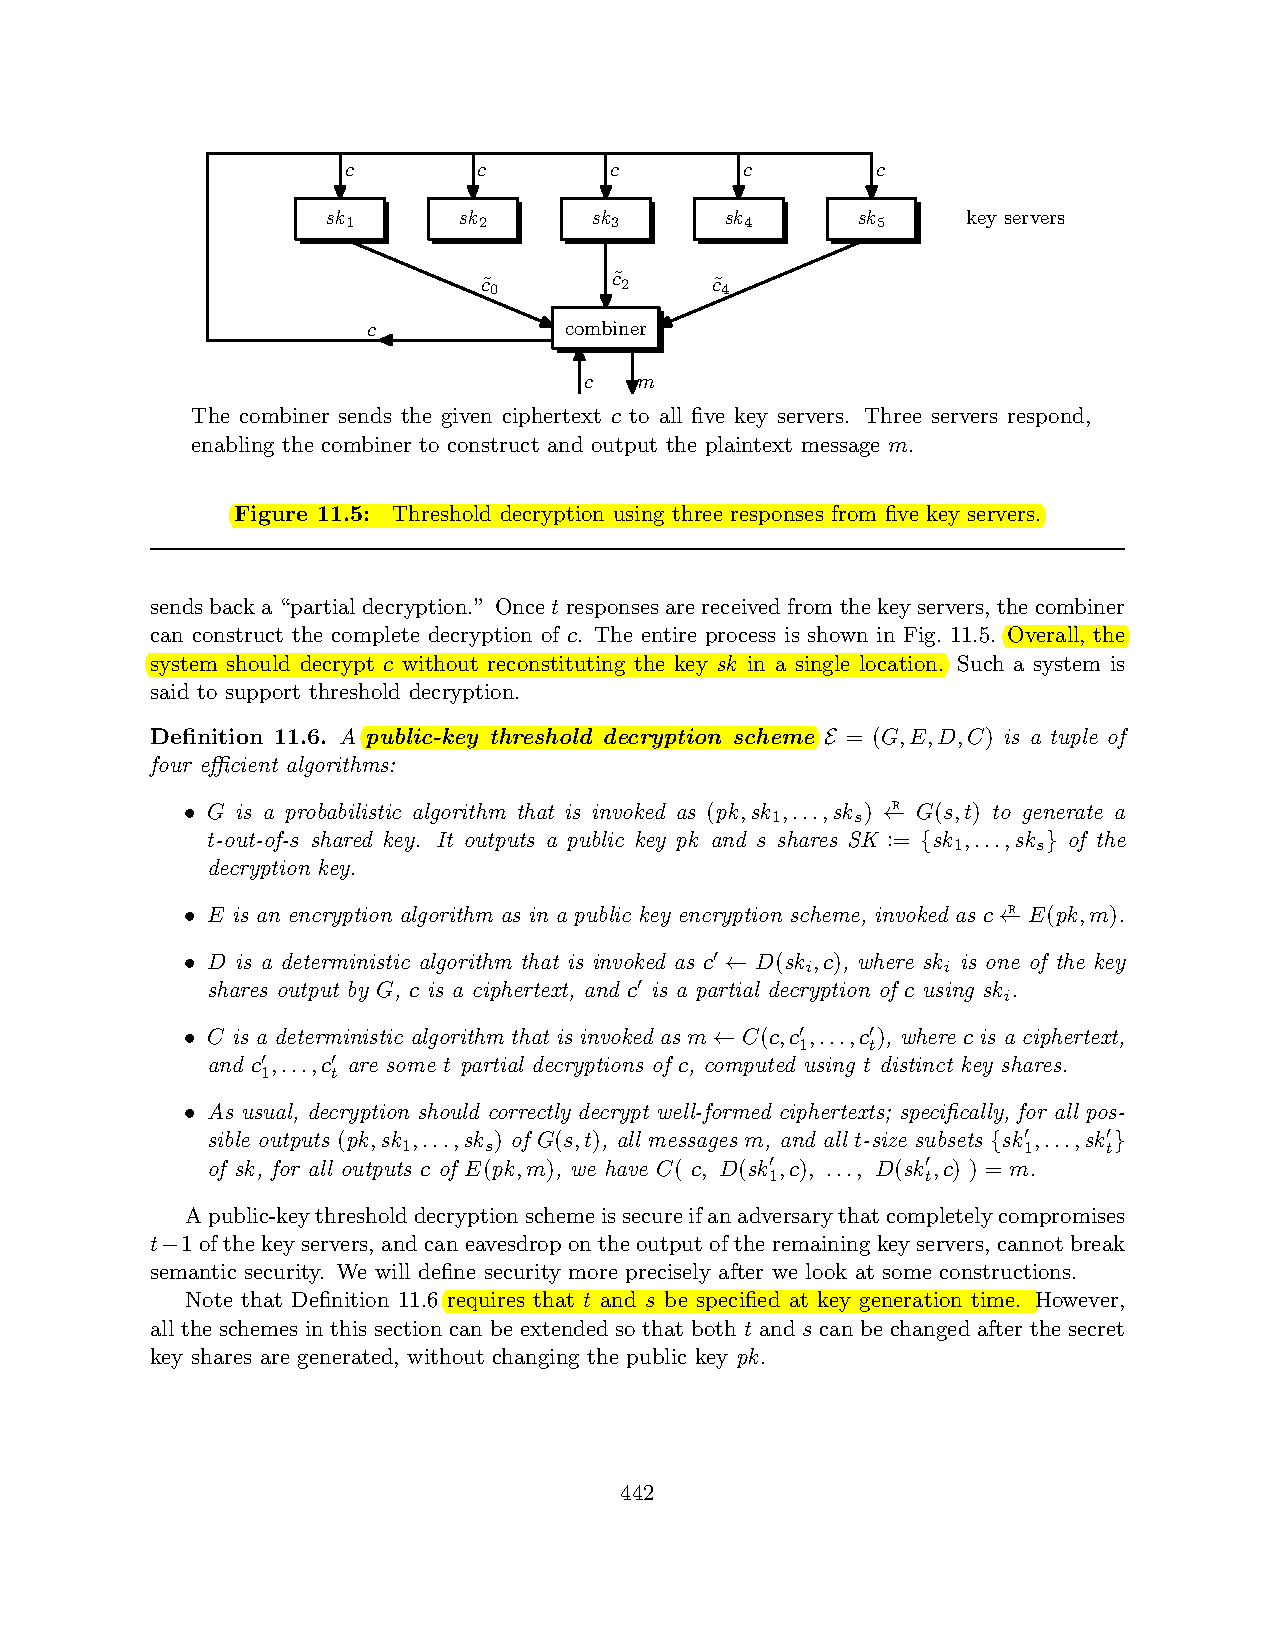
\includegraphics[clip, trim=3cm 21.2cm 3cm 2cm, width=1.00\textwidth]{img/threshold_decryption_excerpt.pdf}
    \caption{Übersicht über den Entschlüsselungsvorgang bei der Nutzung eines (3,5)-Schwellwertschemas. Entnommen aus \cite{boneh2016}.}
    \label{fig:threshold_decryption_combiner}
\end{figure}

In \cite{boneh2016} werden diese Systeme formalisiert. Ein \textit{Threshold-Public-Key-Decryption}-Schema \(\epsilon = (G, E, D, C)\) besteht aus vier Algorithmen: 

\begin{itemize}
  \item \(G(t, n, r)\) ist der Algorithmus zur Generation des öffentlichen Schlüssels \(pk\) und der \(n\) \textit{Shares} des geheimen Schlüssels \(\{sk_1, \dots, sk_n\}\). \(t\) steht für die Anzahl der zur Entschlüsselung benötigten \textit{Shares}. \(r\) ist als stellvertretend für die einfließenden Zufallswerte zu betrachten.
  
  \item \(E(pk, m, r)\) steht für den Algorithmus, der der Verschlüsselung eines Klartexts \(m\) mit dem öffentlichen Schlüssel \(pk\) dient. \(r\) dient der Vermeidung von \textit{Known-Ciphertext-Angriffen}. \todo{Vmtl.? Mehr Details...}
  
  \item \(D(sk_i, c)\) ist der Algorithmus der für einen bestimmten \textit{Share} und einen Schlüsseltext \(c\) eine partielle Entschlüsselung \(c_j'\) liefert.\todo{EZ: c' ist ungeeignet fuer die Benennung eines Entschluesselungsergebnisses, wenn du den Schluesseltext mit c bezeichnest. Wo kommt das j her?}
  
  \item \(C(c, c_1', \dots, c_t')\) ist der Algorithmus, der aus dem Schlüsseltext \(c\) und aus \(t\) durch \(D\) generierten partiellen Entschlüsselungen wieder den Klartext \(m\) liefert. Dieser Algorithmus wird auch \textit{Combiner} genannt. 
\end{itemize}

Zusätzlich wird von diesen Algorithmen die folgende Eigenschaft verlangt. Sie beschreibt die korrekte Entschlüsselung von validen Schlüsseltexten im Kontext eines Schwellwertschemas: Für alle möglichen Ergebnisse \((pk, \{sk_1, \dots, sk_n\})\) von \(G\), alle möglichen Nachrichten \(m\) und alle \(t\)-elementigen Teilmengen der \textit{Shares} \(\{sk_1', \dots, sk_t'\}\) soll für alle möglichen Schlüsseltexte \(c=E(pk, m, r)\) gelten: \(C(c, D(sk_1', c), \dots, D(sk_t', c)) = m\).

Eine Übersicht über den Entschlüsselungsvorgang ist in Abbildung \ref{fig:threshold_decryption_combiner} zu finden. Dort sind die partiellen Entschlüsselungen und der \textit{Combine}-Vorgang eines \((3,5)\)-Schwellwertschemas dargestellt. Der Algorithmus \(D\) für die partielle Entschlüsselung läuft dabei auf den einzelnen \textit{Key-Servern} ab.

In \cite{boneh2006} werden diese Algorithmen noch um einen fünften erweitert, der dazu dient, einzelne partielle Entschlüsselungen auf Validität zu überprüfen. Hierdurch können fehlerhaft handelnde \textit{Key-Server} aufgedeckt werden. Hierzu wird auch der Algorithmus \(G\) verändert, der zusätzlich einen Validierungsschlüssel \(vk\) liefert:
\begin{enumerate}
	\item \(G(t, n, r)\) liefert nun \((pk, vk, \{sk_1, \dots, sk_n\})\).
  \item[...] 
  \setcounter{enumi}{4}
	\item \(V(pk, vk, c, c_j')\) überprüft die \(j\)-te partielle Entschlüsselungen auf Validität.
\end{enumerate}

Weiterhin wird für den neuen Algorithmus eine weitere Eigenschaft verlangt. Für jeden Schlüsseltext \(c\) und \(c_j' = D(sk_i,c)\), wobei \(sk_i\) der \(i\)-te von \(G\) erstellte \textit{Share} ist, gelte: \(V(pk, vk, c, c_j')\) liefert ein valides Ergebnis.



\section{Weitere kryptographische Verfahren und Techniken}

In diesem Abschnitt werden die Grundlagen weiterer kryptographischer Verfahren und Techniken vorgestellt, die in dieser Arbeit verwendet werden.

% Aus der BA

\subsection{Hashfunktion}

Eine Hashfunktion ist eine Funktion, die eine Eingabe variabler Länge auf eine Ausgabe fester Länge (den Hashwert) abbildet.\\
In der Kryptographie werden meist kryptographisch sichere Hashfunktionen eingesetzt. Bei dieser Art von Hashfunktionen handelt es sich um Einwegfunktionen, d.h. es ist leicht, aus einer Eingabe den Hashwert zu berechnen, jedoch nicht mit vertretbarem Aufwand möglich, zu einem gegebenen Hashwert eine Eingabe zu finden, die auf diesen Wert abgebildet wird. Zusätzlich müssen die Hashfunktionen kollisionsresistent sein: Für einen gegebenen Wert ist es praktisch nicht möglich einen zweiten Wert zu finden, der den gleichen Hashwert besitzt \cite{Schneier2006}.

\subsection{Message Authentication Code}

\label{sec_mac}

Ein Message Authentication Code (MAC) ist ein Verfahren, das dazu dient, die Authentizität und die Integrität einer Nachricht sicherzustellen. Dazu wird vom Sender aus einem geheimen Schlüssel \(k\) und der Nachricht \(m\) eine Art Prüfsumme generiert und zusammen mit der Nachricht versendet. Ein Empfänger kann den MAC überprüfen, wenn er im Besitz des gleichen geheimen Schlüssels ist, und so sicher sein, dass die Nachricht nicht verändert wurde \cite{Schneier2006}.

\subsection{Hybride Kryptosysteme}

\label{sec_basics_hybrid}

Als hybrides Kryptosystem wird die Kombination von symmetrischen und asymmetrischen Kryptoverfahren zur Verschlüsselung bzw. Entschlüsselung einer Nachricht bezeichnet. Ein Schlüssel \(k_{symm}\) für die Verwendung im symmetrischen Verfahren wird zufällig erzeugt und mithilfe des öffentlichen Schlüssels eines asymmetrischen Verfahren als \(c_{public}\) verschlüsselt. Der zu verschlüsselnde Klartext \(m\) wird anschließend mithilfe des symmetrischen Verfahrens und des erzeugten Schlüssels \(k_{symm}\) als Chiffretext \(c_{symm}\) verschlüsselt. \\
Zur Entschlüsselung wird \(c_{public}\) mit dem geheimen Schlüssel des asymmetrischen Verfahrens entschlüsselt. Der hieraus erhaltene Schlüssel \(k_symm\) kann nun zur Entschlüsselung von \(c_{symm}\) genutzt werden, um \(m\) zu erhalten \cite{katz2014}.

Der Vorteil dieser Lösung beruht darin, dass Vorteile symmetrischer und asymmetrischer Verfahren kombiniert werden: Symmetrische Verfahren sind im Allgemeinen deutlich schneller als asymmetrische, die jedoch das bei symmetrischen Systemen bestehende Problem des Schlüsselaustauschs lösen.

\subsection{Authenticated Encryption Schemes}

\label{sec_basics_ae}

Symmetrische Kryptosysteme sorgen erst einmal nur für den Schutz der Vertraulichkeit einer Nachricht. Wird zusätzlich die Integrität einer Nachricht durch das System geschützt, so spricht man von einem \textit{Authenticated Encryption Scheme}. Hierdurch wird erreicht, dass Änderungen am Schlüsseltext bei der Entschlüsselung erkannt werden und der Vorgang abgebrochen werden kann.\\
Ein solches System kann durch Berechnung eines MACs zusätzlich zur Verschlüsselung erreicht werden. Alternativ dazu gibt es Schemata, die direkt auf einer Blockchiffre aufbauen \cite{boneh2016}. Ein Beispiel hierzu ist der GCM-Betriebsmodus, der in Kombination mit AES in vielen verbreiteten Protokollen wie TLS zu finden ist.


\subsection{ElGamal-Kryptosystem}

\label{sec_basics_threshold_elgamal}

Im Folgenden sei \(\mathbb{G}\) eine zyklische Gruppe der primen Ordnung \(p\) und \(g\) ein Generator dieser Gruppe. Diese Parameter können öffentlich bekannt gegeben werden. Alle folgenden Berechnungen werden in \(\mathbb{G}\) (also modulo \(p\)) ausgeführt.

Ein Teilnehmer wählt nun ein zufälliges Element \(x \in \mathbb{Z}_p\). Dies ist der private Schlüssel des Teilnehmers. Er berechnet zusätzlich seinen öffentlichen Schlüssel \(h = g^x\).\\
Um eine Nachricht \(m\), die an den Teilnehmer geschickt werden soll, zu verschlüsseln, wird zuerst ein zufälliges Element \(y \in \mathbb{Z}_p\) gewählt. Anschließend kann die Nachricht verschlüsselt als \((v, c) = (g^y, h^y \cdot m)\) versendet werden.\\
Zur Entschlüsselung berechnet der Empfänger \(k' = (v^x)^{(-1)}\) und kann die Nachricht \(m = c \cdot k'\) entschlüsseln. Dies funktioniert, da 
\[c \cdot k' = (h^y \cdot m) \cdot (v^x)^{(-1)} = g^{xy} \cdot m \cdot g^{(-yx)} = m\]
gilt.

Die Sicherheit des Verfahrens beruht auf dem Diskreten-Logarithmus-Problem. Details und Beweise hierzu sind beispielsweise in \cite{katz2014} zu finden. \todo{Erweitern, um später darauf zurückgreifen zu können}


\section{Searchable Symmetric Encryption}

\label{sec_basisc_se}

%- Searchable Symmetric encryption vs Public Key Encryption With Keyword Search
%- Hier relevant SSE

\textit{Searchable Symmetric Encryption} (SSE) ist ein Konzept , das es ermöglicht, Daten in verschlüsselter Form auf einen Server auszulagern und trotzdem Suchanfragen auf den Daten ausführen zu können. Ein allgemeines SSE-Schema besteht aus vier effizient berechenbaren Algorithmen \cite{wang2016}:

\begin{itemize}
  \item \textbf{GenerateKey}\((k)\) generiert einen geheimen Schlüssel \(K\) anhand eines (verfahrensabhängigen) Sicherheitsparameters \(k\).
  \item \textbf{BuildIndex}\((K, D)\) erstellt einen Suchwort-Index \(I\) aus dem generierten Schlüssel \(K\) und einer Dokumentenmenge \(D\).
  \item \textbf{GenerateTrapdoor}\((K, w)\) erstellt für ein spezielles Suchwort \(w\) mithilfe des Schlüssels \(K\) das Trapdoor-Element \(T_w\) für die Suche nach \(w\).
  \item \textbf{Search}\((I, T_w)\) liefert eine Menge von Dokumenten basierend auf einem Suchwort-Index \(I\) und einem Trapdoor-Element \(T_w\).
\end{itemize}

Der Besitzer der Daten erstellt sich einen Schlüssel mithilfe von \textbf{GenerateKey} und generiert durch \textbf{BuildIndex} einen Suchwort-Index für seine Dokumente. Anschließend lädt er diese Dokumente in verschlüsselter Form zusammen mit dem Index auf den Server. Möchte der Besitzer nun alle Dokumente erhalten, auf die ein spezielles Suchwort zutrifft, so erstellt er für dieses Suchwort mithilfe von \textbf{GenerateTrapdoor} ein Trapdoor-Element und sendet dieses an den Server. Dort wird nun auf dem Suchwort-Index durch \textbf{Search} die Suche nach dem Trapdoor-Element ausgeführt, die eine Menge von verschlüsselten Dokumenten liefert, auf die das Suchwort zutrifft. Diese können zurück an den Besitzer gesendet werden, der sie lokal entschlüsseln kann. 

\chapter{Ueberblick}

\todo{Einführendes mit High-Level-Übersicht}


Dazu werden in diesem Kapitel zentrale Anforderungen an ein solches System entwickelt und eine abstrakte Architektur entworfen. Begonnen wird jedoch mit der Erstellung eines Angreifermodells, das eine zentrale Voraussetzung für die nachfolgenden Schritte darstellt.

\section{Zugrundeliegendes Angreifermodell}

\label{subsec_impl_requirements_attackermodel}

% Das Angreifermodell definiert die	maximal	berücksichtigte	Stärke eines Angreifers, gegen den ein	Schutzmechanismus	gerade noch wirkt.	
%Es beschreibt:
%–  Rollen des Angreifers (Außenstehender, Benutzer, Betreiber, Wartungsdienst, Produzent, Entwerfer …), auch kombiniert 
%–  Verbreitung des Angreifers (Stellen im System, an denen der Angreifer Informationen gewinnen oder Systemzustände verändern kann) 
%–  Verhalten des Angreifers 
%  •  passiv / aktiv,  beobachtend / verändernd 
%–  Rechenkapazität des Angreifers 
%  •  unbeschränkt: informationstheoretisch 
%  •  beschränkt: komplexitätstheoretisch 

Im Kontext dieser Arbeit, die sich mit der datenschutzfreundlichen Speicherung von Überwachungsdaten beschäftigt, muss zuerst folgende Vorüberlegung getroffen werden: Logdaten erreichen das verwendete SIEM-System abhängig von den verwendeten Protokollen im allgemeinen nicht-pseudonymisiert und oftmals weder verschlüsselt noch mit geschützer Integrität über das Netzwerk. \todo{Angriffsmöglichkeiten erläutern: Mitschneiden aller Daten und damit  Aufdecken von Pseudonymen, ...}
Diese Angriffsmöglichkeiten zu verhindern, ist ausdrücklich kein Ziel dieser Arbeit. Daher bezieht sich das Angreifermodell auf die Bearbeitung und Speicherung von Logdaten, erst sobald sie das zu entwickelnde System erreichen, jedoch nicht vorher.

Das Ziel des Systems bezogen auf seine Sicherheit lässt sich folgendermaßen definieren: Das Pseudonym eines Nutzers erlaubt (ohne Anwendung von Hintergrundwissen) keinen Rückschluss auf die Identität eines Nutzers. Erst die Kollaboration berechtigter Akteure ermöglicht das Aufdecken eines Pseudonyms.\todo{? außerdem erweitern um aktive Angreifer?}

Ein Angreifermodell beschreibt die maximale Stärke eines Angreifers im Bezug auf verschiedene Faktoren, gegen die ein System abgesichert ist. Enthalten sind die Rolle eines Angreifers, seine Verbreitung im System, aktives oder passives Verhalten und die Rechenkapazität, die der Angreifer zum Überwinden der eingesetzten Schutzmaßnahmen aufbringen kann. Es bildet die Basis für alle Folgeüberlegungen im Bezug auf die Sicherheit des zu entwickelnden Systems.

Für das Angreifermodell werden folgende Annahmen getroffen: Bei dem Angreifer kann es sich um einen Außenstehenden, um einen Berechtigten mit Zugriff auf das SIEM-System oder sogar um einen Administrator mit physischem Zugriff auf Rechner im Netz handeln. Wie bereits beschrieben, wird die ungesicherte Übertragung nicht-pseudonymisierter Daten zu dem System nicht betrachtet. Insofern wird von einem Angreifer ausgegangen, der erst Zugriff auf das zu entwickelnde System oder das SIEM-System beseitzt oder erlangt. Das zu entwickelnde System soll in der Lage sein, sich auch gegen aktive Angreifer zur Wehr zu setzen. \todo{Denial of Service etc?}
Bezogen auf die verfügbare Rechenleistung des Angreifers sollen verbreitete und nach heutigem Wissensstand für sicher befundene kryptographische Algorithmen als nicht mit vertretbarem Aufwand zu brechen angesehen werden. Es handelt sich daher um die Annahme von komplexitätstheoretischer Sicherheit.


\section{Anforderungen}

\label{sec_impl_requirements}

Neben den primären Anforderungen, die sich direkt aus der Funktionsbeschreibung des Systems und dem Zusammenspiel der enthaltenen Verfahren ergeben, sollte das System noch weitere Eigenschaften wie beispielsweise die Erweiterbarkeit um zusätzliche Datenschutztechniken erfüllen. All diese Anforderungen sollen im folgenden Abschnitt aufgestellt und näher erläutert werden.

\subsection{Integration in das SIEM-System}

\label{subsec_impl_requirements_ossimintegration}

Für den Eingriff in den Datenfluss der Logdaten zwischen ihrer Quelle und dem verwendeten SIEM-System muss eine geeignete Stelle gefunden werden. Hierzu müssen Auswirkungen des Eingriffs betrachtet sowie die Vor- bzw. Nachteile der verschiedenen Möglichkeiten gegeneinander abgewogen werden. 

\subsection{Pseudonymisierung}

\label{subsec_impl_requirements_pseudonymity}

%- Lang genug für geringe Kollisionswsk.
%- Eindeutig
%- Durchsuchbar (mim Hinblick auf threshold)
%- Anwendungsfallabhängige Parameter für Nutzzeit, ... (Rückblick auf Kapitel 3)

Die Pseudonymisierung muss es ermöglichen, nach Aufdecken eines Eintrags wieder auf den ursprünglichen Dateninhalt schließen zu können. Daher müssen die Pseudonyme für die Zeit ihrer Speicherung eindeutig sein, d.h. es darf zu keiner Mehrfachverwendung von Pseudonymen kommen. 

Weiterhin muss es beim Pseudonymisieren von Logeinträgen eine Möglichkeit geben, zu überprüfen, ob für ein Datum bereits ein Pseudonym vergeben wurde. So kann sichergestellt werden, dass in einem bestimmten Zeitraum Logeinträge zu einer Person stets mit dem gleichen Pseudonym versehen werden, um mithilfe der Verknüpfung von Einträgen Anomalieerkennungsverfahren sinnvoll einsetzen zu können. Auf diese Anforderung wird in Abschnitt \ref{sec_state_se} noch genauer eingegangen.

Außerdem muss es eine Möglichkeit geben, die Parameter der Pseudonymisierung, wie den Zeitraum ihrer Verwendung, konfigurierbar zu machen (siehe Abschnitt \ref{sec_state_pseudonymity}).

\subsection{Einsatz eines kryptographischen Schwellwertschemas}

\label{subsec_impl_requirements_threshold}

%- Verteiltes Modell 
%- Kommunikation
%- Schlüsselmanagement
%- ...

Der Einsatz eines kryptographischen Schwellwertschemas setzt eine verteilte Anwendung voraus, die den Zugriff für die Pseudonymisierungskomponente sowie für die bei der Entschlüsselung eines Eintrags beteiligten Akteure bereitstellt. Die für das Schwellwertschema nötigen, in Abschnitt \ref{sec_basics_threshold} beschriebenen Parameter \(t\) und \(n\) und auch die beteiligten Share-Besitzer müssen in dem System initial konfigurierbar sein.

In der Phase der Schlüsselgenerierung muss das System die Kommunikation und Koordination aller Beteiligten unterstützen. Die hier erstellten Schlüssel und \textit{Shares} müssen an geeigneten Stellen sicher gespeichert und abrufbar sein. Für diese Phase gibt es zwei Möglichkeiten:
\begin{itemize}
  \item \textbf{Zentrale Generierung von öffentlichem Schlüssel und Shares}: Eine vertrauenswürdige Komponente generiert ein Schlüsselpaar und zerlegt den geheimen Schlüssel in die einzelnen Shares, die anschließend verteilt werden können. 
  \item \textbf{Verteilte Schlüsselgenerierung}: Hierbei generieren die einzelnen Share-Besitzer jeweils ihre eigenen Shares. Durch verteilte Berechnungen kann hieraus der gemeinsame öffentliche Schlüssel erzeugt werden. Der geheime Schlüssel liegt auf diese Weise niemals an einer Stelle vor und ein vertrauenswürdiger Dritter ist nicht notwendig. Aus diesem Grund ist diese Lösung zu bevorzugen.
\end{itemize}

Der für die Verschlüsselung erforderliche öffentliche Schlüssel muss so vorliegen, dass er bei der Verschlüsselung eines Pseudonym-Datensatzes genutzt werden kann.

Bei der Entschlüsselung eines Eintrags, also der Aufdeckung eines Pseudonyms, muss das System wiederum die beteiligten Akteure koordinieren. Anschließend muss eine Komponente die Rolle des \textit{Combiners} übernehmen, so dass anschließend der den Pseudonymhalter beschreibende, entschlüsselte Datensatz im System  vorliegt.

\subsection{Benutzerinteraktion}

\label{subsec_impl_requirements_userinteraction}

%- Proxy: Konfiguration der Plugins

%- Pseudo-App: Statusanzeige angemeldeter Benutzer(Admin), Initialisierung der Schlüsselgenerierung nach Nutzerauswahl(Admin), Anlegen von Aufdeckanfragen, Statusanzeige von Aufdeckanfragen, Systemstatus

%- Einzelne Teilnehmer sollten Client-Anwendungen besitzen, um auf Anfragen reagieren zu können (Generation eigener Schlüssel, gemeinsame Schlüsselgenerierung, ... ) Konsolenanwendung? 

Die zu entwickelnde verteilte Anwendung wird an verschiedenen Stellen Benutzerinteraktion erfordern.

Das Konfigurieren des Systems zur Integration verschiedener Datenquellen muss einem berechtigten Nutzer zugänglich gemacht werden. Ebenso sollte es für die -- in der Aufgabenstellung geforderte -- Erweiterbarkeit um weitere Datenschutztechniken relativ leicht sein, diese Techniken im System nutzen zu können. 

Für pseudonymisierte Datensätze muss es berechtigten Benutzern ermöglicht werden, Anfragen zur Aufdeckung eines Pseudonyms zu stellen und sich über ihren Status informiert zu halten.

Einem Administrator des Systems sollte es für die Benutzung eines kryptographischen Schwellwertschemas ermöglicht werden, grundlegende Parameter des Systems wie die Schwellwertparameter und die beteiligten Nutzer auszuwählen sowie die Initialisierung des Schemas anzustoßen. 

Die am Schwellwertschema beteiligten Nutzer müssen die Möglichkeit erhalten, eine Übersicht über sie betreffende Anfragen zur Aufdeckung eines Pseudonym-Datensatzes zu bekommen sowie einzelne Anfragen abzulehnen oder sich am Prozess des Aufdeckens mithilfe des Schwellwertschemas zu beteiligen. 

\subsection{Erweiterbarkeit um neue Datenquellen}

\label{subsec_impl_requirements_differentsources}

Das umzusetzende System sollte es ermöglichen, Daten aus verschiedenen Quellen und (abhängig vom gewählten Eingriffspunkt in OSSIM) auch in verschiedenen Formaten entgegenzunehmen und mithilfe der umgesetzten Datenschutztechniken verändern zu können. Dabei muss das Format der Logdaten grundsätzlich beibehalten werden, um die Behandlung der Daten in dem verwendeten SIEM-System weiterhin zu ermöglichen.

\subsection{Erweiterbarkeit um neue Datenschutztechniken}

\label{subsec_impl_requirements_plugins}

Neben der im Fokus dieser Arbeit stehenden Pseudonymisierung und dem Einsatz von kryptographischen Schwellwertschemata zum Schutz der Logdaten gibt es weitere Datenschutztechniken, die für den Anwendungsfall genutzt werden könnten (siehe Kapitel \ref{cha_alternatives}). Das zu entwickelnde System sollte leicht um diese Techniken erweiterbar sein, d.h. so gestaltet sein, dass andere Techniken ohne große Änderungen am System integriert und auf eingehende Logdaten angewendet werden können.

\subsection{Performanz}

Das System sollte es, eingesetzt in einem Unternehmensnetzwerk, ermöglichen eine ausreichende Menge von Logdaten in einer bestimmten Zeitspanne behandeln zu können. 

\subsection{Übersicht}

Ein System, wie es in dieser Arbeit angestrebt wird, sollte also folgende Eigenschaften aufweisen:

\begin{itemize}
  \item Geeignete Stelle zum Eingriff in den Datenfluss zwischen Logdatenquelle und SIEM-System,
  \item parameterabhängige Generierung eindeutiger, aber in gewissem Rahmen verknüpfbarer Pseudonyme,
  \item sicherer, verteilter Einsatz eines anpassbaren kryptographischen Schwellwertschemas -- vorzugsweise mit verteilter Schlüsselgenerierung,
  \item geeignete Benutzerinteraktion mit dem System an notwendigen Stellen,
  \item Erweiterbarkeit um unbekannte Datenquellen,
  \item Erweiterbarkeit um weitere Datenschutztechniken,
  \item Performanz.
\end{itemize}


\section{Entwurf}

\label{sec_impl_architecture}

In diesem Abschnitt wird basierend auf den Anforderungen aus Abschnitt \ref{sec_impl_requirements} eine von eingesetzten Verfahren unabhängige Architektur für das System entworfen. Der erste Unterabschnitt beschäftigt sich mit der Frage, an welcher Stelle in den Datenfluss zwischen Quelle der Logdaten und SIEM-System eingriffen werden kann. Anschließend wird basierend hierauf die Systemarchitektur erstellt.

\subsection{Eingriff in den Datenfluss des SIEM-Systems}

\label{sec_over_dataflow_siem}

Für den Eingriff zur Pseudonymisierung der Logdaten bieten sich verschiedene Stellen im Datenfluss eines SIEM-Systems an. Im Folgenden sollen diese Möglichkeiten dargestellt und bezogen auf die in Abschnitt \ref{subsec_impl_requirements_ossimintegration} dargestellten Eigenschaften bewertet werden:
\begin{itemize}
  \item Veränderung des SIEM-Systems
  \item Nicht-pseudonymisierte Daten im SIEM-System
  \item Mehrfaches Parsen von Logdaten
  \item Abhängigkeit von Besonderheiten des SIEM-Systems
\end{itemize}
Eine Übersicht über die verschiedenen Stellen bietet Abbildung \ref{fig:siem_data_access_point}. Die Ziffern der Möglichkeiten beziehen sich auf die in der Abbildung gekennzeichneten Stellen.

\begin{figure}[]
    \centering
        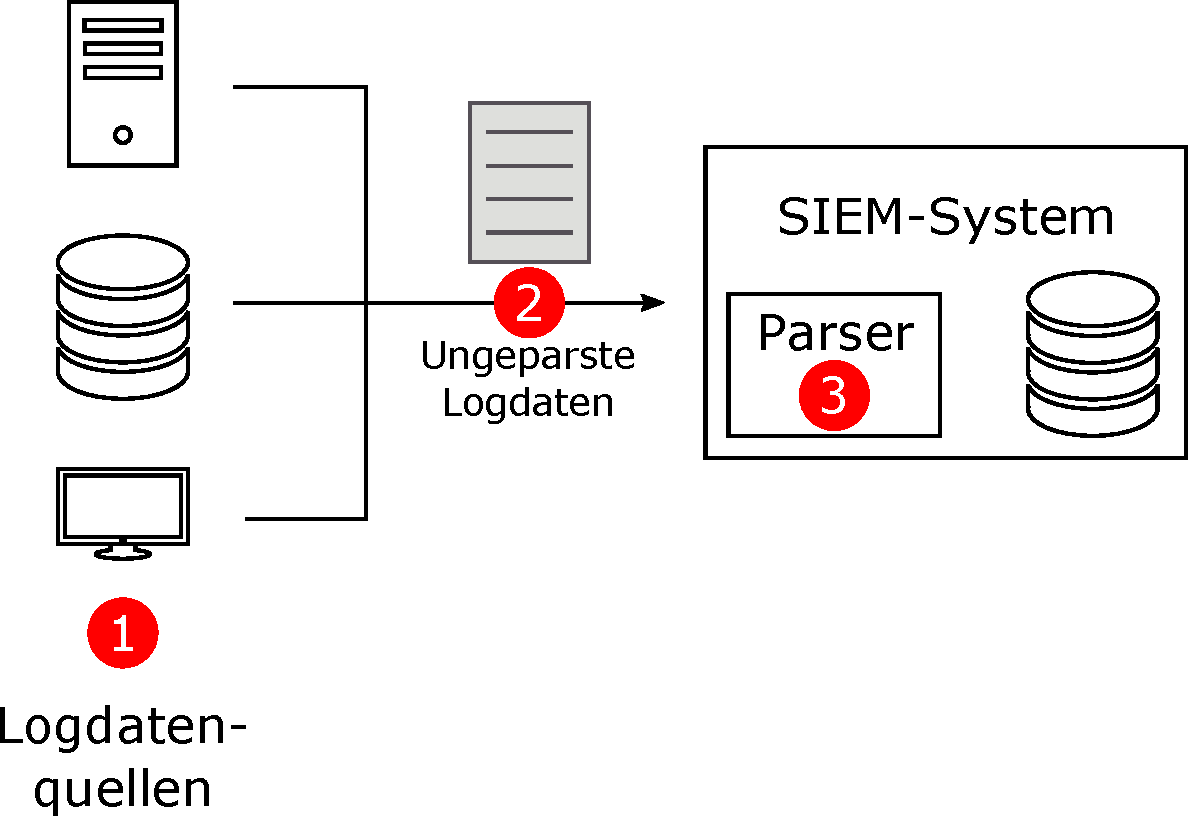
\includegraphics[width=0.5\textwidth]{dia/siem_data_access_point.pdf}
    \caption{Mögliche Eingriffspunkte in den Datenfluss eines SIEM-Systems.}
    \label{fig:siem_data_access_point}
\end{figure}

\begin{enumerate}

\item \textbf{In der Quelle der Logdaten}\\
  Bei diesem Ansatz werden die Daten bereits pseudonymisiert, bevor sie die Datenquelle verlassen. Dieser Ansatz sorgt dafür, dass die Daten bereits pseudonymisiert auf der Übertragungsstrecke und im SIEM-System vorliegen. Es ist kein mehrfaches Parsen der Daten notwendig und der Ansatz ist unabhängig vom verwendeten SIEM-System zu realisieren. Auf der anderen Seite macht der Ansatz die universelle Veränderung jeder Datenquelle notwendig. Dies kann bei Datenquellen, die auf ähnlichen gut erweiterbaren Plattformen beruhen, relativ einfach umzusetzen sein. Beispielsweise könnte die im nächsten Ansatz vorgestellte Proxy-Komponente lokal auf der Datenquelle eingesetzt werden. Schwierigkeiten würde dieser Ansatz hingegen bei Datenquellen bereithalten, die beispielsweise aus Gründen abgespeckter zugrundeliegender Betriebssysteme oder geringer Rechenleistung nur schwer erweiterbar sind. Außerdem würde er in vielen Fällen die Kooperation des Herstellers voraussetzen, wenn es sich um nicht quelloffene \glqq{}Box\grqq{}-Lösungen handelt.

\item \textbf{Proxy-basierter Ansatz}\\
  Dieser Ansatz pseudonymisiert die Daten vor dem ersten Kontakt mit dem SIEM-System, indem Datenquellen ihre Logdaten an einen Proxy senden, der die Daten pseudonymisiert und erst anschließend an das SIEM-System weiterreicht. Hierdurch wird erreicht, dass die Daten zu keiner Zeit nicht-pseudonymisiert in dem SIEM-System vorliegen. Außerdem ist er unabhängig von Datenquellen und SIEM-System und erfordert keinen direkten Eingriff in diese (abgesehen von geringen Konfigurationsanpassungen). Ein Nachteil dieser Lösung ist, dass sie das Parsen und Neuzusammensetzen der Logdaten im Proxy zusätzlich zu deren anschließender Behandlung im SIEM-System erfordert. Außerdem müssen für verschiedene Arten der Logdatenübermittlung (Protokolle wie syslog oder SNMP) unterschiedliche Proxys entwickelt werden.

\item \textbf{Patchen des SIEM-Systems}\\
  Die letzte Möglichkeit ist das Verändern des SIEM-Systems selbst. Hierzu wird in die Logdaten parsende Komponente eingegriffen, um vor, während oder nach diesem Vorgang die Logdaten zu pseudonymisieren. Dieser Ansatz erfordert kein mehrfaches Bearbeiten von Logdaten wie in dem Proxy-basierten Ansatz. Auf der anderen Seite ist er abhängig vom eingesetzten SIEM-System und erfordert seine Veränderung. Zusätzlich liegen die Daten erst einmal in nicht veränderter Form im SIEM-System vor, was die in Abschnitt \ref{subsec_impl_requirements_ossimintegration} erwähnten Nachteile mit sich bringt.

\end{enumerate}

Aus datenschutztechnischer Sicht ist eine frühestmögliche Pseudonymisierung zu bevorzugen, wie sie auch in \cite{schwartmann2017} empfohlen wird: 
\glqq{}Die Pseudonymisierung ist im Verarbeitungsprozess so früh wie möglich durchzuführen.\grqq{}
Daher wäre eine Pseudonymisierung bereits in der Datenquelle der Optimalfall. Demgegenüber stehen jedoch die erwähnten Nachteile des ersten Ansatzes im Bezug auf die Umsetzbarkeit, da hierzu jede mögliche Quelle von Logdaten universell verändert werden müsste. Eine erst im SIEM-System stattfindende Pseudonymisierung bringt jedoch die beschriebenen Risiken im Bezug auf das Vorliegen des pseudonymisierten Daten im Originalformat mit.

Dies ließ die Entscheidung auf den Proxy-basierten Ansatz fallen. Dass die Lösung außerdem noch keine Anpassungen an dem SIEM-System selbst erfordert, wiegt den Nachteil des zusätzlichen Parsens und wieder Zusammensetzens der Lognachricht bei Weitem auf.
\todo{Auch auf Angreifermodell beziehen?}

\subsection{Architektur}

%- Wie deckt dieser Ansatz die Anforderungen ab?
%  - Einbindung OSSIM
%  - Pseudonymisierung
%  - Schwellwert
%  - Benutzerinteraktion
%  - Erweiterbarkeit Datenquellen
%  - Erweiterbarkeit Datenschutztechniken

Ausgehend von diesen Überlegungen wurde ein System entworfen, dass die Anforderungen aus Abschnitt \ref{sec_impl_requirements} erfüllt und an der beschriebenen Stelle in den Datenfluss eingreift. 

%\todo{Hier erweitern: Warum verteilte Lsg (ProxyPlugin - Service):
%  - Erweiterbarkeit (Mehrere Proxy-Server mit verschiedenen Protokollen, evtl. auch direkt Client-seitig, ...) => Absicherung einer Komponente, die jedoch auch nicht alles erfährt
%  - Trennung Verarbeitung und Speicherung (Kompr. DB -> Pseudonyme bleiben verdeckt, Kompr. Proxy -> bisherige Daten und Daten evtl. anderer Proxys bleiben abgesichert)
%}

Bei dem Entwurf handelt es sich um ein verteiltes System, bei der die Verarbeitung der Logdaten und die Speicherung der Pseudonymzuordnung an unterschiedlichen Stellen geschieht. Hierfür sprechen verschiedene Gründe. Die Kompromittierung der speichernden Komponente schützt die erstellten Pseudonyme vor Aufdeckung durch die Verschlüsselung der Datensätze mit einem kryptographischen Schwellwertschema. Die Kompromittierung der verarbeitenden Komponente lässt zwar eine Verknüpfung neu erstellter Pseudonyme mit eintreffenden Daten zu, sorgt aber nicht für eine Aufdeckung bereits erstellter Pseudonyme, da diese in der anderen Komponente vorliegen. Weiterhin sorgt dieser Ansatz auch für eine zusätzliche Erweiterbarkeit des Systems. Eine speichernde Komponente kann so als Datenspeicher für mehrere verarbeitende Komponenten agieren, was beispielsweise die Erweiterung um zusätzliche Protokolle (vgl. Abschnitt \ref{sec_impl_integration_into_ossim}) oder Pseudonyme über verschiedene Datenarten (vgl. Abschnitt \ref{sec_state_se_furtherpossibilities}) ermöglicht.
Einen Überblick über den Entwurf bietet Abbildung \ref{fig:high__level_architecture}. Die verschiedenen Komponenten des Systems werden im Folgenden näher beschrieben.

\begin{figure}[]
    \centering
        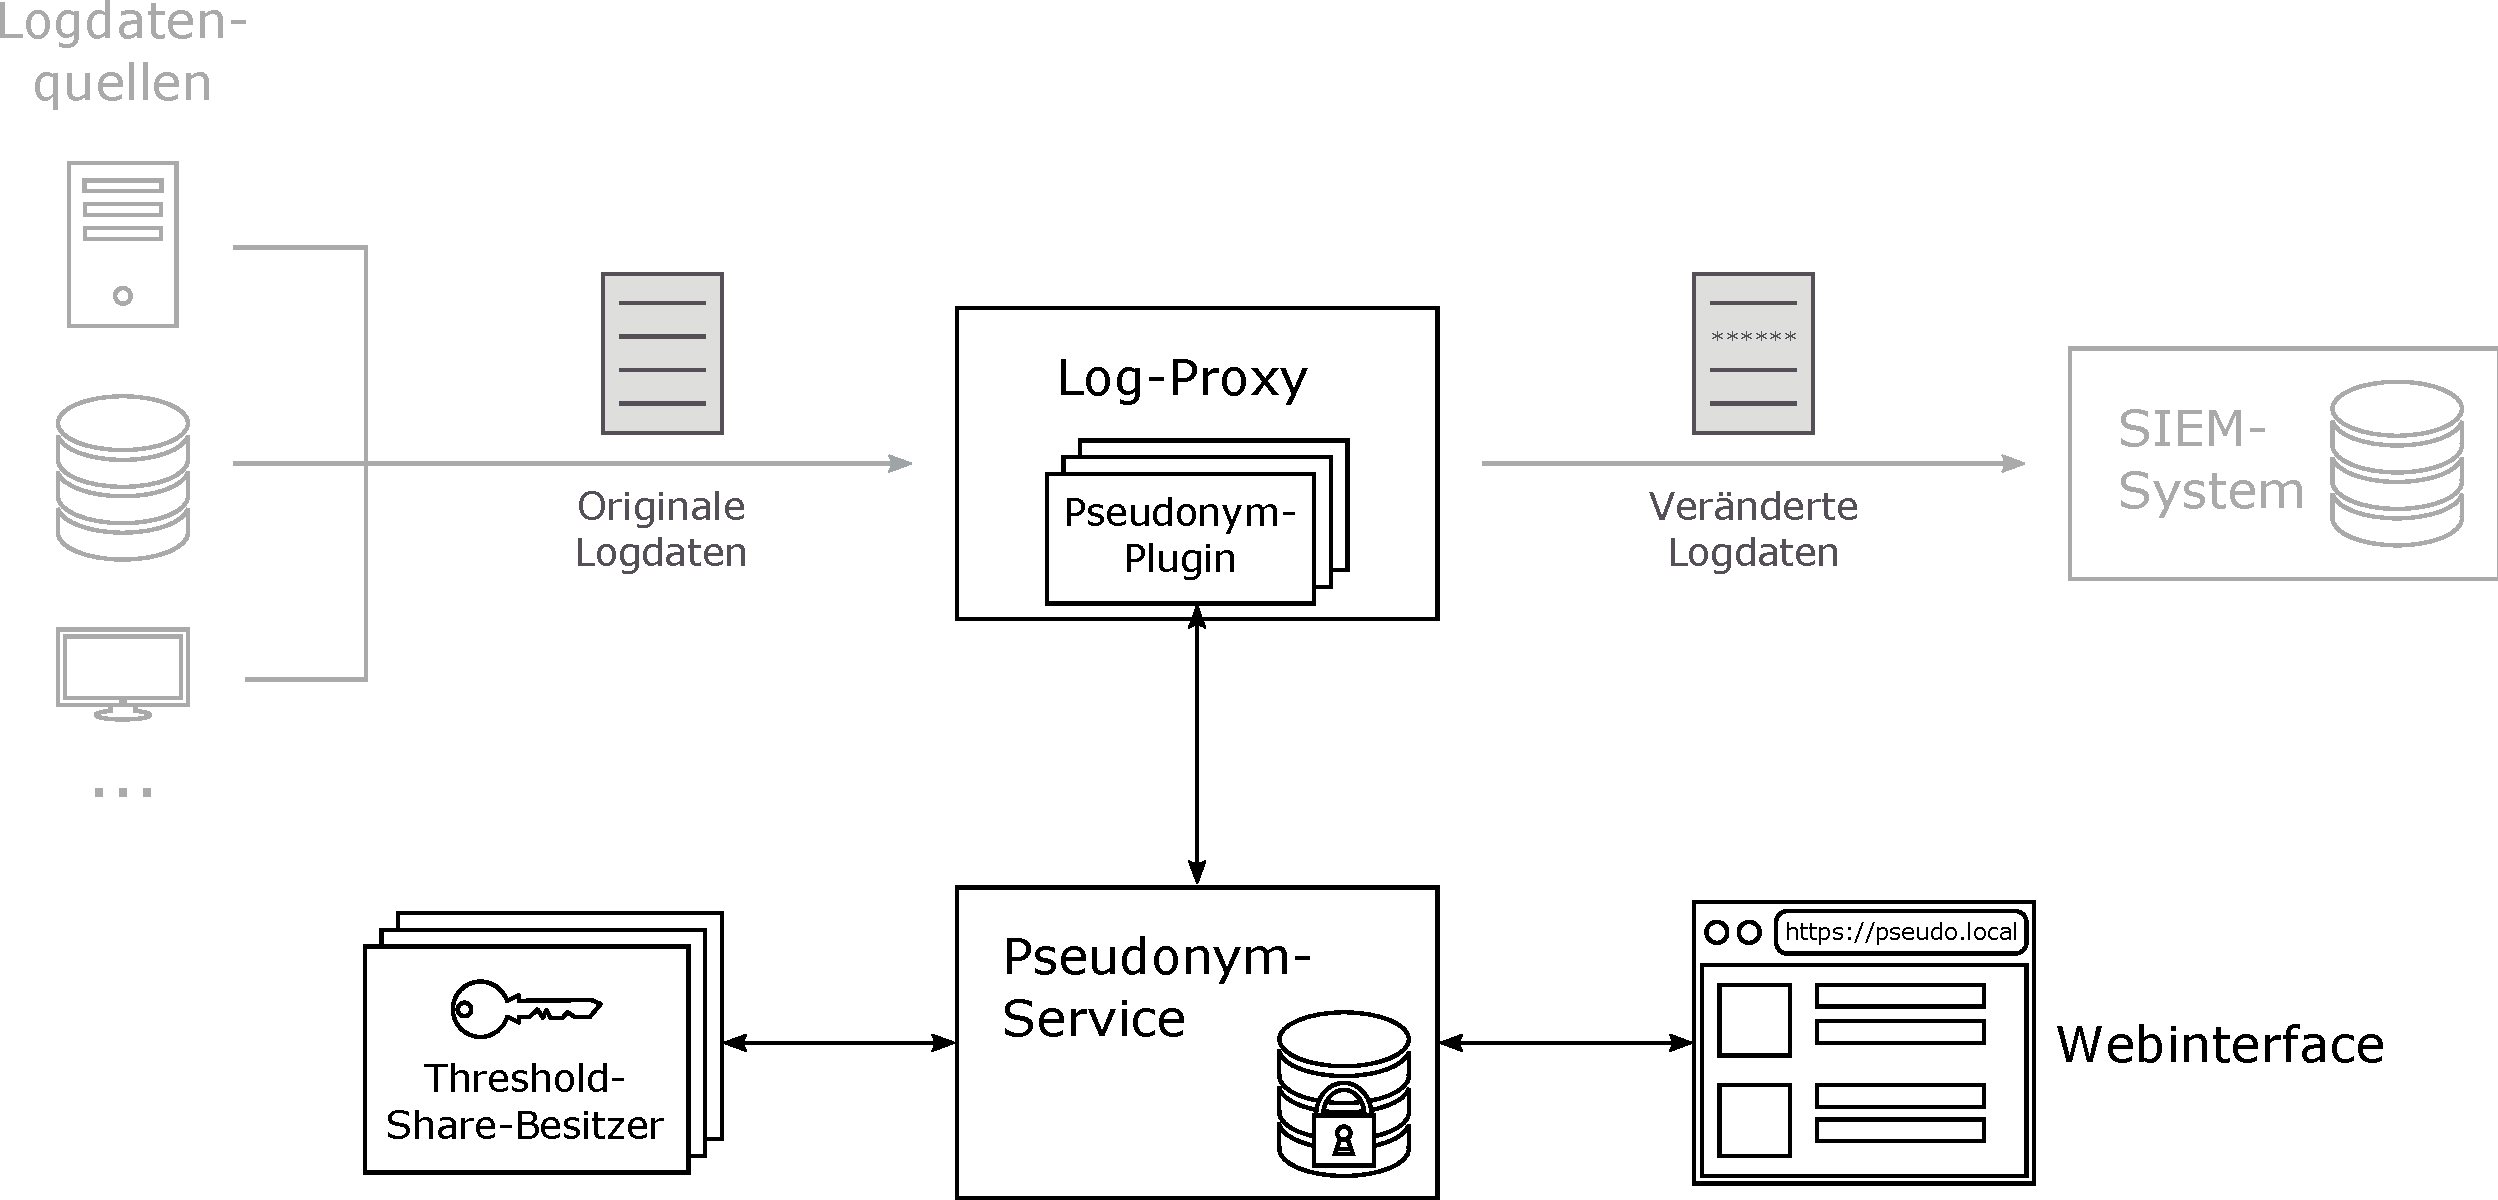
\includegraphics[width=0.9\textwidth]{dia/high_level_architecture.pdf}
    \caption{Ein Überblick über die entworfene Architektur.}
    \label{fig:high__level_architecture}
\end{figure}

Die erste Komponente ist der \textbf{Log-Proxy}, der die Daten entgegennimmt, verändert und anschließend an das SIEM-System weiterleitet. Das Verändern der Daten kann mit verschiedenen Plugins geschehen, so dass neben der umzusetzenden Pseudonymisierung auch weitere Datenschutztechniken eingesetzt werden können, was die geforderte Erweiterbarkeit aus Abschnitt \ref{subsec_impl_requirements_plugins} ermöglicht. Der Proxy leistet die Behandlung von Logdaten aus verschiedenen Quellen wie in Abschnitt \ref{subsec_impl_requirements_differentsources} beschrieben. Das für diese Art des Dateneingriffs erforderliche Parsen und Wiederzusammensetzen der Daten muss hier Datenquellen-abhängig konfigurierbar geschehen.

Ein in dem Proxy enhaltenes Plugin ist für die Pseudonymisierung von Daten zuständig und kommuniziert dazu mit einer externen Komponente -- dem Pseudonym-Service. Die Kommunikation mit dem Proxy erfolgt über einen Webservice-basierten Ansatz. Das Plugin kann für eingehende Daten ein Pseudonym anfordern und dieses anschließend in der Logdatenverarbeitung verwenden.

Der \textbf{Pseudonym-Service} erfüllt zwei Aufgaben: das Speichern und Verwalten der Pseudonyme sowie die Integrierung des kryptographischen Schwellwertschemas. Initial muss die Schlüsselgenerierung des Schwellwertschemas durch den Service geleistet werden. Dies kann wie bereits im vorhergehenden Abschnitt beschrieben zentral oder verteilt geschehen.\\
Es können während des Betriebs neue Pseudonyme angelegt und zusammen mit ihrem durch das Schwellwertschema verschlüsselten Datum abgelegt werden. Sie werden durch geeignete Maßnahmen durchsuchbar gehalten, um für ein Datum überprüfen zu können, ob bereits ein Pseudonym vergeben wurde. 
Über ein Webinterface kann ein berechtiger Benutzer die Aufdeckung eines bestimmten Pseudonyms fordern und den Status seiner Forderung bzw. im Erfolgsfall das aufgedeckte Datum betrachten. Dieses Datum wird durch das Kombinieren der partiellen Entschlüsselungen erhalten, die von den entsprechenden \textit{Share}-Besitzern berechnet werden. Weiterhin kann über dieses Webinterface auch die initiale Konfiguration des Systems im Bezug auf Eigenschaften des Pseudonymisierung und des kryptographischen Schwellwertschemas vorgenommen werden.

Benutzer, die zuständig für die Bewertung von Anfragen zur Aufdeckung eines Pseudonyms sind, erhalten die Möglichkeit zur Interaktion mit dem System über eine \textbf{Client-Anwendung}, für die der Pseudonym-Service ebenfalls als Webservice agiert. Diese Anwendung verwaltet den \textit{Share} des Benutzers für das kryptographische Schwellwertschema und kann nach der Bestätigung des Benutzers zu der Aufdeckung eines Pseudonyms die partielle Entschlüsselung eines Datensatzes erstellen und an den Pseudonym-Service senden.


\chapter{Stand der Wissenschaft und Auswahl von Verfahren}

In diesem Kapitel soll der aktuelle Stand der Wissenscahft bezogen auf die in dieser Arbeit verwendeten Klassen von Verfahren betrachtet werden sowie ausgehend von den Anforderungen an das zu entwickelnde System ein passendes Verfahren ausgewählt und im Detail beschrieben werden. An geeigneten Stellen wird auf die im letztten Kapitel dargelegten Grundlagen zurückgegriffen.

\label{cha_state}

\section{SIEM-Systeme}

\label{sec_state_siem}

Zur Zeit gibt es eine vielfältige Auswahl an SIEM-Systemen auf dem Markt, die die grundsätzlichen Aufgaben eines SIEM-Systems erfüllen und über diese hinausgehen: Splunk\footnote{
  https://www.splunk.com
}, QRadar von IBM\footnote{
  https://www.ibm.com/us-en/marketplace/ibm-qradar-siem
} oder ArcSight von Micro Focus\footnote{
  https://software.microfocus.com/en-us/software/siem-security-information-event-management
} sind nur einige Beispiele aus diesem Bereich. \todo{Die Funktionen dieser Systeme sind alle ähnlich/total unterschiedlich/ gehen von bis usw.}

\todo{Umschreiben - OSSIM weil ...}

Die Auswahl an Open-Source-Software in diesem Bereich ist jedoch sehr gering. Eine der wenigen Ausnahmen stellt OSSIM - ein SIEM-System der Firma AlienVault\footnote{
	AlienVault OSSIM: The World’s Most Widely Used Open Source SIEM\\https://www.alienvault.com/products/ossim
} - dar, das auf Basis weiterer quelloffener Lösungen aus dem Netzwerksicherheits-Bereich unter anderem die in Abschnitt \ref{sec_basics_siem} beschriebenen Funktionen bereitstellt. AlienVault bietet zusätzliche eine kommerzielle Variante seines Produkts namens USM an, das insbesondere in den Bereichen Event-Korrelation und Compliance-Reporting die Funktionalität von OSSIM übersteigt. Von der Entwicklungsarbeit die in USM fließt, profitiert jedoch auch OSSIM, beispielsweise durch die Aktualisierung von Plugins für die Einbindung von aktuellen Netzwerkgeräten.

\subsection{OSSIM-Überblick}

\label{subsec_state_siem_overview}

Im Folgenden soll eine Übersicht über die für diese Arbeit relevanten Komponenten von OSSIM und deren Zusammenspiel gegeben werden. Diese ist auch in Abbildung \ref{fig:ossim_log_flow} dargestellt.

Den Kern des SIEM-Systems bildet der OSSIM-Server. Hier werden Events gespeichert sowie aggregiert und es findet die Korrelation von Events statt, die der Erkennung von Angriffen oder ungewöhnlichem Netzverhalten dient. Events und generierte Meldungen können über ein Web Interface betrachtet werden. Weiterhin können hier unter anderem Angaben zur Netzinfrastruktur bereitgestellt, Netzwerk- und Schwachstellenscanner bedient und sämtliche Informationen über den Netzwerkstatus eingesehen werden. 

Der OSSIM-Agent ist dafür zuständig, vorliegende Logdaten zu parsen und in ein OSSIM-spezifisches Event-Format zu übersetzen. Auf diesen Vorgang wird im nächsten Abschnitt genauer eingegangen. Die erzeugten Events werden anschließend an den Server weitergeleitet. Der Agent befindet sich sowohl direkt auf dem Server als auch auf jedem installierten Sensor. 

Eine OSSIM-Umgebung kann optional ein oder mehrere Sensoren nutzen, auf denen jeweils ein Agent seine Arbeit verrichtet. Dies wird im Folgenden verteilte Installation genannt. Der Vorteil dieser Lösung besteht darin, dass das aufwendige Parsen und Normalisieren von Logdaten verteilt staffinden und dadurch die Serverlast in großen Umgebungen reduziert werden kann. Kommt kein externer Sensor zum Einsatz, so spricht man von einer All-In-One-Installation.

\begin{figure}[]
    \centering
        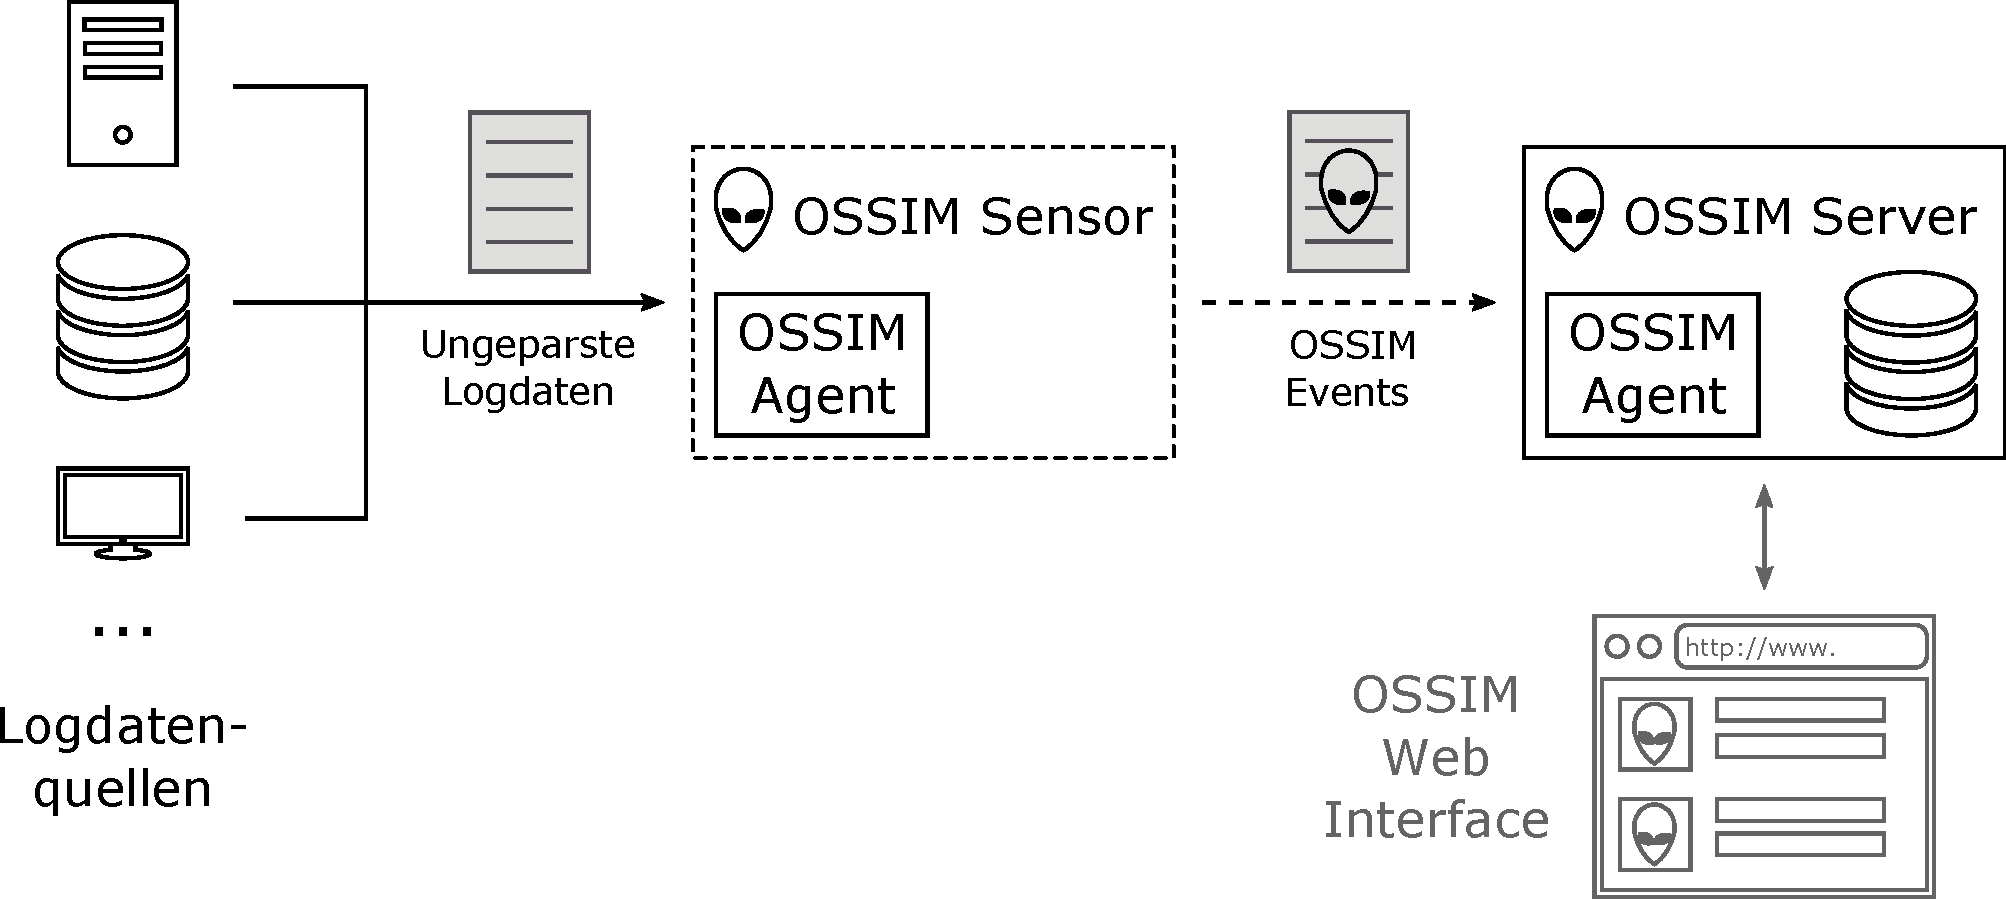
\includegraphics[width=0.9\textwidth]{dia/ossim_log_flow.pdf}
    \caption{High-Level-Übersicht über die OSSIM-Architektur und den Datenfluss.}
    \label{fig:ossim_log_flow}
\end{figure}


\subsection{Parsen von Logdaten in OSSIM}

\label{subsec_state_siem_parsing}

% Quellenarten
% Plugins
% OSSIM-Events
Besonders von Bedeutung für diese Arbeit ist die Verarbeitung von Logdaten. OSSIM ermöglicht es, Logdaten aus unterschiedlichen Quellen entgegenzunehmen bzw. aktiv selber abzurufen und in ein gemeinsames Event-Format zu übersetzen. Hierzu stehen verschiedene Möglichkeiten zur Verfügung:

\begin{itemize}
  \item Entgegennehmen von Daten über das Syslog-Protokoll
  \item Beschaffen von Daten über das SNMP-Protokoll
  \item Entgegennehmen von Daten über proprietäre Protokoll wie SDEE oder WMI
  \item Beschaffen von Daten durch Datenbankabfragen 
\end{itemize}

Unabhängig von der Datenquelle funktioniert die Verarbeitung der Logdaten nach dem immer gleichen Schema. OSSIM bietet die Möglichkeit mitgelieferte oder selber entwickelte Plugins für verschiedene Datenquellen zu aktivieren. Für eintreffende Logdaten überprüft der Agent anhand von regulären Audrücken, ob ein Plugin für das entsprechende Datum zuständig ist. Ist so ein Plugin gefunden, so wird ein neues OSSIM-Event angelegt und anhand der Angaben im Plugin die entsprechenden vorgegebenen Felder des Events gesetzt. Hierbei kann es sich beispielsweise um den Zeitpunkt des Events, IP-Adresse und Port der Datenquelle, einen zu dem Event gehörigen Netzwerkbenutzer oder ereignisabhängige selbstgesetzte Felder handeln. Anschließend folgt die Weiterleitung des Events an den Server.


\section{Pseudonymisierung}

\label{sec_state_pseudonymity}

%pfitzmann2001 - Abschnitt 12
Der Begriff der Pseudonymisierung beschreibt die Benutzung von Pseudonymen zur Identifizierung von Subjekten. Ein Pseudonym (im technischen Sinne) kann nach \cite{pfitzmann2010} als einfache Bitkette betrachtet werden. Es sollte zufällig generiert werden, d.h. vollkommen unabhängig von dem zugehörigen Subjekt oder es betreffenden Eigenschaften sein, um keine Rückschlüsse aus dem Pseudonym selbst zu ermöglichen. Ein Negativbeispiel wäre ein nutzervergebenes Pseudonym, das den Namen des Haustiers enthält. Aber beispielsweise auch eine aufsteigende Nummerierung als Pseudonym könnte durch den hierdurch genauer spezifizierten Erstellungszeitpunkt Rückschlüsse auf das Subjekt hinter dem Pseudonym ermöglichen.

Pseudonymisierung sagt erst einmal lediglich etwas über die Verwendung eines Verfahrens aus, jedoch nichts über die daraus entstehenden Auswirkungen auf die Identifizierbarkeit eines Subjekts oder die Zurechenbarkeit bestimmter Aktionen. Hierfür spielen nach \cite{pfitzmann2001} weitere Eigenschaften von Pseudonymen wie die folgenden eine Rolle:
\begin{itemize}
  \item garantierte Eindeutigkeit von Pseudonymen
  \item Möglichkeit von Pseudonymänderungen
  \item begrenzt häufige Verwendung von Pseudonymen 
  \item zeitlich begrenzte Verwendung von Pseudonymen
  \item Art der Pseudonymserstellung
\end{itemize}

Um die Auswirkungen dieser Eigenschaften einordnen zu können, soll im Folgenden kurz die Pseudonymisierung in zwei Systemen betrachtet und die Relevanz der eben genannten Eigenschaften verdeutlicht werden: Pseudonyme in Mobilfunknetzen und in der Fahrzeug-zu-Fahrzeug-Kommunikation. 

\subsection{Mobilfunknetze}

In Mobilfunknetzen wird zur Identifikation eines Teilnehmers anstelle seiner identifizierenden \textit{International Mobile Subscriber Identity} meist ein Pseudonym -- die \textit{Temporary Mobile Subscriber Identity} (TMSI) -- genutzt, das in bestimmten Situationen gewechselt wird und so Ortung und Bewegungsprofile der Teilnehmer verhindern soll.
In \cite{arapinis2014} beschreiben die Autoren Schwächen der Implementierungen von Mobilfunkstandards in Netzen bei der (Neu-)Vergabe einer TIMSI. Bestimmte Eigenschaften im Bezug auf die Unverkettbarkeit von Pseudonymen und damit auf die Privatsphäre der Nutzer werden in vielen Netzen aufgrund einiger Schwächen nicht erreicht:
\begin{itemize}
  \item Zu seltene Änderung der Pseudonyme
  \item Keine nutzungsabhängige Änderung von Pseudonymen
  \item Pseudonyme werden in verschiedenen Bereichen beibehalten
  \item Anfälligkeit der Neuvergabe für Replay-Angriffe
\end{itemize}
Die letzten beiden Schwächen sind für den Anwendungskontext dieser Arbeit nicht relevant, aber die zeit- und aktivitätsabhängige Neuvergabe von Pseudonymen müssen auch hier beachtet und umgesetzt werden.

\subsection{VANets}

Ein anderer Bereich, der sich besonders mit der Nutzung von Pseudonymen beschäftigt hat, ist die Forschung an Vehicular Ad Hoc Networks (VANets). Hierbei handelt es sich um Netzwerke für die Kommunikation zwischen Fahrzeugen, die beispielweise für die Datenübermittlung zur Bremserkennung naher Fahrzeuge oder die Stauerkennung genutzt werden können. Um die Privatsphäre der Fahrzeughalter zu schützen, wird für die Kommunikation in vielen Ansätzen auf die Verwendung von Pseudonymen gesetzt. So soll sich beispielsweise das Anlegen von Bewegungsprofilen verhindern lassen.\\
Unter anderem in \cite{dotzer2005} und \cite{petit2015} widmen sich die Autoren der Nutzung von Pseudonymen in VANets und den besonderen Anforderungen, die diese erfüllen müssen -- insbesondere auch im Hinblick auf die Häufigkeit von Pseudonymwechseln. Es ergibt sich, dass die Häufigkeit und Situation\footnote{
  Es werden beispielweise Lösungen vorgestellt, die abhängig von Geschwindigkeitsänderungen, einer gewissen Anzahl anderer Fahrzeuge oder besonderen Verkehrssituationen wie Kreuzungen die Pseudonymänderung vornehmen. Das Ziel ist hier immer die Möglichkeit der Pseudonymverkettung bzw. der Bewegungsprofilerstellung durch die äußere Situation der Pseudonymänderung zu erschweren.
}, in der Pseudonymwechsel stattfinden sollten, abhängig vom gewünschten Grad an Anonymität bzw. Angreifermodell sind und außerdem gegenüber Sicherheitsanwendungen\footnote{
  Beispielsweise wäre zur VANet-basierten Kollisionsvermeidung eine Verkettung von Orten, an denen sich ein Fahrzeug zu verschiedenen Zeitpunkten befindet, erstrebenswert.
}  abgewogen werden müssen.\\
Bei der Nutzung von Pseudonymen in VANets handelt es sich natürlich um eine Anwendung mit anders gelagerten Prioritäten im Vergleich zu dem Kontext dieser Arbeit. Dennoch wird deutlich, dass die Strategie zum Pseudonymwechsel stark von der Anwendungssituation abhängig ist. Bezogen auf den hier vorliegenden Anwendungsfall werden insbesondere Besonderheiten der Datenquelle, wie die Häufigkeit von auftretenden Überwachungsdaten, und Anforderungen an die Verknüpfbarkeit von Ereignissen der auf den Daten beruhenden Anomalieerkennung zu beachten sein.

% Perfect Forward Privacy

In \cite{schaub2009} stellt der Autor eine weitere Anforderung an die Nutzung von Pseudonymen in VANets, die jedoch nicht nur für diesen speziellen Anwendungsfall relevant ist: Er verlangt, dass die Aufdeckung eines Pseudonyms keine Informationen über die Identität eines Nutzers im Bezug auf andere Pseudonyme ermöglichen sollte. Diese Eigenschaft bezeichnet er als \textit{Perfect Forward Privacy}\footnote{
  Die Bezeichnung ist an \textit{Perfect Forward Secrecy} angelehnt. Diese Eigenschaft beschreibt ein ähnliches Verhalten bei der verschlüsselten Kommunikation: Ein Angreifer, der in den Besitz des Langzeitschlüssels eines Kommunikationspartners kommt, sollte trotzdem nicht in der Lage sein, bereits aufgezeichnete Nachrichten entschlüsseln zu können.
}.

\subsection{Pseudonymisierung im zu entwickelnden System}

% - Pseudonymgenerierung
% - Pseudonymwechsel zeit und datenmengenabhängig
%   leider nicht genauer, da sowohl datenquellen als auch anomaliedings nicht klar
%   daher parameter ermöglichen
% - PFP in DB umsetzen

Aus diesen Vorüberlegungen können nun die Rahmenbedingungen der in dieser Arbeit verwendeten Pseudonymisierung aufgestellt werden.
Pseudonyme sollten als zufällig gewählte Bitketten hinreichender Länge gewählt werden. Ihre Eindeutigkeit muss sichergestellt werden.

Wie auch in den Beispielen deutlich wurde, müssen Pseudonyme abhängig von dem Anwendungsszenario in bestimmten Fällen für einen Benutzer gewechselt werden. In dem hier vorliegenden Anwendungsfall, in dem Pseudonyme für die Zuordnung von eintreffenden Überwachungsdaten in Unternehmensnetzen genutzt werden, sind insbesondere die Zeitabhängigkeit sowie die Abhängigkeit von der Nutzungshäufigkeit für die Pseudonymwechselstrategie ausschlaggebend. Verschiedene Nutzeraktionen sollten nur in einem gewissen zeitlichen Rahmen und nur in einer gewissen Häufigkeit verkettbar sein. Es handelt sich also um eine schwächere Form der Transaktionspseudonyme, bei der ein Pseudonym je nach Pseudonymwechselstrategie nur für eine bestimmte Anzahl an Ereignissen verwendet wird.

Eine über diese generelle Aussage hinausgehende Bewertung davon, wie diese Abhängigkeiten konkret zu implementieren sind, ist jedoch im Rahmen dieser Arbeit nicht zu leisten. Hierfür sind zwei Gründe ausschlaggebend:
\begin{itemize}
  \item Sie hängen stark von den Eigenschaften der Datenquellen ab, die die Überwachungsdaten liefern. Beispielsweise wäre das Datenprofil, das von einem elektrischen Türschließsystem geliefert wird, sehr unterschiedlich zu dem, das Zugriffe auf einen Netzwerkspeicher protokolliert. Im ersten Fall würden im Allgemeinen selten Daten anfallen, die zudem durch die Anwendung von Hintergrundwissen (Benutzer wird beim Betreten eines Raumes beobachtet) eher zur Aufdeckung eines Pseudonyms führen könnten. Hier wären wahrscheinlich häufige nutzungsabhängige Wechsel angebracht. Eventuell wäre sogar der Extremfall einer einmaligen Pseudonymvergabe pro Aktion in Erwägung zu ziehen.\\
  Im zweiten Fall hingegen würden im Allgemeinen häufig Daten anfallen und erst die Verkettung dieser Daten könnte hilfreiche Rückschlüsse auf vorliegende Anomalien liefern. Ein einzelner Datenzugriff hätte meist wenig Aussagekraft, wohingegen ein massenhafter Zugriff beispielsweise auf die Kundendatenbank eines Unternehmens durch einen gekündigten Mitarbeiter möglicherweise auf Datendiebstahl schließen lassen könnte.
  
  \item Weiterhin muss die Pseudonymwechselstrategie auch abhängig von der später auf den pseudonymisierten Überwachungsdaten auszuführenden automatisierten Anomalieerkennung sein. Je nachdem welche Verfahren auf Daten aus welchen Datenquellen eingesetzt werden sollen, könnte auch hier unterschiedliche Verknüpfbarkeit der Daten erforderlich sein. Hieraus ergibt sich auch ein Spannungsfeld zwischen den Anforderungen der Anomalieerkennung gegenüber der Verknüpfbarkeit der Daten und damit der Privatsphäre der Arbeitnehmer.
\end{itemize}

Aus diesen Gründen wird eine parameterabhängige Pseudonymwechselstrategie implementiert, die sowohl zeit- als auch die nutzungsabhängige Wechsel ermöglicht. Wie lange bzw. häufig ein Pseudonym verwendet wird, kann so in konkreten Anwendungen mit gesetzten Rahmenbedingungen beurteilt und gesetzt werden.
% Digitalgipfel
Dieses Vorgehen wird auch in den \textit{Leitlinien für die rechtssichere Nutzung von Pseudonymisierungslösungen unter Berücksichtigung der Datenschutz-Grundverordnung} beschrieben: \glqq Abhängig vom Anwendungsfall sind – zeit- oder datenvolumenabhängig – geeignete Intervalle zu definieren, in denen ein Wechsel [...] erfolgt.\grqq{}\cite{schwartmann2017}

Weiterhin wird angestrebt für die Pseudonyme bzw. ihre Aufdeckung die erwähnte Perfect Forward Privacy zu ermöglichen. Die konkrete Umsetzung dieser Eigenschaft wird in einem späteren Abschnitt beschrieben werden.

\section{Schwellwertschemata}

\label{sec_state_threshold}

%\subsection{Schemata}

% - RSA signing/decryption \cite{frankel1997proactive} proactive
% - RSA signing/decryption \cite{gennaro1996robust} robust efficient
% - RSA signign/decryption \cite{rabin1998simplified} robust proactive
% - RSA signing \cite{nguyen2005}
% - RSA signing \cite{shoup2000practical}
% - Paillier encryption \cite{damgard2001, fouque2000sharing} -> homomorphic for electronic voting
% - DSS signing \cite{gennaro1996robustdss}
% - Schnorr \cite{stinson2001provably}



Aufbauend auf den Ideen von Shamir und Blakley und den ersten Ideen zu kryptographischen Schwellwertschemata wurden für verschiedene Algorithmen und Anwendungsfälle Schemata mit unterschiedlichen Eigenschaften entwickelt.

\subsection{Übersicht}

Eine Vielzahl von Veröffentlichungen behandlen das Problem der verteilten Erstellung von Signaturen: Die in \cite{shoup2000practical} entwickelte Lösung basiert auf dem RSA-Verfahren, \cite{gennaro1996robustdss} erweitert den DSS-Standard um ein Schwellwertschema und \cite{stinson2001provably} entwickelt ein Schema zur verteilten Signatur mittels Schnorr-Signaturen.\\
Weitere Forschungen haben sich mit der Entwicklung von RSA-basierten Schwellwertschemata zur verteilten Entschlüsselung beschäftigt, die im Kontext dieser Arbeit genutzt werden \cite{frankel1997proactive, gennaro1996robust, rabin1998simplified}. \\
Ein zusätzliches Verfahren, das im Zusammenhang mit verteilter Entschlüsselung Aufmerksamkeit erfuhr, ist das Paillier-Kryptosystem. In \cite{damgard2001} und \cite{fouque2000sharing} entwickelten die Autoren auf diesem System basierte Schwellwertschemata, die insbesondere durch ihre homomorphe Eigenschaft hervorstechen und dadurch im Bereich der elektronischen Wahlsysteme genutzt werden können.\\
Einen Überblick über weitere Veröffentlichungen in diesem Bereich bieten beispielsweise \cite{desmedt1997some}, \cite{gemmell1997} und \cite{desmedt1993}.

\subsection{ElGamal-basiertes Schwellwertschema}

\label{sec_state_threshold_scheme}

Ein Verfahren zur \textit{Threshold Decryption}, das auf auf einer geschickten Kombination von Shamir's Secret Sharing (Abschnitt \ref{sec_basics_threshold_shamir}) und des ElGamal-Kryptosystems (Abschnitt \ref{sec_basics_threshold_elgamal}) basiert, veröffentlichten die Autoren in \cite{DesmedtFrankel1990}. Aufbereitete Darstellungen lassen sich in \cite{katz2014} und \cite{boneh2016} finden. \\
Es ist eines der ersten veröffentlichten Schwellwertschemas und erfuhr dadurch viel Beachtung und entsprechend viele aufbauende Arbeiten, die Verbesserungen vorschlugen. Durch die hinterliegende Mathematik bietet das Schema einfachere Umsetzbarkeit (auch von Erweiterungen wie dezentraler Schlüsselgenerierung) gegenüber RSA\footnote{
  Das ElGamal-Verfahren nutzt zur Berechnung eine öffentlich bekannter Ordnung (sie ist Teil des öffenltichen Schlüssels). Im Gegensatz dazu werden Berechnungen bei RSA in \(\Phi(n)\) ausgeführt, das jedoch nicht öffentlich vorliegen darf \cite{nguyen2005}.
}. Dies gilt ebenso gegenüber den Paillier-basierten Schemata -- deren homomorphe Eigenschaften in dieser Arbeit nicht benötigt werden. Aus diesen Gründen fiel die Wahl des in dieser Arbeit umzusetzenden Schemas auf das genannte Verfahren.\\
Der Rest dieses Abschnitts stellt das Verfahren nun entsprechend den in Abschnitt \ref{sec_basics_threshold_thresholddecryption} aufgeführten Algorithmen eines Threshold-Public-Key-Decryption-Systems im Detail vor.

%\subsection{Umzusetzendes kryptographisches Schwellwertschema}

%- Desmedt und Frankel, aufbereitet auch in Katz und Boneh.

%- Verfahren basierend auf Shamir und ElGamal

%- Analog zu basics-threshold-formal (zentrale) lässt sich das Verfahren in 4 Phasen unterteilen

\textbf{Algorithmus G: Schlüsselgenerierung}

In dem Verfahren wird für die Schlüsselgenerierung eine zentrale, vertrauenswürdige Instanz vorausgesetzt, die den öffentlichen Schlüssel und die später benötigten Shares des geheimen Schlüssels erzeugt und verteilt. 

Zur Erzeugung werden zwei Primzahlen \(p\) und \(q\) mit der Eigenschaft \(p = 2q + 1\) - bekannt als sichere Primzahl bzw. Sophie-Germain-Primzahl - benötigt. Weiterhin ist ein Generator der Untergruppe der Ordnung \(q\) von \(\mathbb{Z}_p^*\) notwendig.

Der (temporär erstellte) geheime Schlüssel \(a \in \mathbb{Z}_q\) wird analog zu der Schlüsselgenerierung im ElGamal-Verfahren zufällig gewählt. Aus ihm wird der öffentliche Schlüssel \(pk = g^a \mod p\) berechnet.\\
Der geheime Schlüssel wird anschließend analog zu Shamirs Secret Sharing in \(\mathbb{Z}_q\) in einzelne Shares \((x_i, y_i) = (x_i, q(x_i))\) aufgeteilt und diese an die Teilnehmer verteilt. Anschließend werden diese Werte gelöscht, so dass nur noch die Teilnehmer im Besitz ihrer Shares und damit in der Lage sind, Schlüsseltexte zu entschlüsseln.

\textbf{Algorithmus E: Verschlüsselung}

Anschließend kann ein Klartext mithilfe von \(pk\) analog zu dem ElGamal-Verfahren 
%(siehe Abschnitt \ref{sec_basics_threshold_elgamal}) 
verschlüsselt werden. So erhält man \((v,c) = (g^k, m \cdot g^{ak})\) für ein durch den Sender zufällig gewähltes \(k \in \mathbb{Z}_q\).

\textbf{Algorithmus D: Partielle Entschlüsselung}

Jeder Besitzer eines Shares \((x_i, y_i)\) kann nun für den zu entschlüsselnden Schlüsseltext \((v,c)\) seine partielle Entschlüsselung \((x_i, v^{y_i})\) berechnen und diese an eine zentrale Instanz, den Combiner, senden. Empfängt dieser mindestens \(t\) partielle Entschlüsselungen\footnote{
  Zur Erinnerung: \(t\) beschreibt die Mindestzahl zur Entschlüsselung benötigter Shares des Schwellwertschemas.
}, so kann er den Klartext wiederherstellen.

\textbf{Algorithmus C: Kombination}

Hierzu berechnet der Combiner die Lagrange-Koeffizienten \(\lambda_i \in \mathbb{Z}_q\) wie in Shamir's Secret Sharing beschrieben\footnote{
  In diesem Abschnitt gilt \(i \in C\). \(C\) stellt dabei die Menge der Indizes der beteiligten Sharebesitzer dar. Es gilt also \(C \subseteq \{1, \dots, n\}\) und \(| C | \ge t\).
}. Anschließend kann
 
\[g^{ak} = \prod_{i=1}^k (v^{y_i})^{\lambda_i}\]

berechnet werden. Dies funktioniert, da 

\[
\prod_{i=1}^k (v^{y_i})^{\lambda_i} = 
\prod_{i=1}^k (g^k)^{y_i \cdot \lambda_i} = 
(g^k)^{\sum_{i=1}^{k} y_i \cdot \lambda_i} \overset{(*)}{=}
(g^k)^a
\]

gilt. Der letzte Schritt \((*)\) folgt direkt aus dem zugrundeliegenden Secret-Sharing-Schema und ist in dieser Form bereits in Abschnitt \ref{sec_basics_threshold_shamir} zu finden.

Anschließend kann der Klartext als \(m = c \cdot (g^{ak})^{(-1)}\) wiederhergestellt werden. 

\subsection{Verteilte Schlüsselgenerierung}

\label{sec_state_threshold_distributed}

Ein Nachteil dieses Verfahrens in der Phase der Schlüsselgenerierung ist, dass für die Generierung des geheimen Schlüssels und der daraus resultierenden Shares eine zentrale und vertrauenswürdige Instanz notwendig ist. Diese Problematik wurde bereits in Abschnitt \ref{subsec_impl_requirements_threshold} dargestellt und Auswirkungen in Abschnitt \ref{subsec_impl_requirements_attackermodel} betrachtet.

In \cite{pedersen1991} wurde vom Autor eine Möglichkeit der verteilten Schlüsselgenerierung für das dargestellte Verfahren vorgeschlagen, die von den Autoren in \cite{gennaro1999} noch verbessert wurde. 

Das Verfahren besteht aus zwei Phasen: In der ersten Phase wird von allen potentiellen Share-Besitzern ein \textit{Verifiable Secret Sharing Scheme}\footnote{
  Verifiable Secret Sharing Schemes sind Secret Sharing Schemes, die es den Share-Besitzern erlauben zu überprüfen, ob ihre Shares konsistent sind, d.h. ob es möglich ist aus den Shares ein gemeinsames Geheimnis wiederherzustellen. Bei dem in Abschnitt \ref{sec_basics_threshold_shamir} vorgestellten Secret Sharing nach Shamir ist dies beispielsweise nicht der Fall. Ein bösartiger Erzeuger von Shares könnte für jeden Beteiligten ein anderes Geheimnis benutzen, so dass bei der Rekonstruktion abhängig von beteiligten Share-Besitzern unterschiedliche Geheimnisse erhalten werden.
} (VSS) nach Pedersen ausgeführt, das dafür sorgt, dass anschließend alle ehrlichen Beteiligten jeweils im Besitz eines Shares sind, die zusammengenommen den geheimen Schlüssel \(x\) bilden (der jedoch nirgendwo vorliegt oder im Laufe des Verfahrens vorlag). In der zweiten Phase wird ein VSS nach Feldman dazu genutzt, den gemeinsamen öffentlichen Schlüssel \(y = g^x\) auf eine Weise zu berechnen, die wiederum dafür sorgt, dass der geheime Schlüssel nirgendwo vorliegen muss. Auf diese Weise wird die vertrauenswürdige Instanz vermieden und es ist trotzdem sichergestellt, dass die ehrlichen Beteiligten im Besitz von Shares sind, die die Verwendung des kryptographischen Schwellwertschemas so ermöglichen wie im letzten Abschnitt für das Verfahren mit zentraler Schlüsselgenerierung vorgestellt.

\subsection{ECC-ElGamal}

\label{sec_state_threshold_ecc}

Eine andere Verbesserung für das Verfahren ist die Verwendung von \textit{Elliptic Curve Cryptography}. Hier werden die Berechnungen des ElGamal-Verfahrens nicht mehr in der beschriebenen Untergruppe von \(\mathbb{Z}_p^*\), sondern als Operationen auf elliptischen Kurven über endlichen Körpern ausgeführt \cite{koblitz1987elliptic}.

Vorteil der Verwendung ist eine deutlich geringere benötigte Schlüssellänge für vergleichbare Sicherheit im Vergleich zu dem ursprünglichen Verfahren\footnote{
  Das BSI gibt eine Schlüssellänge von etwa 250 Bits für ECC-Verfahren als vergleichbare Sicherheit erreichend zu 2000-Bit-Schlüsseln für Verfahren wie RSA oder auf dem Diskreten-Logarithmus-Problem beruhenden Verfahren an \cite{bsi2018}.
}. Durch diese kürzeren Schlüssel werden auch Berechnungszeit und Speicherverbrauch trotz komplexerer Berechnungen eingespart werden.

\subsection{Verallgemeinerte Schwellwerte}

\cite{ito1989secret} \textit{Access structure}
\todo{Schreiben!}

\subsection{Existierende Implementierungen}

\label{sec_state_threshold_existing_impl}

Auch nach umfangreicher Recherche ließ sich keine quelloffene, kryptographisch überprüfte und lizenzrechtlich nutzbare Bibliothek finden, die das gewünschte Schwellwertschema implementiert. Es gab verschiedene verwandte Lösungen wie Civitas\footnote{
  Civitas -- A secure voting system. http://www.cs.cornell.edu/projects/civitas/
} oder Helios\footnote{
  Helios Voting. https://heliosvoting.org/
}, die jedoch alle eng mit dem Anwendungskontext der elektronischen Wahl verknüpft waren und dadurch andere Anforderungen erfüllten als sie für diese Arbeit erforderlich sind. Aus diesem Grund wird das beschriebene Schwellwertschema gezwungenermaßen in Teilen selbstständig implementiert.

\section{Searchable Encryption}

\todo{To be written...}

\chapter{Implementierung}


\begin{itemize}
  \item \textbf{Anforderungen} Welche Anforderungen muss der Prototyp erfüllen?
  \item \textbf{Umsetzung} Architektur und Implementierung des Prototypen.
  \item \textbf{Einbindung in OSSIM} An welcher Stelle wird er in das SIEM-System integriert? Abwägung der verschiedenen Möglichkeiten.
  \item \textbf{Umsetzung des Schwellwertschemas} Implementierung des Schwellwertschemas und Integration in den Prototypen. Hier auch Key Management.
\end{itemize}


\label{cha_implementation}



\section{Anforderungen}

\label{sec_impl_requirements}

Der umgesetzte Prototyp soll es ermöglichen, aufbauend auf dem bestehenden Open-Source-SIEM-System OSSIM Logdaten mittels Pseudonymisierung und Schwellwertschemata so zu verändern, dass diese erst durch Kollaboration einer bestimmten Anzahl an Teilnehmern wieder aufgedeckt werden können. Neben dieser primären Anforderung sollte er noch weitere wie die Erweiterbarkeit um weitere Dateschutztechniken erfüllen. Alle diese Anforderungen sollen im folgenden Abschnitt näher erläutert werden. Zuerst wird jedoch ein Angreifermodell für die prototypische Umsetzung aufgestellt.

\subsection*{Zugrundeliegendes Angreifermodell}

% Das Angreifermodell definiert die	maximal	berücksichtigte	Stärke eines Angreifers, gegen den ein	Schutzmechanismus	gerade noch wirkt.	
%Es beschreibt:
%–  Rollen des Angreifers (Außenstehender, Benutzer, Betreiber, Wartungsdienst, Produzent, Entwerfer …), auch kombiniert 
%–  Verbreitung des Angreifers (Stellen im System, an denen der Angreifer Informationen gewinnen oder Systemzustände verändern kann) 
%–  Verhalten des Angreifers 
%  •  passiv / aktiv,  beobachtend / verändernd 
%–  Rechenkapazität des Angreifers 
%  •  unbeschränkt: informationstheoretisch 
%  •  beschränkt: komplexitätstheoretisch 

Im Kontext dieser Arbeit, die sich mit der datenschutzfreundlichen Speicherung von Überwachungsdaten beschäftigt, muss zuerst folgende Vorüberlegung getroffen werden: Logdaten erreichen das verwendete SIEM-System abhängig von den verwendeten Protokollen im allgemeinen nicht-pseudonymisiert und oftmals weder verschlüsselt noch mit geschützer Integrität über das Netzwerk. \todo{Angriffsmöglichkeiten erläutern: Mitschneiden aller Daten und damit  Aufdecken von Pseudonymen, ...}
Diese Angriffsmöglichkeiten zu verhindern, ist ausdrücklich kein Ziel dieser Arbeit. Daher bezieht sich das Angreifermodell auf die Bearbeitung und Speicherung von Logdaten, erst sobald sie das zu entwickelnde System erreichen, jedoch nicht vorher.

Das Ziel des Systems bezogen auf seine Sicherheit lässt sich folgendermaßen definieren: Das Pseudonym eines Nutzers erlaubt (ohne Anwendung von Hintergrundwissen) keinen Rückschluss auf die Identität eines Nutzers. Erst die Kollaboration berechtigter Akteure ermöglicht das Aufdecken eines Pseudonyms.\todo{? außerdem erweitern um aktive Angreifer?}

Ein Angreifermodell beschreibt die maximale Stärke eines Angreifers im Bezug auf verschiedene Faktoren, gegen die ein System abgesichert ist. Enthalten sind die Rolle eines Angreifers, seine Verbreitung im System, aktives oder passives Verhalten und die Rechenkapazität, die der Angreifer zum Überwinden der eingesetzten Schutzmaßnahmen aufbringen kann. Es bildet die Basis für alle Folgeüberlegungen im Bezug auf die Sicherheit des zu entwickelnden Systems.

Für das Angreifermodell werden folgende Annahmen getroffen: Bei dem Angreifer kann es sich um einen Außenstehenden, um einen Berechtigten mit Zugriff auf das SIEM-System oder sogar um einen Administrator mit physischem Zugriff auf Rechner im Netz handeln. Wie bereits beschrieben, wird die ungesicherte Übertragung nicht-pseudonymisierter Daten zu dem System nicht betrachtet. Insofern wird von einem Angreifer ausgegangen, der erst Zugriff auf das zu entwickelnde System oder das SIEM-System beseitzt oder erlangt. Das zu entwickelnde System soll in der Lage sein, sich auch gegen aktive Angreifer zur Wehr zu setzen. \todo{Denial of Service etc?}
Bezogen auf die verfügbare Rechenleistung des Angreifers sollen verbreitete und nach heutigem Wissensstand für sicher befundene kryptographische Algorithmen als nicht mit vertretbarem Aufwand zu brechen angesehen werden. Es handelt sich daher um die Annahme von komplexitätstheoretischer Sicherheit.


\subsection*{Anforderungen an die Integration in OSSIM}

\label{sec_requirements_ossim_integration}

Um zu beurteilen, an welcher Stelle in den Datenfluss der Logdaten in OSSIM (vergleiche Abschnitt \ref{sec_state_siem}) eingegriffen wird, um die Daten zu verändern, müssen Vor- bzw. Nachteile der verschiedenen Möglichkeiten gegeneinander abgewogen werden. Folgende Eigenschaften einer Möglichkeit sollten betrachtet werden:

\begin{itemize}

  \item \textbf{Abhängigkeit von der OSSIM-Konfiguration: } Ist die Lösung sowohl in der verteilten als auch in der All-in-One-Installation von OSSIM umsetzbar? Eine Lösung, die unabhängig von der gewählten Installationsmethode funktioniert, ist zu bevorzugen, da sie universell einsetzbar ist.
  
  \item \textbf{Veränderung des SIEM-Systems: } Muss OSSIM für die Umsetzung der Lösung verändert werden? Dies wäre im Hinblick auf zukünftige Updates, die OSSIM durch den Entwickler erfährt, nicht wünschenswert, da jedes dieser Updates dafür sorgen könnte, dass die umgesetzte Lösung angepasst werden muss. Hierbei können sowohl direkte Änderungen an dem OSSIM-Quellcode als auch Eingriff in die interne Kommunikation betrachtet werden.  
  
  \item \textbf{Nicht-pseudonymisierte Daten im SIEM-System: } Um das Ziel der Arbeit - die Pseudonymisierung, die nur durch Kollaboration aufgedeckt werden kann - zu erreichen, muss sichergestellt sein, dass Logdaten nirgendwo in nicht pseudonymisierter Form vorliegen. Da insbesondere das zukünftige Verhalten von OSSIM nicht beeinflusst werden kann, wäre es wünschenswert, dass die Logdaten bereits in pseudonymisierter Form das SIEM-System erreichen.\\
  Die Relevanz dieser Eigenschaft lässt sich bereits an einem einfachen Beispiel erkennen: Wird das Syslog-Protokoll genutzt, um Logdaten in OSSIM aufzunehmen, so werden die Einträge im Sensor erst in eine Logdatei gespeichert und von dort aus geparst, normalisiert und in der Datenbank gespeichert. Das Datum verbleibt in der Logdatei. Kommen die Daten in nicht-pseudonymisierter Form in dem OSSIM-Sensor an, so muss sichergestellt werden, dass verarbeitete Einträge gelöscht/verändert werden.
  
  \item \textbf{Mehrfaches Parsen von Logdaten: } Durch den OSSIM-Agenten werden die Logdaten - wie in Abschnitt \ref{sec_state_siem} beschrieben - geparst und normalisiert. Aus Performancegründen ist eine Lösung zu bevorzugen, die dieses Parsen nicht mehrfach voraussetzt.
  
%  \item \textbf{Manipulierbarkeit auf den Übertragungswegen(?): }

\end{itemize}

\subsection*{Anforderungen an die Pseudonymisierung}

%- Lang genug für geringe Kollisionswsk.
%- Eindeutig
%- Durchsuchbar (mim Hinblick auf threshold)
%- Anwendungsfallabhängige Parameter für Nutzzeit, ... (Rückblick auf Kapitel 3)

Die Pseudonymisierung muss es ermöglichen nach Aufdecken eines Eintrags wieder auf den ursprünglichen Dateninhalt schließen zu können. Daher müssen die Pseudonyme für die Zeit ihrer Speicherung eindeutig sein, d.h. es darf zu keiner gleichzeitigen Mehrfachverwendung von Pseudonymen kommen. 

Weiterhin muss es eine Möglichkeit beim Pseudonymisieren von Logeinträgen geben, zu überprüfen, ob für ein Datum bereits ein Pseudonym vergeben wurde. So kann sichergestellt werden, dass in einem bestimmten Zeitraum Logeinträge zu einer Person mit dem gleichen Pseudonym versehen werden, um über die Verknüpfung von Einträgen die gewünschte Erkennung von Insider-Angriffen erreichen zu können.

Außerdem muss es eine Möglichkeit geben, die Parameter der Pseudonymisierung wie den Zeitraum ihrer Verwendung (vergleiche Abschnitt \ref{sec_state_pseudonymity}) konfigurierbar zu machen.

\subsection*{Anforderungen im Bezug auf den Einsatz eines kryptographischen Schwellwertschemas}

%- Verteiltes Modell 
%- Kommunikation
%- Schlüsselmanagement
%- ...

\todo{Anpassen nach Kapitel 3 - Threshold-Abschnitt?}

Der Einsatz eines kryptographischen Schwellwertschemas setzt eine verteilte Anwendung voraus, die den Zugriff für die Pseudonymisierungskomponente sowie für die bei der Entschlüsselung eines Eintrags beteiligten Akteure bereitstellt. Die für das Schwellwertschema nötigen Parameter \(t\) und \(n\) sowie die beteiligten Akteure müssen anpassbar bzw auswählbar sein.

In der Phase der Schlüsselgenerierung muss das System die Kommunikation und Koordination aller Beteiligten unterstützen. Die hier erstellten Schlüssel und \textit{Shares} müssen an geeigneten Stelle sicher gespeichert und abrufbar sein.

Der für die Verschlüsselung erforderliche öffentliche Schlüssel muss so vorliegen, dass er bei der Verschlüsselung eines Pseudonym-Datensatzes genutzt werden kann.

Bei der Entschlüsselung eines Eintrags, also der Aufdeckung eines Pseudonyms, muss das System wiederum die beteiligten Aktuere koordinieren und anschließend die Rolle des \textit{Combiners} übernehmen, so dass anschließend der entschlüsselte Datensatz zentral vorliegt.

\subsection*{Benutzerinteraktion}

%- Proxy: Konfiguration der Plugins

%- Pseudo-App: Statusanzeige angemeldeter Benutzer(Admin), Initialisierung der Schlüsselgenerierung nach Nutzerauswahl(Admin), Anlegen von Aufdeckanfragen, Statusanzeige von Aufdeckanfragen, Systemstatus

%- Einzelne Teilnehmer sollten Client-Anwendungen besitzen, um auf Anfragen reagieren zu können (Generation eigener Schlüssel, gemeinsame Schlüsselgenerierung, ... ) Konsolenanwendung? 

Die zu entwickelnde verteilte Anwendung wird an verschiedenen Stellen Benutzerinteraktion erfordern.

Das Konfigurieren des Systems zur Integration verschiedener Datenquellen und deren Beschreibung muss einem berechtigten Nutzer zugänglich gemacht werden. Ebenso sollte es im Hinblick auf die in der Aufgabenstellung geforderte Erweiterbarkeit im Bezug auf weitere Datenschutztechniken relativ leicht sein, diese Techniken im System nutzen zu können. 

Für pseudonymisierte Datensätze muss es berechtigten Benutzern ermöglicht werden, Anfragen zur Aufdeckung eines Pseudonyms zu stellen und sich über ihren Status informiert zu halten.

Für die Benutzung eines kryptographischen Schwellwertschemas sollte es einem Administrator des Systems ermöglicht werden, grundlegende Parameter des Systems wie die Schwellwertparameter und die beteiligten Nutzer auszuwählen sowie die Initialisierung des Schemas anzustoßen. \\
Die am Schwellwertschema beteiligten Nutzer müssen die Möglichkeit erhalten, eine Übersicht über sie betreffende Anfragen zur Aufdeckung eines Pseudonym-Datensatzes zu bekommen sowie einzelne Anfragen abzulehnen oder sich an m Prozess des Aufdeckens mithilfe des Schwellwertschemas zu beteiligen. 

\todo{Performance?}

\subsection*{Erweiterbarkeit um neue Datenquellen}

Das umzusetzende System sollte es ermöglichen, Daten aus verschiedenen Quellen und (abhängig vom gewählten Eingriffspunkt in OSSIM auch) in verschiedenen Formaten entgegenzunehmen und mithilfe der umgesetzten Datenschutztechniken verändern zu können. Dabei muss das Format der Logdaten grundsätzlich beibehalten werden, um die Behandlung der Daten in OSSIM weiterhin zu ermöglichen.

\subsection*{Erweiterbarkeit um neue Datenschutztechniken}

Neben der im Fokus dieser Arbeit stehenden Pseudonymisierung und dem Einsatz von kryptographischen Schwellwertschemata zum Schutz der Logdaten gibt es weitere Datenschutztechniken, die für den Anwendungsfall genutzt werden könnten (siehe Kapitel \ref{cha_alternatives}). Der umgesetzte Prototyp sollte leicht um diese Techniken erweiterbar sein, d.h. so gestaltet sein, dass andere Techniken ohne große Änderungen am System integriert und auf eingehende Logdaten angewendet werden können.



\section{Entwurf}

\label{sec_impl_architecture}

\todo{Einführender Absatz}

\subsection{Eingriff in den OSSIM-Datenfluss}

\todo{Hier oder in Anforderungen?}

Für den Eingriff zur Pseudonymisierung der Logdaten bieten sich verschiedene Stellen im Datenfluss von OSSIM an. In diesem Abschnitt sollen die verschiedenen Möglichkeiten dargestellt und gegeneinander abgewogen werden. Eine Übersicht über die verschiedenen Stellen bietet Abbildung \ref{fig:ossim_data_access_point}. Im Folgenden sollen die verschiedenen Möglichkeiten bezogen auf die in Abschnitt \ref{subsec_impl_requirements_ossimintegration} dargestellten Eigenschaften bewertet werden.

\begin{enumerate}

\item \textbf{In der Quelle der Logdaten}\\
  Bei diesem Ansatz werden die Daten bereits pseudonymisiert, bevor sie die Datenquelle verlassen. Auch wenn dieser Ansatz aus datenschutztechnischer Sicht die beste Möglichkeit darstellen würde, so ist er doch nicht umsetzbar, da hierzu jede mögliche Quelle von Logdaten universell verändert werden müsste.

\item \textbf{Syslog-Proxy}\\
  Dieser Ansatz pseudonymisiert die Daten vor dem ersten Kontakt mit einer OSSIM-Komponente, indem Datenquellen ihre Logdaten an einen Proxy senden, der die Daten pseudonymisiert und erst anschließend an OSSIM weiterreicht. Hierdurch wird erreicht, dass die Daten zu keiner Zeit nicht-pseudonymisiert in OSSIM vorliegen. Ein Nachteil dieser Lösung ist, dass sie das Parsen und Neuzusammensetzen der Logdaten im Proxy erfordert. \todo{Beschreibung erweitern - analog zu Plugins in OSSIM}

\item \textbf{Patchen des OSSIM-Sensor-Agents}\\
  Bei dieser Lösung müsste der OSSIM-Agent des Sensors so verändert werden, dass vor dem Senden der Events an den Server die Pseudonymisierung stattfindet. Daten erreichen den OSSIM-Server nur pseudonymisiert und mehrfaches Parsen wie in der zweiten Lösung wird verhindert. Auf der anderen Seite erfordert diese Lösung einen Eingriff in die Funktionsweise von OSSIM, was beispielsweise bei Updates von OSSIM zu Problemen führen kann. Außerdem liegen die Daten zu Beginn in nicht-pseudonymisierter Form im Sensor vor. \todo{Syslog-Problematik erwähnen} Zusätzlich erfordert diese Lösung die verteilte Installation von OSSIM-Sensor und -Server, schließt also die All-In-One-Installation aus.
  
\item \textbf{Sensor-Server-Proxy}\\
  Hier wird ein Proxy zwischen Sensor und Server geschaltet, der bereits geparste Events pseudonymisiert und anschließend an den Server sendet. Dieser Ansatz würde mehrfaches Parsen verhindern und dafür sorgen, dass nur pseudonymisierte Logdaten den OSSIM-Server erreichen. Wie die vorhergehende Lösung würde er jedoch nur in der verteilten Installation funktionieren und zusätzlich in die Kommunikation zwischen Sensor und Server aktiv eingreifen, was im Hinblick auf die Nachrichtenintegrität\footnote{
    In der aktuellen Version von OSSIM werden Nachrichten unverschlüsselt und nicht signiert zwischen Sensor und Server versendet, aber zu hoffen ist, dass dieser Zustand sich in zukünftigen Versionen noch ändert.
  } und auch auf geändertes Verhalten nach Updates von OSSIM einen Nachteil darstellt.
  
\item \textbf{Patchen des OSSIM-Servers}\\
  Die letzte Möglichkeit ist das Verändern des OSSIM-Servers selbst. Diese Lösung ist vergleichbar mit der dritten Möglichkeit. Zusätzlich würde sie bei der verteilten sowie bei der All-In-One-Installation funktionieren, auf der anderen Seite aber zulassen, dass nicht-pseudonymisierte Events sogar noch direkt auf dem Server vorliegen.

\end{enumerate}

\begin{figure}[]
    \centering
        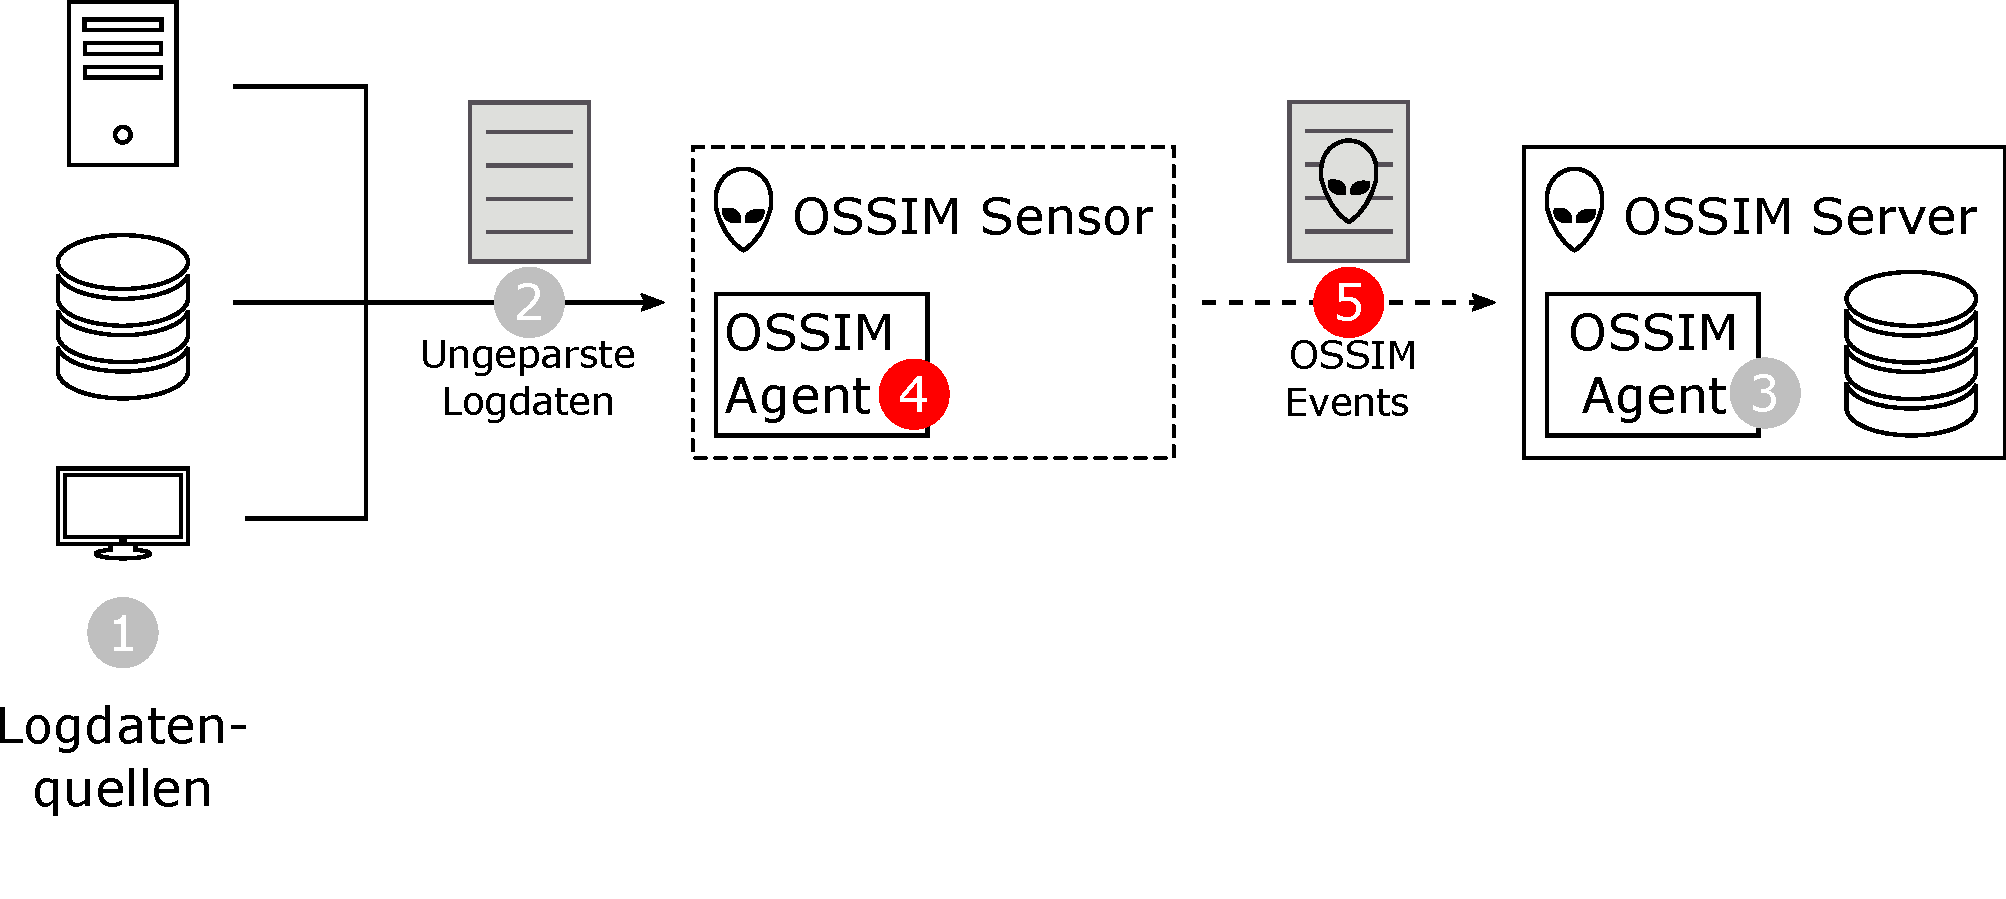
\includegraphics[width=0.9\textwidth]{dia/ossim_data_access_point.pdf}
    \caption{Mögliche Eingriffspunkte in den OSSIM-Datenfluss.}
    \label{fig:ossim_data_access_point}
\end{figure}

Insbesondere der aus datenschutztechnischer Sicht relevante Vorteil, dass die Daten bereits pseudonymisiert in allen OSSIM-Komponenten eintreffen, ließ die Entscheidung auf die \textbf{zweite Möglichkeit} fallen. Dass die Lösung außerdem noch für beide Varianten der OSSIM-Installation möglich ist und keine Anpassungen an OSSIM selbst benötigt, wiegt den Nachteil des zusätzlichen Parsens und wieder Zusammensetzens der Lognachricht bei Weitem auf.\todo{Auch auf Angreifermodell beziehen}





\subsection{Architektur}

%- Beschreibung Architektur
%
%- Wie deckt dieser Ansatz die Anforderungen ab?
%  - Einbindung OSSIM
%  - Pseudonymisierung
%  - Schwellwert
%  - Benutzerinteraktion
%  - Erweiterbarkeit Datenquellen
%  - Erweiterbarkeit Datenschutztechniken

Ausgehend von diesen Überlegungen wurde ein verteiltes System entworfen, dass die Anforderungen aus Abschnitt \ref{sec_impl_requirements} erfüllt und an der beschriebenen Stelle in den Datenfluss eingreift. 
Einen Überblick bietet Abbildung \ref{fig:high__level_architecture}. Das System besteht aus verschiedenen Komponenten, die im Folgenden näher beschrieben werden.

\begin{figure}[]
    \centering
        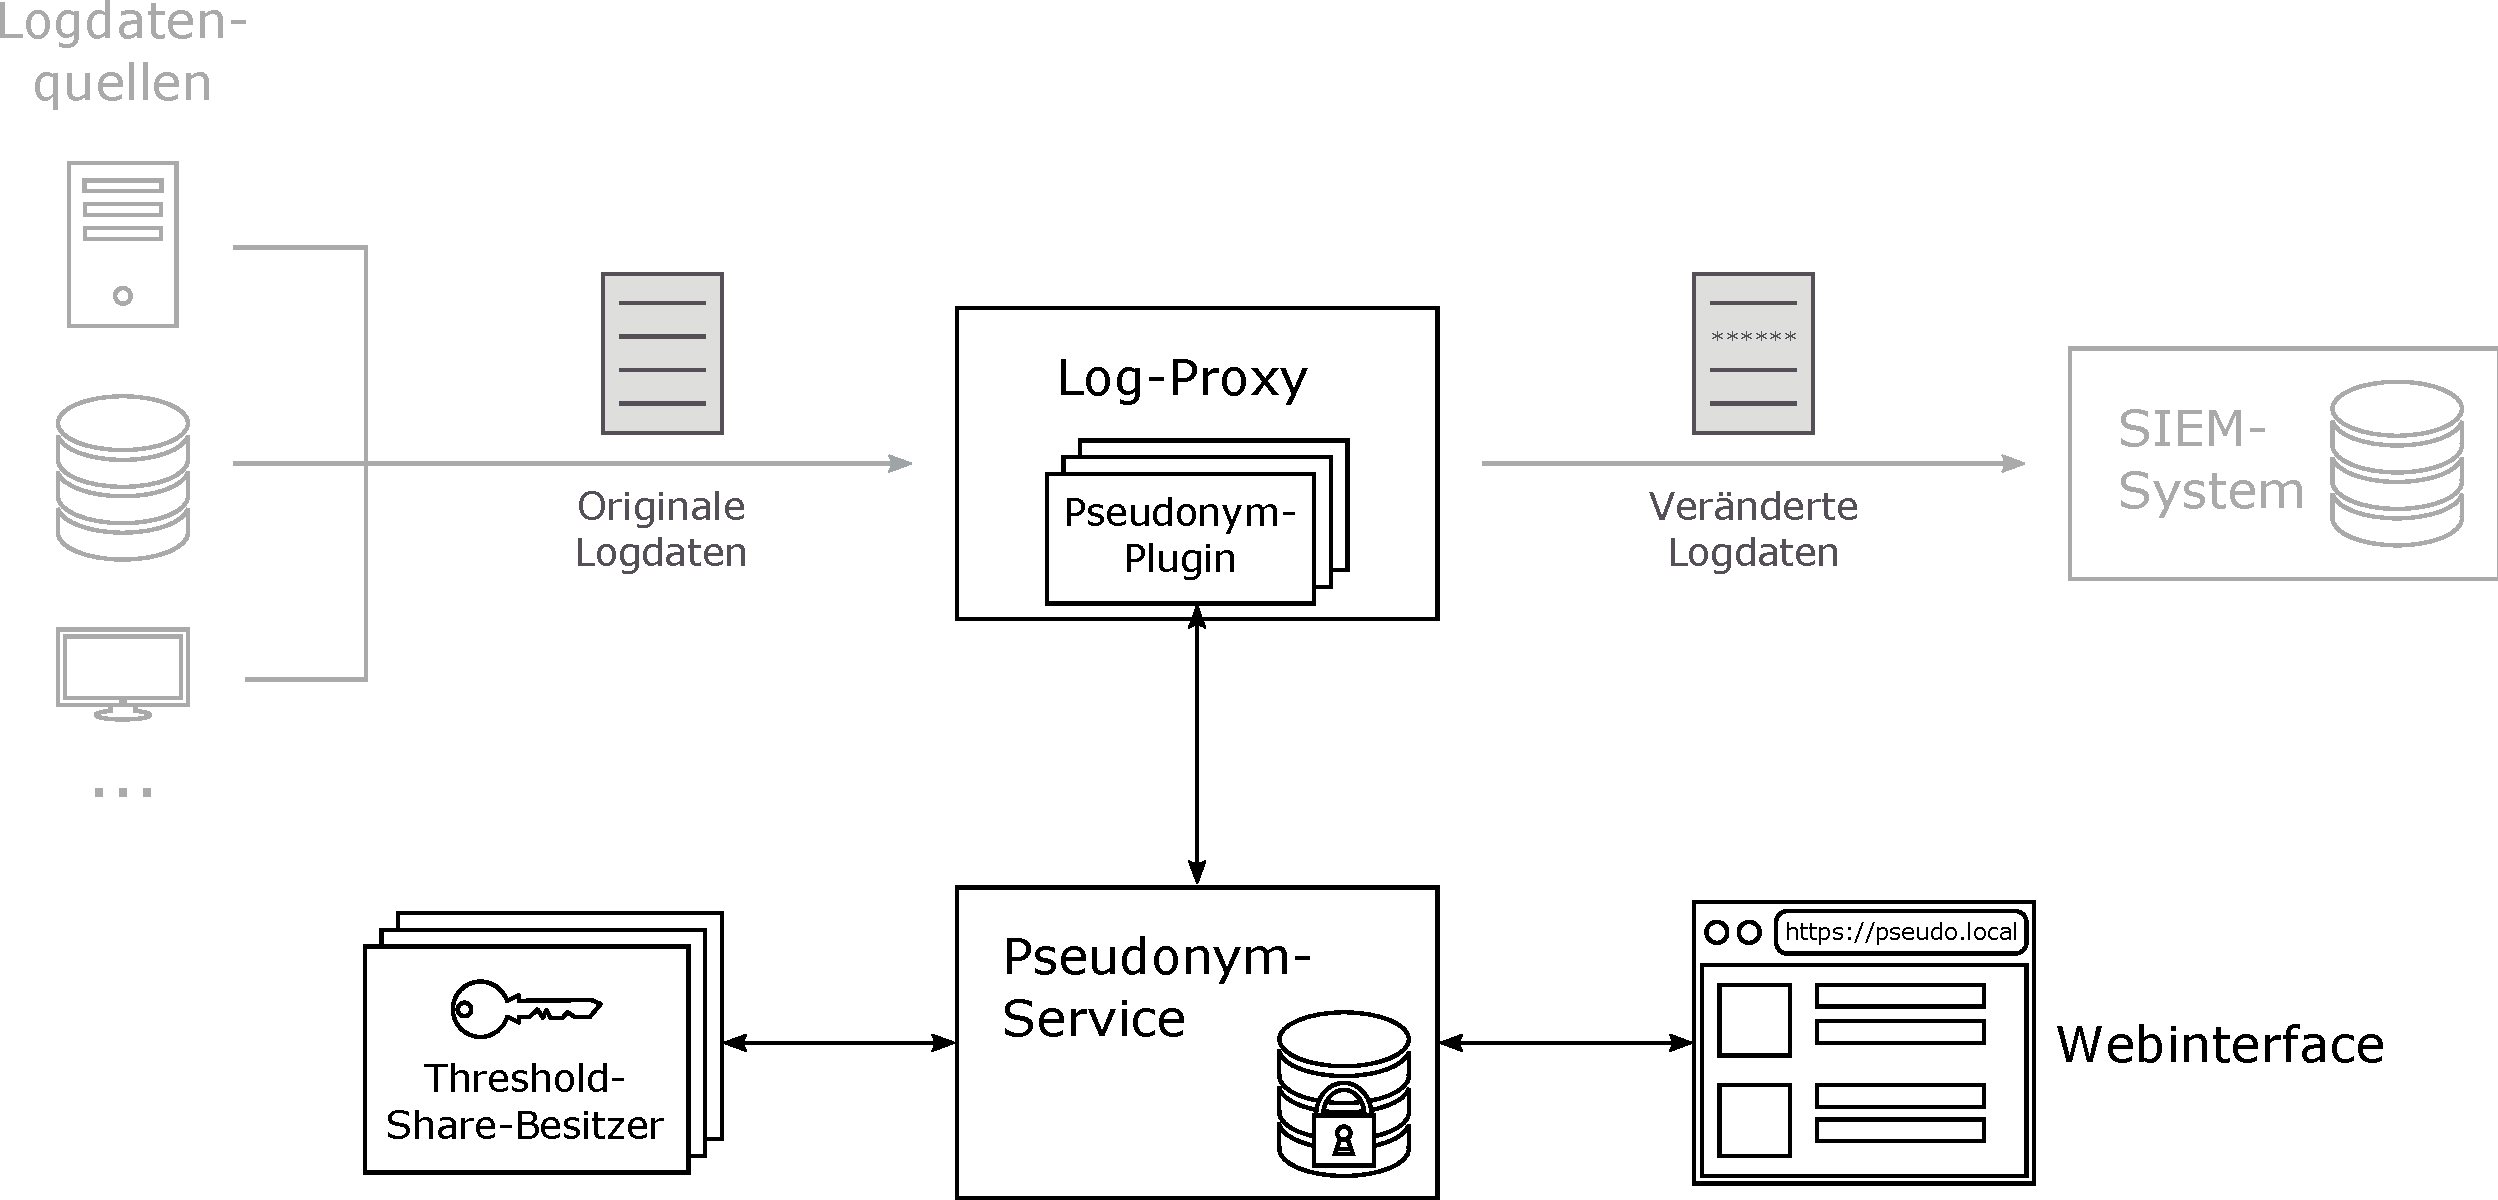
\includegraphics[width=0.9\textwidth]{dia/high_level_architecture.pdf}
    \caption{Ein Überblick über die entworfene Architektur.}
    \label{fig:high__level_architecture}
\end{figure}
\todo{Change Store to Service, Webinterface, Log-Proxy}

Ein \textbf{Log-Proxy}, der die Daten über das Syslog-Protokoll entgegennimmt, verändert und anschließend an OSSIM weiterleitet. Das Verändern der Daten kann mit verschiedenen Plugins geschehen, so dass neben der umzusetzenden Pseudonymisierung auch weitere Datenschutztechniken eingesetzt werden können, was die geforderte Erweiterbarkeit aus Abschnitt \ref{subsec_impl_requirements_plugins} ermöglicht. Der Proxy leistet die Behandlung von Logdaten aus verschiedenen Quellen (siehe Abschnitt \ref{subsec_impl_requirements_differentsources}), was wie bereits im vorhergehenden Abschnitt beschrieben durch Parsen und Wiederzusammensetzen der Daten geschehen muss. Die Konfiguration des quellenabhängigen Vorgehens bei der Logdatenverarbeitung erfolgt ebenfalls hier.

Ein in dem Proxy enhaltenes Plugin wird für die Pseudonymisierung von Daten zuständig und kommuniziert dazu mit einer externen Komponente -- dem Pseudonym-Service. Die Kommunikation mit dem Proxy erfolgt über einen Webservice-basierten Ansatz. Das Plugin kann für eingehende Daten ein Pseudonym anfordern und dieses anschließend in den Logdaten verwenden.

Der \textbf{Pseudonym-Service} erfüllt zwei Aufgaben: das Speichern und Verwalten der Pseudonyme sowie die Integrierung des kryptographischen Schwellwertschemas. Initial muss die Schlüsselgenerierung des Schwellwertschemas (bei zentraler Schlüsselgenerierung) oder die Koordinierung der teilnehmenden Benutzer (bei dezentraler Schlüsselgenerierung) durch den Service geleistet werden. 
Es können während des Betriebs neue Pseudonyme angelegt und zusammen mit ihrem durch das Schwellwertschema verschlüsselten Datum abgelegt werden. Sie werden durch geeignete Maßnahmen durchsuchbar gehalten, um für ein Datum überprüfen zu können, ob bereits ein Pseudonym vergeben wurde. 
Über ein Webinterface kann ein berechtiger Benutzer die Aufdeckung eines bestimmten Pseudonyms fordern und den Status seiner Forderung bzw. im Erfolgsfall das aufgedeckte Datum betrachten. Dieses Datum wird durch das Kombinieren der partiellen Entschlüsselungen erhalten, die von den entsprechenden \textit{Share}-Besitzern berechnet werden.

Benutzer, die zuständig für die Bewertung von Anfragen zur Aufdeckung eines Pseudonyms sind, erhalten die Möglichkeit zur Interaktion mit dem System über eine \textbf{Client-Anwendung}, für die der Pseudonym-Service ebenfalls als Webservice agiert. Diese Anwendungen leisten im Falle der dezentralen Schlüsselgenerierung die initiale Generierung, verwalten den \textit{Share} des Benutzers und können nach der Bestätigung des Benutzers zu der Aufdeckung eines Pseudonyms partiell beitragen. 


\section{Einbindung in OSSIM}

\label{sec_impl_integration_into_ossim}

\subsection*{Ansätze zum Eingriff in den OSSIM-Datenfluss}

\section{Umsetzung der Pseudonymisierung} % und Searchable Encryption

\label{sec_impl_pseudonymity}

% Pseudonymgenerierung

% Parameter: Zeitabhängig, Häufigkeitsabhängig, USE_PFP
% Wie erfolgt die Konfiguration? Wo werden Werte gesetzt/gespeichert?

% MAC Generierung (bzw. Empfang als Search_token) beschreiben

% Zweiter MAC?
% Auch auf Vertrauensmodell im Zusammenhang mit PFP eingehen: Was erfährt die DB, was lässt sich verketten, was würde bei Aufdecken eines Pseudonyms geschehen? Was passiert bei unerlaubtem Zugriff auf gespeicherte Daten?

\todo{Um Implementation erweitern (welche Parameter in welchen Systemteilen, Setup, ...)}

Für die Pseudonymisierung wurde ein Plugin für den Proxy entwickelt, wie in Abschnitt \ref{sec_impl_integration_into_ossim} beschrieben. Bei jedem eintreffenden Logdatum kann abhängig von dem Datenformat für ein entsprechendes Datenfeld ein Pseudonym als Ersatz für das echte Datum gesetzt werden. Dazu stellt der Pseudonym-Service eine Schnittstelle bereit, über die für ein Datum ein Pseudonym erhalten werden kann. Durch diese Trennung wird eine höhere Sicherheit der Zuordnung zwischen Datum und Pseudonym erreicht: In dem Proxy kommen die Logdaten in unveränderter Form an und werden verändert weitergesendet, daher ist die Zuordnung hier implizit bekannt und muss in Kauf genommen werden. Die Speicherung dieser Zuordnung erfolgt jedoch nur in dem Pseudonym-Service. Durch die Verschlüsselung und die in den folgenden Abschnitten beschriebene MAC-abhängige Pseudonymgenerierung erfährt der Pseudonym-Service nichts über das Datum, das durch das Pseudonym beschrieben wird. So führt unberechtigter Zugriff auf die Datenbank des Pseudonym-Service nicht zu mehr Informationen über das Datum, das ein Pseudonym beschreibt.

\subsection{Setup-Phase}

Vor Verwendung der Pseudonymisierung müssen die Parameter zur Pseudonymgenerierung (vgl. Abschnitt \ref{sec_state_pseudonymity}) dem System bekannt gemacht werden. Diese Parameter können in dem Pseudonym-Service mittels einer Konfigurationsoberfläche durch einen berechtigten Benutzer gesetzt werden. Die für den Proxy relevanten Parameter können anschließend über eine Schnittstelle abgefragt werden. Vorerst handelt es sich hierbei lediglich um das maximale Zeitintervall, in dem ein Pseudonym genutzt werden darf.

\subsection{Proxy}

Beim Start des Proxies wird zuerst der gerade beschriebene Parameter erhalten. Anschließend können eintreffende Logdaten verarbeitet werden. Das eintreffende Datum wird verschlüsselt (siehe dazu Abschnitt \ref{sec_impl_threshold}) und anschließend zusammen mit einem über das Datum generierten MAC, der wie in Abschnitt \ref{sec_state_se} beschrieben für die Überprüfung auf bereits bestehende Pseudonyme genutzt wird, an den Pseudonym-Service gesendet. Das ursprüngliche Datum wird nun durch das gelieferte Pseudonym (siehe nächsten Abschnitt) ersetzt und das so veränderte Logdatum wird an das SIEM-System weitergeleitet.

Der Schlüssel, der für die Generierung des MACs verwendet wird, wird abhängig von dem erhaltenen Parameter nach einer bestimmten Zeitspanne neu generiert. Durch diesen Schlüsselwechsel wird wie beschrieben erreicht, das für gleiche Daten, für die der MAC mit einem neuen Schlüssel erstellt wird, auch neue Pseudonyme erhalten werden. 
Da der Schlüsselwechsel nicht Pseudonym-abhängig geschieht, ist die Zeitspanne global für alle Pseudonyme gültig und somit als maximale Zeitspanne zu verstehen. Dies kann für die Anomalieerkennung evtl. Probleme bereiten, wenn nicht genügend lange Überwachungsdaten verkettet werden können. Auf der anderen Seite würde eine Verweildauer für einzelne Pseudonyme ein Erfassen des Erstellungszeitpunkts in der Datenbank erfordern, was wie in Abschnitt \ref{sec_state_pseudonymity} beschrieben Rückschlüsse auf das ursprüngliche Datum des Pseudonyms liefern könnte. Daher wurde sich gegen diesen Ansatz entschieden.

\subsection{Service}

Auf der Service-Seite wird anhand des empfangenen MACs durch Vergleich mit in der Datenbank vorliegenden MACs überprüft, ob bereits ein Pseudonym für das eintreffende Datum vergeben wurde, das noch nicht zu häufig verwendet wurde. Hierzu wird der in der Konfiguration gesetzte Parameter zur maximalen Nutzungshäufigkeit von Pseudonymen verwendet. Liegt kein solches Pseudonym vor, so wird ein noch nicht verwendetes, zufälliges Pseudonym erstellt und zusammen mit dem MAC und dem verschlüsselten Datum in der Datenbank gespeichert. Anderenfalls wird das bereits vergebene Pseudonym zurückgeliefert. 

\subsection{Perfect Forward Privacy}

Im Zusammenspiel dieser Parameter kann jedoch noch ein Problem entstehen. Für neu vergebene Pseudonyme, die innerhalb eines Zeitabschnitts durch Überschreiten der maximalen Nutzungsanzahl entstanden sind, liegen in der Datenbank Einträge mit gleichem MAC vor. Auf diese Weise wird die Verknüpfung verschiedener Pseudonyme ermöglicht, wenn jemand (berechtigt oder unberechtigt) Zugriff auf die Daten erhält. Das Aufdecken eines Pseudonyms deckt auch alle anderen in diesem Zeitintervall erstellten Pseudonyme implizit auf, was dem in Abschnitt \ref{sec_state_pseudonymity} beschriebenen Prinzip der \textit{Perfect Forward Privacy} widerspricht. 

Dieses Problem könnte durch eine Hashwert-Berechnung für den eintreffenden MAC auf der Service-Seite verhindert werden, die einen Pseudonym-abhängigen Zufallswert (eine Art Salt) einbezieht. Hierdurch enthalten Datenbankeinträge, die innerhalb eines Zeitintervalls zu dem gleichen Datum gehören und daher den gleichen MAC besitzen, durch den einfließenden Zufallswert unterschiedliche Hashwerte. Durch die Einweg-Eigenschaft der Hashfunktion wäre die Verkettbarkeit verschiedener Pseudonyme verhindert. 
Jedoch erfordert dieser Ansatz eine Hash-Berechnung pro Datenbankeintrag für jede Anfrage und ist daher aus Performance-Sicht kritisch zu betrachten. Aus diesem Grund wird diese Möglichkeit vorerst nicht implementiert. Das bestehende Problem ist jedoch für ein konkretes Anwendungsszenario und bei der Wahl der Parameter -- insbesondere des Zeitintervalls -- zu beachten.


\section{Implementierung und Integration des Schwellwertschemas}

\label{sec_impl_threshold}

\todo{Einführender Text}

\subsection{ThresholdCrypto \glqq Lib\grqq{}}

%- Bibliothek, die statuslos in allen Teilen des Systems verwendet werden kann.
%
%- Interface

Um die Funktionen des Schwellwertschema unterschiedlichen Systemteilen einfach zur Verfügung zu stellen, wurde eine Bibliothek entwickelt, die in den verschiedenen Komponenten genutzt werden kann. Das öffentliche Interface der Bibliothek stellt folgende Funktionen bereit:

\begin{itemize}
  \item \textbf{Parametergenerierung: } Diese Funktion dient dem Erhalt der benötigten sicheren Primzahl bzw. des Generator (vgl. \todo{ergänzen}). Hierbei kann zwischen Neugenerierung und Verwendung vorberechneter Parameter verschiedener Schlüsselstärken entschieden werden. Näheres dazu ist im Unterabschnitt \textit{Parametegenerierung} zu finden.
  \item \textbf{Schlüssel- und Sharegenerierung: } Durch diese Funktion wird ein zufälliger geheimer Schlüssel erzeugt und aus ihm der öffentliche Schlüssel sowie die einzelnen \textit{Shares} erzeugt. 
  \item \textbf{Verschlüsselung einer Nachricht: } Diese Funktion verschlüsselt mithilfe des öffentlichen Schlüssels eine Nachricht (siehe auch Unterabschnitt \textit{Hybride Kryptographie}). Sie wird im Proxy verwendet.
  \item \textbf{Berechnung einer partiellen Entchlüsselung: } Mithilfe eines \textit{Shares} wird die zugehörige partielle Entschlüsselung einer verschlüsselten Nachricht berechnet. Diese Funktion wird in den Threshold-Clients genutzt.
  \item \textbf{Kombinieren von partiellen Entschlüsselungen: } Aus ausreichend partiellen Entschlüsselungen kann die Nachricht wiederhergestellt bzw. entschlüsselt werden (siehe wiederum Unterabschnitt \textit{Hybride Kryptographie}).
\end{itemize}

Neben den Funktionen werden noch einige Klassen zur Verfügung gestellt, die das Arbeiten mit den Ergebnissen der Funktionen erleichtern sowie Funktionalität wie Serialisierbarkeit ermöglichen:

\begin{itemize}
  \item \textbf{ThresholdParameters: } Enthalten die Werte \(t\) und \(n\) des Schwellwertschemas.
  \item \textbf{KeyParameters: } Enthalten die benötigten Primzahlen bzw. den Generator der zugrundeliegenden Gruppe.
  \item \textbf{PublicKey: } Enthält den öffentlichen Schlüssel der zum Verschlüsseln einer Nachricht verwendet werden kann.
  \item \textbf{KeyShare: } Enthält die Werte des Shares eines Teilnehmers am Schwellwertschema.
  \item \textbf{EncryptedMessage: } Enthält die Daten einer verschlüsselten Nachricht (vgl. auch Abschnitt \ref{sec_impl_threshold_hybrid}).
  \item \textbf{PartialDecryption: } Enthält die zu einer partiellen Entschlüsselung gehörenden Werte, die zum Entschlüsseln der vollständigen Nachricht genutzt werden.
\end{itemize}

Im Folgenden soll kurz auf zwei Kernelemente des implementierten Verfahrens eingegangen werden.

\subsubsection{Parametergenerierung}
  
 \label{sec_impl_threshold_keyparams}
  
%  - Verwendete Gruppen und Auswirkungen fester Parameter? HoC, ...

% https://crypto.stackexchange.com/questions/1451/elgamal-multiplicative-cyclic-group-and-key-generation
% Introduction to modern cryptography 8.3.3 (pdf 343ff)
% Sharing of parameters: Introduction to modern cryptography ElGamal implementation issues (pdf 425)

Die für das Verfahren benötigten sicheren Primzahlen \(p\) und \(q\) lassen sich mithilfe eines einfachen Ansatzes finden \cite{hoc1996}: Es wird solange eine Primzahl \(q\) im Bereich der vorgegebenen Schlüsselstärke zufällig gewählt, bis \(2q + 1\) ebenfalls eine Primzahl ist. Zur Überprüfung der Primalität der entsprechenden Zahlen wird der Miller-Rabin-Test genutzt.\todo{EZ: Miller Rabin ganz kurz erklären}

Zusätzlich benötigt das Verfahren einen Generator \(g\) einer Untergruppe der Ordnung \(q\) von \(\mathbb{Z}_p^*\). Hierzu wird lediglich solange ein zufälliges Element \(g\) aus \(\mathbb{Z}_p^*\) gewählt bis 

\[g^q \equiv 1 \mod p \text{ und } g^2 \not\equiv 1 \mod p\] 

gelten. Da Untergruppen von \(\mathbb{Z}_p^*\) nach dem Satz von Lagrange lediglich die Ordnungen \(1, 2, q\) oder \(2q\) besitzen, werden durch obenstehende Bedingungen lediglich Untergruppen der Ordnung \(q\) zugelassen.

Nach \cite{katz2014} beeinträchtigt es nicht die Sicherheit des ElGamal-Verfahrens, wenn vorberechnete Parameter von verschiedenen Benutzern geteilt werden. Auch die Kombination dieses Verfahrens mit Shamirs Secret Sharing dürfte hieran nichts ändern, da das Secret Sharing lediglich für die Aufteilung des geheimen Schlüssels in Shares sorgt, aber an den grundlegenden Eigenschaften der Ver- und Entschlüsselung im ElGamal-Schema nichts ändert. Daher wurden verschiedene Parameter bereits vorberechnet und als statische Parameter zur Verfügung gestellt. Weiterhin ist es jedoch auch möglich eigene Parameter in gewünschter Stärke zu generieren. \todo{evtl. auf Evaluation beziehen.} In den meisten Empfehlungen werden heutzutage Schlüssellängen um 2000 Bit empfohlen\footnote{
  Für einen Vergleich verschiedener Empfehlungen siehe: https://www.keylength.com
}.

\subsubsection{Hybride Kryptographie}

\label{sec_impl_threshold_hybrid}
  
%  - Erzeugung symmetrischer Schlüssel und symmetrische Kryptographie per NaCl(pynacl) -> Authenticated Encryption ChaCha Salsa
%  
%  - lediglich Verschlüsselung dieses Schlüssels mit dem Schwellwertschema
%  
%  - von erfahrenen Kryptographen entwickelt
%  - getestet
%  - schnell
%  - Beliebiger Nachrichteninhalt ohne Auswirkungen auf die Verschlüsselung

Die Verschlüsselung bzw. Entschlüsselung wurden in Form eines hybriden Verschlüsselungsverfahrens umgesetzt, wie es auch in \cite{katz2014} empfohlen und beschrieben wird: Bei der Verschlüsselung wird ein zufälliger Schlüssel \(k^{symm}\) für ein symmetrisches Verfahren \(E^{symm}\) erzeugt und dazu genutzt den Klartext \(m\) zu verschlüsseln. Das kryptographische Schwellwertschema wird lediglich dazu verwendet, \(k^{symm}\) zu verschlüsseln. Ein Schlüsseltext besteht daher aus drei Teilen: 
\begin{itemize}
  \item \(v = g^k\): Der erste Teil der ElGamal-Verschlüsselung des symmetrischen Schlüssels (siehe Abschnitte \ref{sec_basics_threshold_elgamal} und \ref{sec_state_threshold_scheme})
  \item \(c^{tc} = k^{symm} \cdot g^{ak}\): Der zweite Teil der ElGamal-Verschlüsselung des symmetrischen Schlüssels (siehe Abschnitte \ref{sec_basics_threshold_elgamal} und \ref{sec_state_threshold_scheme})
  \item \(c^{symm} = E^{symm}_{k^{symm}}(m)\): Der symmetrisch verschlüsselte Klartext
\end{itemize}

Bei der Entschlüsselung wird ähnlich vorgegangen: Das kryptographische Schwellwertschema wird dazu genutzt, den symmetrischen Schlüssel wiederherzustellen. Anschließend kann der ursprüngliche Klartext mit diesem Schlüssel wieder entschlüsselt werden. Dieses hybride Vorgehen bietet einige Vorteile: 

Symmetrische Verfahren sind im Allgemeinen deutlich schneller als asymmetrische. Durch die Kombination beider Verfahren wird also erreicht, dass die Eigenschaften des kryptographischen Schwellwertschemas im Bezug auf die verteilte Ver- bzw. Entschlüsselung erhalten werden, jedoch mit dem Geschwindigkeitsvorteil der symmetrischen Verschlüsselung. 

Das Vorgehen ermöglicht es weiterhin beliebige Nachrichten relativ einfach zu verschlüsseln, da die Beschränkung des asymmetrischen Verfahrens bezogen auf die Nachrichtenlänge (die in kodierter Form kleiner sein muss als der Parameter \(p\)) nur noch für den Schlüssel des symmetrischen Verfahrens erfüllt werden muss. Dies stellt kein Problem dar, da symmetrische Verfahren für vergleichbare Sicherheit geringere Schlüssellängen benötigen als asymmetrische Verfahren, die auf dem Diskreten-Logarithmus-Problem beruhen.

Weiterhin kann für die symmetrische Verschlüsselung ein Verfahren genutzt werden, dass neben der Verschlüsselung auch die Validität der Daten überprüft - ein sogenanntes \textit{Authenticated Encryption Scheme}. Hierdurch wird erreicht, dass Änderungen am Schlüsseltext bei der Entschlüsselung erkannt werden und der Vorgang abgebrochen werden kann, also neben der Vertraulichkeit auch die Integrität der Nachricht geschützt ist. 

In der Implementierung wird die Standardfunktion zur symmetrischen Verschlüsselung aus der Kryptographie-Bibliothek NaCl\footnote{
  NaCl: Networking and Cryptography library: https://nacl.cr.yp.to
} 
genutzt. Hierbei handelt es sich um ein \textit{Authenticated Encryption Scheme} auf Basis der Algorithmen Salsa20 und Poly1305. Neben den bereits erwähnten Vorteilen eines hybriden Kryptosystems handelt es sich hierbei zusätzlich um eine weit verbreitete und von erfahrenen Kryptographen entwickelte und überprüfte Bibliothek. Dies erhöht das Vertrauen in eine sichere Umsetzung der Verfahren.

Eine direkte Implementierung des bis hierhin beschriebenen hybriden Schemas enthält jedoch noch eine Schwäche: In \cite{boneh2000} wird von den Autoren ein Angriff vorgestellt, der bei der direkten Implementierung von auf dem ElGamal-Verfahren basierenden Schemata möglich ist. Der Angriff besteht darin, dass bei der Verschlüsselung symmetrischer Schlüssel durch deren geringere Länge und die Berechnungen in speziellen Untergruppen im ElGamal-Verfahren die Möglichkeit besteht, die symmetrischen Schlüssel mit geringerem Aufwand zu entschlüsseln.

Als Gegenmaßnahme wird die Vorverarbeitung der symmetrischen Schlüssel empfohlen. In \cite{abdalla1999} wird ein hybrides Schema dargestellt, dass diese Gegenmaßnahme umsetzt. Der entscheidende Schritt im Vorgehen besteht darin, den symmetrischen Schlüssel nicht direkt zufällig zu erzeugen. Stattdessen wird ein zufälliges Untergruppenelement des Nachrichtenraums \(r \in \mathbb{Z}_q^*\) gewählt und der symmetrische Schlüssel mithilfe einer kryptographisch sicheren Hashfunktion \(H\) hieraus abgeleitet. Hierdurch verändert sich die Zusammensetzung eines Schlüsseltextes leicht:

\begin{itemize}
  \item \(v = g^k\): wie vorhergehend beschrieben
  \item \(c^{tc} = r \cdot g^{ak}\): Anstelle des symmetrischen Schlüssels wird das Untergruppenelement \(r\) durch das ElGamal-Verfahren verschlüsselt.
  \item \(c^{symm} = E^{symm}_{H(r)}(m)\): Als symmetrischer Schlüssel wird nun der durch \(H\) berechnete Hashwert von \(r\) genutzt
\end{itemize}

Zusätzlich schreibt das Schema nach \cite{abdalla1999} die Benutzung eines MACs zur Sicherung der Integrität der Nachricht vor. Auf diesen Schritt kann in dem in dieser Arbeit implementierten Schema verzichtet werden, da die Integrität bereits durch das verwendete AE-Verfahren\todo{EZ: Wird die Abkürzung irgendwo eingeführt?} geschützt ist. Einen Überblick über das letztlich umgesetzte Schema, das auch diesen Angriff verhindert, bietet Abbildung \ref{fig:hybrid_scheme}.

\begin{figure}[]
    \centering
        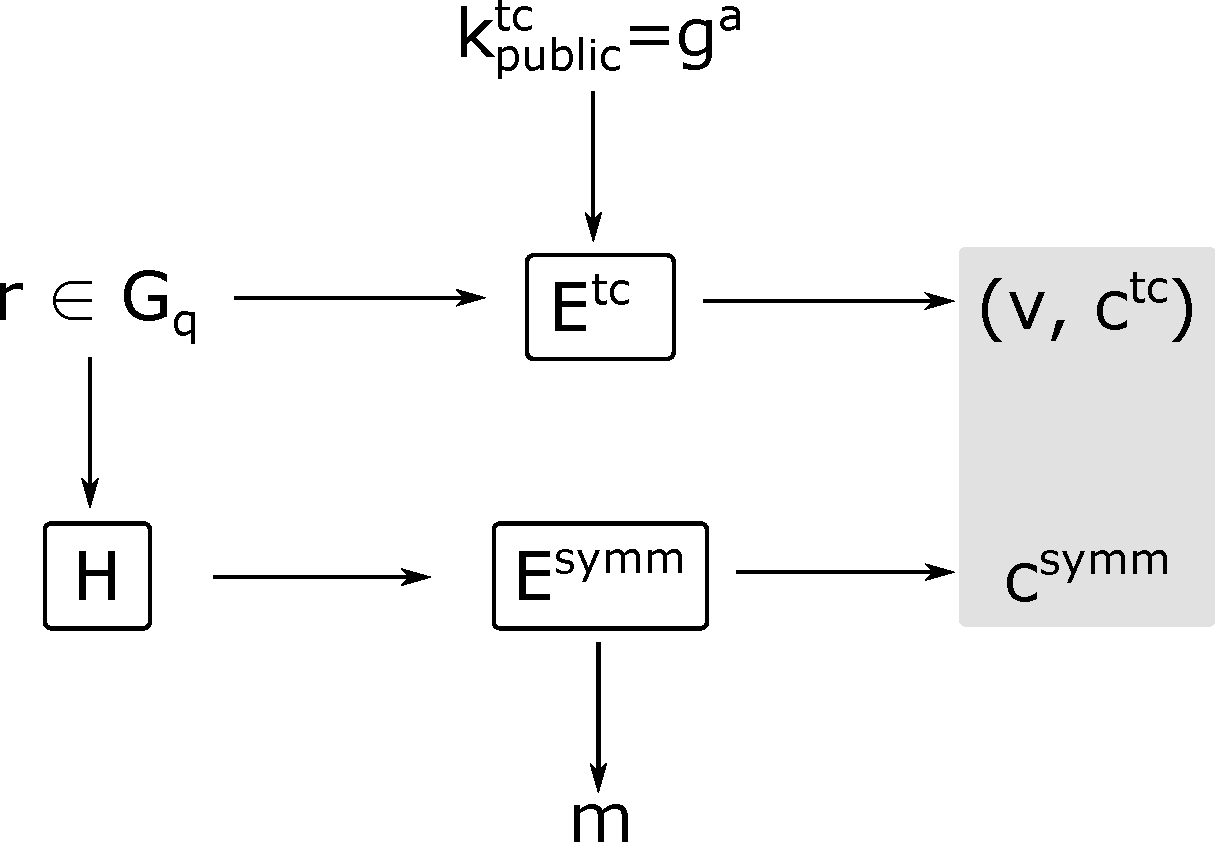
\includegraphics[width=0.4\textwidth]{dia/hybrid_scheme.pdf}
    \caption{Übersicht über das umgesetzte hybride Verschlüsselungsschema.}
    \label{fig:hybrid_scheme}
\end{figure}

\subsection{Service und Setup-Verfahren}

% Setup: Clients, KeyParameter, ThresholdParameter
% auf bereits in impl-pseudonymity geschriebenes zurückgreifen

Um die Parameter für das kryptographische Schwellwertschema setzen zu können, wurde die Konfigurationsoberfläche erweitert. Hier müssen nun Angaben zur Schlüsselstärke, zu beteiligten Teilnehmern und erforderlichen Anzahl an Teilnehmern für die Entschlüsselung eines Datenbankeintrages gemacht werden.

Anschließend können berechtigte Benutzer die Aufdeckung eines Pseudonyms über das Webinterface anfragen. Anschließend werden von den teilnehmenden Clients die partiellen Entschlüsselungen entgegengenommen. Liegen ausreichend partielle Verschlüsselungen vor, so werden diese mithilfe der Bibliothek kombiniert und damit der Halter des Pseudonyms entschlüsselt und aufgedeckt. 

\subsection{Client-Anwendung}

%- Shares empfangen und verschlüsselt abspeichern
%
%- Enthält Webserver um Shares niemals auf dem Server speichern zu müssen

Für Teilnehmer, die an dem Schwellwertschema beteiligt sind, wurde eine konsolenbasierte Anwendung entwickelt, die die folgende Funktionalität bereitstellt:

Clients melden sich zu Beginn an dem Pseudonym-Service an und können in der anschließenden Setup-Phase mit in das Verfahren integriert werden. Jeder teilnehmende Client empfängt nach der Generierung das für ihn bestimmte Share vom Server und speichert dieses verschlüsselt lokal ab. Hierzu enthält die Anwendung einen lokalen Webserver. Dies ermöglicht es dem Pseudonym-Service die \textit{Shares} nicht speichern und nach der Generierung sofort entfernen zu können. 

Anschließend können sich Teilnehmer regelmäßig nach neuen Anfragen zur Aufdeckung eines Pseudonyms erkundigen. Wurde eine neue Anfrage empfangen, so kann der Teilnehmen diese annehmen oder ablehnen. Die Annahme führt zur Berechnung einer partiellen Entschlüsselung mithilfe der Bibliotheksfunktion, die anschließend an den Pseudonym-Service gesendet wird.

\subsection{Proxy}

%- Empfängt PublicKey vom Service und nutzt ihn zur Nachrichtenverschlüsselung

Das im Syslog-Proxy implementierte Plugin zur Pseudonymisierung empfängt während der Initialisierung den während der Schlüsselerzeugung generierten öffentlichen Schlüssel vom Pseudonym-Service. Bei einer eintreffenden Syslog-Nachricht werden die zu pseudonymisierenden Daten mit diesem Schlüssel unter Nutzung der Bibliotheksfunktion verschlüsselt und zusammen mit den bereits in Abschnitt \ref{sec_impl_pseudonymity} beschriebenen weiteren Daten an den Service gesendet.

\section{Evaluation}

\label{sec_impl_evaluation}

Inklusive Problemen, ...
















\chapter{Ergänzende und alternative Datenschutztechniken}

\label{cha_alternatives}

%\begin{itemize}
%  \item \textbf{Alternativen} Welche alternativen oder ergänzenden Vorgehensweisen zu Pseudonymisierung + kryptographisches Schwellwertschema gibt es und welche Eigenschaften, Vor- und Nachteile besitzen sie?
%  \item \textbf{Umsetzung} Wie könnten diese Alternativen im Prototypen umgesetzt werden?
%\end{itemize}

% Generalisierung (zb nur noch Abteilung betrachten)
% Löschung
% Rauschen hinzufügen zB Zeitstempel plus normalverteilten Zufallswert (Christian)
% ...
%

% Siehe auch 
% Niksefat et. al.: Privacy issues in intrusion detection systems: A taxonomy, survey and future directions
%
%- Hash functions
%- Bloom filters
%- Homomorphic encryption
%- Secure multiparty computation
%- Z-String
%- Concept hierarchy
%- Differential privacy
%- Other classical techniques: Removal, Perturbation (Adding noise), Shifting (for example all timestamps to preserve interval lengths but hide real datetime)



Der in dieser Arbeit verfolgte Ansatz der Pseudonymisierung unter Einsatz kryptographischer Schwellwertschemata ist nicht für alle Arten von Logdaten sinnvoll. Sollen beispielsweise Zeitstempel verändert werden, um keine direkten Rückschlüsse auf eine Person durch Kombination mit typischen Verhaltensmustern zu ermöglichen, auf der anderen Seite jedoch zumindest grobe Erkenntnisse aus dem Zeitstempel für die Anomalieerkennung genutzt werden, so kann eine auf Pseudonymisierung basierende Lösung dies nicht leisten. 

Daher werden in diesem Abschnitt ergänzende Techniken zum Erhalt der Privatspäre eines Arbeitnehmers bei der Speicherung von Logdaten dargestellt und erläutert, wie diese in den entwickelten Prototyp eingebunden werden können. Natürlich können auch mehrere kombinierte Techniken für einzelne Logdaten, die aus mehreren Feldern bestehen, sinnvoll sein. Mit Zeitstempeln versehene Logdaten eines Türschließsystems, die die Benutzerkennungen der Mitarbeiter enthalten, könnten so beispielsweise durch Pseudonymisierung der Benutzerkennungen und Verrauschung der Zeitstempel geschützt werden.

Eine Übersicht über weitere in sehr speziellen Einsatzgebieten zu nutzende Datenschutztechniken wie Bloomfilter oder der Einsatz homomorpher Verschlüsselung sind in \cite{niksefat2017privacy} zu finden.

\section{Unterdrückung} % Suppression

Als ergänzende Maßnahme für Datenfelder, die für die Anomalieerkennung nicht benötigt werden, aber Rückschlüsse auf den Benutzer zulassen, kommt die Unterdrückung in Frage. Hierbei wird der Wert des Feldes schlicht entfernt oder durch eine Konstante ersetzt. 

Ein Beispiel im Kontext dieser Arbeit ist die Unterdrückung von IP-Adressen eines durch einen Arbeitnehmer benutzten Rechners für Logdaten, in denen auch der Benutzername enthalten ist. Beim Einsatz von Pseudonymisierung könnte die Zuordnung von Benutzer zu Pseudonym erleichtert werden, wenn der Arbeitnehmer dem physischen Gerät zu einem Zeitpunkt zugeordnet werden kann und die IP-Adresse des Geräts noch in den Logdaten enthalten ist.

\section{Generalisierung}

Bei der Generalisierung wird der Feldinhalt durch einen Wert ersetzt, der das gleiche Konzept beschreibt, jedoch allgemeiner ist. Durch mehrfache Verallgemeinerung entstehen sogenannte Generalisierungshierarchien \todo{Beispiel, Diagramm?}, wobei die Stufe der höchsten Generalisierung hier gleichbedeutend mit der Unterdrückung ist, da jeder Wert durch den konstanten Wert der höchsten Generalisierungsstufe ersetzt wird.

Ein Beispiel im Unternehmenskontext dieser Arbeit ist die Generalisierung eines Mitarbeiters zu seiner Arbeitsgruppe oder Abteilung -- eine Information, die für die Anomalieerkennung ausreichend sein könnte, wenn es beispielsweise um Zugriffe auf Ressourcen geht, die für bestimmte Abteilungen üblich, für andere jedoch ungewöhnlich sind. Dieses könnte zusätzlich zur Pseudonymisierung ausgeführt werden, um der Anomalieerkennung zusätzliche Daten zur Verfügung zu stellen, ohne die Identität eines Nutzers direkt offenzulegen.

\section{Verrauschen} % Hinzufügen von Rauschen

Diese Maßnahme verändert den Wert eines Datenfeldes, indem diesem Feld Werte aus einer Wahrscheinlichkeitsverteilung hinzugefügt werden (statistisches Rauschen). 
Hierdurch lassen sich die Rückschlüsse auf einen Nutzer aus einem einzelnen Datensatz verringern, aber die Gesamtverteilung bleibt erhalten bzw. lässt sich leicht berechnen. 
So können zumindest Abweichungen von Durchschnittswerten zur Anomalieerkennung genutzt werden. 
Es wird jedoch eine ausreichend große Datenmenge benötigt. Alternativ lassen sich zumindest Aussagen über den Bereich treffen, in dem ein Wert sich befinden muss. Dies könnte beispielsweise beim Verrauschen von Ereigniszeitstempeln sinnvoll sein, bei dem zwar nicht auf den konkreten Zeitpunkt geschlossen werden kann, aber zumindest Aussagen darüber getroffen werden können, ob das Ereignis in einem üblichen Intervall, wie in den normalen Bürostunden, auftrat.

Die Maßnahme ist jedoch nur für bestimmte Felder bzw. Datenarten sinnvoll einsatzbar. Gegenbeispiele sind unter anderem Freitextfelder, wie Benutzernamen, oder Felder für Aufzählungstypen, wie Raumnummern, die sich mit Rauschen nicht sinnvoll verändern lassen. 

\section{Nutzung von Hashverfahren}

Neben der zufälligen Generierung von Pseudonymen, wie es in dieser Arbeit genutzt wird, ist auch die Nutzung von Hashwerten als Pseudonym für Daten denkbar. Dies würde die Verknüpfbarkeit von Logdaten ermöglichen, da für gleiche Daten der gleiche Hashwert berechnet wird. Durch den geschickten Einsatz von zusätzlichen zeitabhängig wechselnden Eingaben für das Hashverfahren (sogenannte \textit{Salts}) ließe sich auch die nötige Verknüpfbarkeit für die Anomalieerkennung gegenüber dem Schutz der Privatsphäre eines Benutzers abstimmen.\\
Auf der anderen Seite wäre der Einsatz von Hashverfahren bei einem kleinen Wertebereich für Eingaben wie Benutzernamen anfällig für Wörterbuchangriffe (vgl. Abschnitt \ref{sec_state_se}). Außerdem wären auch Rückschlüsse auf den Pseudonymhalter nicht ohne zusätzlichen Aufwand möglich.

Für Datenfelder, bei denen nur die Verknüpfbarkeit, jedoch nicht der ursprüngliche Wert, für die Anomalieerkennung entscheidend ist und deren Wertebereich ausreichend groß ist, können Hashverfahren sinnvoll sein. \todo{Beispiel}

\section{Vorgehen zur Integration}

Die Integration der vorgestellten Datenschutztechniken in den entwickelten Prototyp stellt kein Problem dar. Die jeweiligen Techniken können, wie in Abschnitt \ref{sec_integration_in_ossim_plugins} beschrieben, als Plugins entwickelt werden. Hierbei entsteht je nach Datenschutztechnik unterschiedlicher Aufwand.

Für die Generalisierung und das Verrauschen müssen beispielsweise eingabedatenabhängige Plugins entstehen. Die Generalisierung von Zeitstempeln (Generalisierung auf Minute, Stunde, ... oder selbst gewählte Zeitabschnitte) unterscheidet sich beispielsweise stark von der Generalisierung der Umgebung eines Mitarbeiters (unternehmensspezifische Generalisierung auf Arbeitsgruppe, Abteilung, ...). Die Unterdrückung oder Nutzung von Hashverfahren kann hingegen unabhängig von den Eingaben entwickelt werden.

Für Datenquellen können diese Plugins nun einzeln oder in Kombination, wie in Abschnitt \ref{sec_integration_in_ossim_datasource_config} beschrieben, genutzt werden. Durch diesen Ansatz lässt sich für jede Datenquelle abhängig von verwendeten Anomalieerkennungsverfahren eine gute Abwägung zwischen Nutzbarkeit der Daten und Schutz der Privatsphäre eines Arbeitnehmers schaffen.

\chapter{Fazit}

\label{cha_final}

%You generally cover three things in the Conclusions section, and each of these usually merits a separate subsection:
%1. Conclusions
%2. Summary of Contributions
%3. Future Research

%Conclusions are not a rambling summary of the thesis: they are short, concise statements of the inferences that you have made because of your work. It helps to organize these as short numbered paragraphs, ordered from most to least important. All conclusions should be directly related to the research question stated in Section 4. Examples:
  %1. The problem stated in Section 4 has been solved: as shown in Sections ? to ??, an algorithm capable of handling large-scale Zylon problems in reasonable time has been developed.
  %2. The principal mechanism needed in the improved Zylon algorithm is the Grooty mechanism.
  %3. Etc.

%The Summary of Contributions will be much sought and carefully read by the examiners. Here you list the contributions of new knowledge that your thesis makes. Of course, the thesis itself must substantiate any claims made here. There is often some overlap with the Conclusions, but that's okay. Concise numbered paragraphs are again best. Organize from most to least important. Examples:
  %1. Developed a much quicker algorithm for large-scale Zylon problems.
  %2. Demonstrated the first use of the Grooty mechanism for Zylon calculations.
  %3. Etc.

%The Future Research subsection is included so that researchers picking up this work in future have the benefit of the ideas that you generated while you were working on the project. Again, concise numbered paragraphs are usually best. 



%- Ansatz: gut geeignet den Zielkonflikt zu lösen
%- System erfüllt die Anforderungen 
%- Parameteranpassbarkeit macht den Einsatz von Anomalieerkennungssystemen möglich
%- Abwägung zwischen Anom. und Privatsphäre -> Parameterwahl offen und kontextabhängig
%- Evaluation: für produktiveinsatz wohl noch arbeit notwendig



In dieser Arbeit wurde das Zusammenspiel von Pseudonymisierung und kryptographischen Schwellwertschemata als Lösung für die datenschutzgerechte Speicherung von Logdaten untersucht. 
%Pseudonymisierung
Als zentrale Anforderung an die Pseudonymisierung wurde die für unterschiedliche Einsatzkontexte per Parameter anpassbare Pseudonymwechselstrategie ausgemacht. Generell einsetzbare Parameter stellen die Nutzungshäufigkeit und das Zeitintervall der maximalen Nutzungsdauer dar. 
%Schwellwertschema
Es wurde das Feld der kryptographischen Schwellwertschemata untersucht und ein Schema auf Basis von Shamirs Secret Sharing und dem ElGamal-Verfahren ausgewählt sowie Verbesserungen in Form von \textit{Elliptic Curve Cryptography}, dezentraler Schlüsselgenerierung und komplexen Zugriffsstrukturen dargestellt.
%Identifikation
Das Problem der Identifikation bestehender Pseudonyme für verschlüsselte Daten wurde als zentrales Problem bei der Kombination beider Verfahren ausgemacht und verschiedene Lösungsansätze diskutiert. Ein Ansatz basierend auf der Nutzung von MACs als einfache Form deterministischer Verschlüsselung stellte sich für das entwickelte System als am geeignetsten heraus.
%Eingriff
Zusätzlich wurden verschiedene Ansätze für den Eingriff in den Logdatenfluss zwischen Quelle und SIEM-System betrachtet und ein Proxy-basierter Ansatz als sinnvolle Balance von frühestmöglicher Pseudonymisierung und praktischer Einsetzbarkeit ausgemacht.
%Architektur für System
Aus den beschriebenen Verfahren wurde ein verteiltes System entworfen, das in den Logdatenfluss eingreift, um Logdaten zu pseudonymisieren. Anschließend gibt es berechtigten Benutzern im Fall des Verdachts auf einen Insider-Angriff die Möglichkeit, die Aufdeckung von Pseudonymen zu beantragen bzw. über einen solchen Antrag zu entscheiden.

% Umsetzung
% Threshold Bib, die in anderern Anwendungen eingesetzt werden kann
Basierend auf diesen theoretischen Betrachtungen wurde ein Prototyp des entworfenen Systems implementiert, der Logdaten über das Syslog-Protokoll entgegennimmt. Neben der Entwicklung der verschiedenen Komponenten des verteilten Systems erwies sich inbesondere die Entwicklung des kryptographischen Schwellwertschemas als zentrale Herausforderung. Entgegen den Erwartungen vor Erstellung der Arbeit scheint es keine quelloffene und überprüfte Bibliothek zu geben, die die benötigten Funktionen bereitstellt -- eine Lücke, die die in dieser Arbeit entwickelte Bibliothek füllen kann. Dies erfordert jedoch eine ausgiebige Überprüfung durch erfahrene Kryptographen.

% Ergänzende Ansätze in Kapitel 6
In einem weiteren Kapitel wurden ergänzende Datenschutztechniken zu dem verfolgten Ansatz dargestellt, da die Pseudonymisierung nicht für alle Arten von Daten sinnvoll einsatzbar ist. Zusätzlich wurde ihre Einbindung in den entwickelten Prototypen dargestellt.

% Löst die Arbeit den beschriebenen Zielkonflikt?
% Evaluation -> für produktiven Einsatz wohl noch Arbeit notwendig
Der in dieser Arbeit gewählte Ansatz zur datenschutzfreundlichen Speicherung von Logdaten ist gut geeignet, um (eingeschränkte) Verknüpfbarkeit dieser Daten zur Anomalieerkennung und durch das Mehraugenprinzip geschützte Aufdeckbarkeit eines möglichen Innentäters im Verdachtsfall zu ermöglichen. Im Gegensatz zu bisherigen Lösungen, die oftmals eine vertrauensvolle Partei für die Generierung und Aufdeckung von Pseudonymen voraussetzen, kann durch diesen Ansatz verteiltes Vertrauen mathematisch-technisch modelliert werden. Durch die parameterabhängige Erstellung von Pseudonymen kann 
abhängig von unterschiedlichen Anforderungen des Einsatzkontexts gut zwischen den Anforderungen der Anomalieerkennung und dem Recht auf informationelle Selbstbestimmung des Arbeitnehmers abgewogen werden. Ob dies auch den rechtlichen Anforderungen des BDSG genügt, bleibt allerdings noch zu beurteilen.

Der entwickelte Prototyp zeigt auch die praktische Einsetzbarkeit des Verfahrens. Wie in dem Evaluationsabschnitt bereits beschrieben, sind vor dem Produktiveinsatz des Systems gerade im Hinblick auf die Performanz noch einige Optimierungen vorzunehmen.

Insgesamt kann der Ansatz dieser Arbeit die Speicherung der zur Anomalie-basierten Erkennung von Insider-Angriffen erforderlichen Überwachungsdaten und die Privatsphäre eines Arbeitnehmers zusammenbringen. Verfahren der Anomalieerkennung können relativ unabhängig von dieser Datenspeicherung entwickelt werden. Lediglich die Wahl der Parameter für die Pseudonymisierung und damit die Verknüpfbarkeit verschiedener Logdaten muss für einzelne Verfahren getroffen werden. Damit ist ein Schritt zur datenschutzgerechten Erkennung und Verhinderung von Insider-Angriffen getan, auf dem kommende Arbeiten aufbauen können.

%\section{Contributions}
%
%- Zusammenarbeit von Pseudonymisierung + Schwellwertschema
%- Beleuchtung verschiedener Ansätze für das Suchproblem (Anwendung von Searchable Encryption für ...)
%- Prototypische Implementation
%- Implementation Schwellwertschema 

%\section{Future work}
%
%- Implementation:
%  - Verteilte Schlüsselgenerierung
%  - Performance (Elliptic Curve Crypto), ...
%  - Cryptographic Review
%  - Access structures (irgendwo noch erwähnen!! State Threshold?)
%- Parameterwahl für situationsabhängige Pseudonymisierung? (Evtl. dieses Problem in state noch ergänzen...) -> Forschungsarbeit notwendig
%- Auswirkungen für verteilte Systeme (Schlüssel, SearchableEncryption, ...)

Hierfür bietet das Themenfeld ausgehend von dem erreichten Stand dieser Arbeit noch einiges Potential für aufbauende Entwicklungs- und Forschungsarbeit. Der entwickelte Prototyp lässt sich noch an einigen Stellen optimieren:

\begin{itemize}
  \item Implementierung der verteilten Schlüsselgenerierung (siehe Abschnitt \ref{sec_state_threshold_distributed})
  \item Überprüfung der entwickelten Bibliothek für die Nutzung kryptographischer Schwellwertschemata durch erfahrene Kryptographen
  \item Performanzsteigerung durch die Nutzung von elliptischen Kurven (siehe Abschnitt \ref{sec_state_threshold_ecc})
  \item Ermöglichung von komplexen Zugriffsstrukturen, die über die 1:1-Zuweisung von Shares an Beteiligte hinausgehen (siehe Abschnitt \ref{sec_state_threshold_access_structures})
\end{itemize}

Neben diesen Implementierungsarbeiten bieten sich jedoch auch einige Fragestellungen für weiterführende Forschungen an:

\begin{itemize}
  \item Welche Auswirkungen hat die Wahl der Parameter für Nutzungshäufigkeit und zeitliche Begrenzung der verwendeten Pseudonyme für bestehende oder zu entwickelnde Anomalieerkennungsverfahren? Wie lässt sich also am besten zwischen dem Schutz der Privatsphäre eines Arbeitnehmers und erfolgreicher Anomalieerkennung vermitteln?
  \item Gibt es weitere (eventuell kontextabhängige) Parameter, die für die Pseudonymisierung genutzt werden sollten?
  \item Wie könnte ein System umgesetzt werden, das verteilte Datenverarbeitung -- also beispielsweise auch die Pseudonymisierung direkt in der Datenquelle -- ermöglicht? Insbesondere das Suchproblem nach bereits verwendeten Pseudonymen aus Abschnitt \ref{sec_state_se} muss hier betrachtet werden.
  %\item Gleiche Pseudonyme für unterschiedliche Daten eines Benutzers
\end{itemize}






% ================================Literature==============================

\begin{raggedright}         % Schaltet Blocksatz ab, erzeugt ein stimmigeres
                            %  Schriftbild im Literaturverzeichnis.
  \printbibliography        % Falls Biblatex verwendet wird.
  \label{sec:literaturverzeichnis}
\end{raggedright}

\end{document}

